% Document
\documentclass{article}

% Packages
\usepackage[utf8]{inputenc}                                                             % input encoding
\usepackage[T1]{fontenc}                                                                % font encoding
\usepackage[ngerman]{babel}                                                             % for German
\usepackage[left=2cm, right=2cm, top=2.5cm,bottom=2.5cm]{geometry}                      % for page size
\usepackage{natbib}                                                                     % for bibliography
\usepackage{graphicx}                                                                   % for images
\usepackage[font=normal,labelfont=bf,textfont=rm,position=bottom,skip=10pt]{caption}    % for captions
\usepackage{amsmath}                                                                    % for formulas
\usepackage{float}                                                                      % for images at right position
\usepackage[autostyle=true,german=quotes]{csquotes}                                     % for proper quotes
\usepackage{siunitx}
\sisetup{per-mode=symbol}                                         

% for MATLAB-codes
\usepackage{comment}
\usepackage{bm}
\usepackage{subfigure}
\usepackage{hyperref}
\usepackage{pdfpages} %fuer einfuegen von PDFs (Aufgabenstellung)
% for block comments

\bibliographystyle{agsm}

\newcommand{\geodaten}[1]{\underline{#1}}     % Vektor als Matrix

% Document start
\begin{document}
\begin{minipage}[c][\textheight][t]{\textwidth}
	\centering
	\begin{minipage}[c]{2cm}%
		
\includegraphics[height=2cm]{bilder/logo_gi}%
	\end{minipage}
	\hfill
	\begin{minipage}[c]{8cm}
		\centering
		\vspace*{2mm}
		\LARGE Universität Stuttgart\\[3mm]
		\Large Geodätisches Institut
	\end{minipage}
	\hfill
	\begin{minipage}[c]{2cm}%
		
\includegraphics[height=2cm]{bilder/logo_uni-stuttgart.png}%
	\end{minipage}\\[5mm]
	\rule{\textwidth}{0.5pt}\\[10mm]
	
	%  \vspace*{2cm} % kein Bild: diese Zeile "einkommentieren" ...
	\vspace*{1cm} % ... und diese "auskommentieren ..."
	{\huge {\textbf{Projekt Weltraummüll}}}\\[10mm]
	\vspace*{1cm} % ... und diese "auskommentieren" ...
	
	%  \vspace*{4cm} % kein Bild: diese Zeile "einkommentieren" ...
	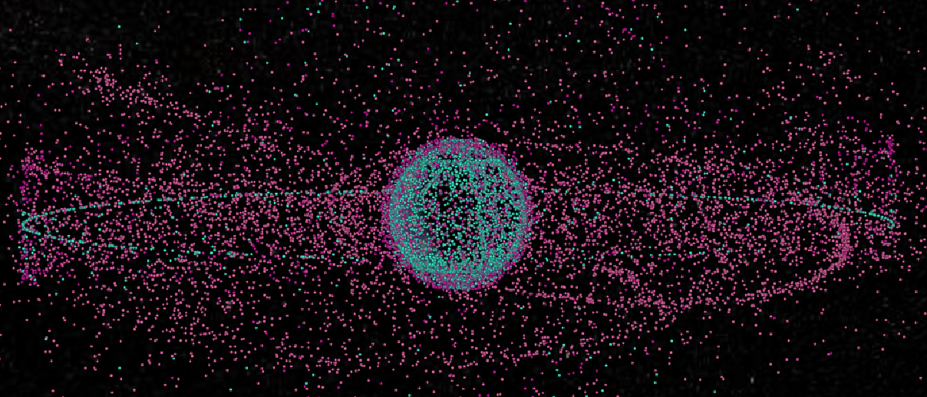
\includegraphics[height=6cm]{bilder/spacedebris.png}\\[10mm] % ... und diese "auskommentieren"
	\vfill
	Jiaxin Liu\\[2mm]
	Philipp Schollmeier\\[2mm]
	Torben Blei\\[2mm]
	Ziqing Yu\\[10mm]
	Stuttgart, 2022\\[5mm]
	\rule{\textwidth}{0.5pt}\\[5mm]
	\begin{minipage}{\textwidth}%
		\hfill
		\begin{minipage}[t]{0.1\textwidth}%
			\large\textbf{Betreuer:}%
		\end{minipage}
		\quad
		\begin{minipage}[t][3.0cm]{0.6\textwidth}%
			\large Prof. Dr.-Ing. Nico Sneeuw\\
			Universität Stuttgart\\[3mm]
		\end{minipage}
		\hfill
	\end{minipage}
\end{minipage}
\clearpage	

\section{Einleitung}
Die Zahl der Müllteile in der Erdumlaufbahn erfährt seit dem ersten künstlichen Satelliten Sputnik im Jahr 1957 ein starkes Wachstum. Bereits in den 70er Jahren warnte der amerikanische Astronom Donald Kessler vor den Gefahren dieser Entwicklung. Mit einer größeren Anzahl an Partikeln steige die Anzahl der Kollisionen zwischen Teilen. Jede solche Kollision führe zu neuen Wolken von Müllteilen und ab einer bestimmten Anzahl trete eine Kettenreaktion ein, in der ständig neue Kollisionen und neue Schrottteile entstünden. Dieses Szenario wird nach ihm Kessler-Syndrom genannt. Sollte es in einem bestimmten Orbit Realität werden, könnte dieser nicht mehr menschlich genutzt werden, was Beeinträchtigungen von Kommunikation, Navigation, Wetterbeobachtung usw. zur Folge hätte. \\
\begin{figure}[H]
	\centering
	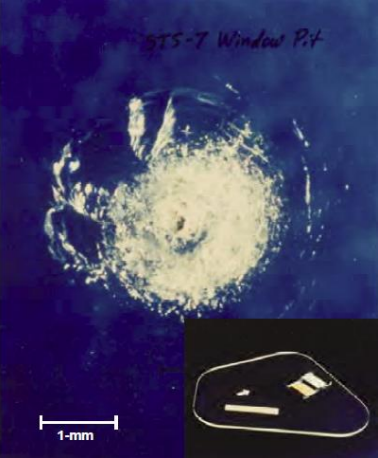
\includegraphics[width = 0.5\textwidth]{bilder/Debris.png}
	\caption{Beschädigung an einem Fenster der Challenger-Raumfähre nach Einschlag eines Raummüllteils, das Teil wurde auf eine Größe von 0,02 mm geschätzt \citep{carpenteruse}}
	\label{Debris}
\end{figure}
\noindent Im 21. Jahrhundert haben sich die Warnungen von Kessler zum Teil bestätigt. Am 10. Februar 2009 kollidierten die beiden stillgelegten LEO-Satelliten Iridium 33 und Kosmos 2251. Dabei entstanden über 100.000 Trümmerteile die seitdem in zwei Müllwolken um die Erde kreisen. Die International Raumstation genauso wie Satelliten müssen regelmäßig Ausweich-Manöver durchführen, um nicht von Raumschrott getroffen zu werden. Immer wieder kommt es auch zu Kollisionen mit kleineren Teilen, die von den Überwachungssystemen nicht verfolgt werden können. Was eine solche Kollision mit den meist mikroskopisch kleinen Teilen anrichten kann, zeigt \autoref{Debris}. \\\\
Vor allem in den letzten zwanzig Jahren hat sich durch das stärkere Aufkommen von kommerziell gestarteten Satelliten, das Wachstum der Partikelanzahl noch einmal erhöht. Die Gesamtzahl der Teile wird auf mehrere hundert Millionen geschätzt. Ein Teil dieser Partikel wird durch die Luftreibung ohne menschliches Eingreifen nach einer gewissen Zeit abstürzen. Diese passive Entsorgung wird in \autoref{sec:pass} untersucht. Der ständige Anstieg der Teile zeigt aber, dass dieser natürliche Vorgang nicht ausreichen wird, damit der Weltraum (insbesondere der stark genutzte Low Earth Orbit) auch in Zukunft für die Menschheit nutzbar bleibt. In den \autoref{sec:segel} und \ref{sec:sate} werden zwei verschiedene mechanische Ansätze zur aktiven Entfernung von Müllteilen diskutiert. Das vielleicht vielversprechendste weil ökonomisch beste Konzept ist das Laserbasierte. Dieses wird in \autoref{sec:laser} beleuchtet.	

\section{Raumobjekt Statistik}
Die TLE Daten aller bekannter Raumobjekten wurden von \href{https://www.space-track.org/auth/login}{Space-Track} angeboten. Die Objekten Klassifikation wurde per API von \href{https://discosweb.esoc.esa.int/}{DISCOSweb} von der ESA heruntergeladen. Die originalen TLE Daten sind in einigen Text-Dateien chaotisch geteilt, daher muss man zuerst die Daten organisieren und gleichzeitig die interessante Daten extrahieren. Dieser Schritt wurde mit Python gemacht und die Ergebnisse werden per Jahre per Objekt in csv Datei gespeichert. Danach liest man diese Datei in Matlab und generiert man die monatliche .mat Datein für die Analyse später.
\\\\
In \autoref{fig:objectcount} sind die Anzahl aller bekannten Raumobjekte von 1959 bis 2022. Obwohl in manche Jahren abstürzten mehr Objekten als die neu gesendete Körpern, sehen wir dass die Objektanzahl stieg überhaupt. Dieser positive Trend war besonders stark in letzten 2 Jahren, so dass man dieses Problem nicht mehre ignorieren kann. 
\begin{figure}[ht]\centering 
	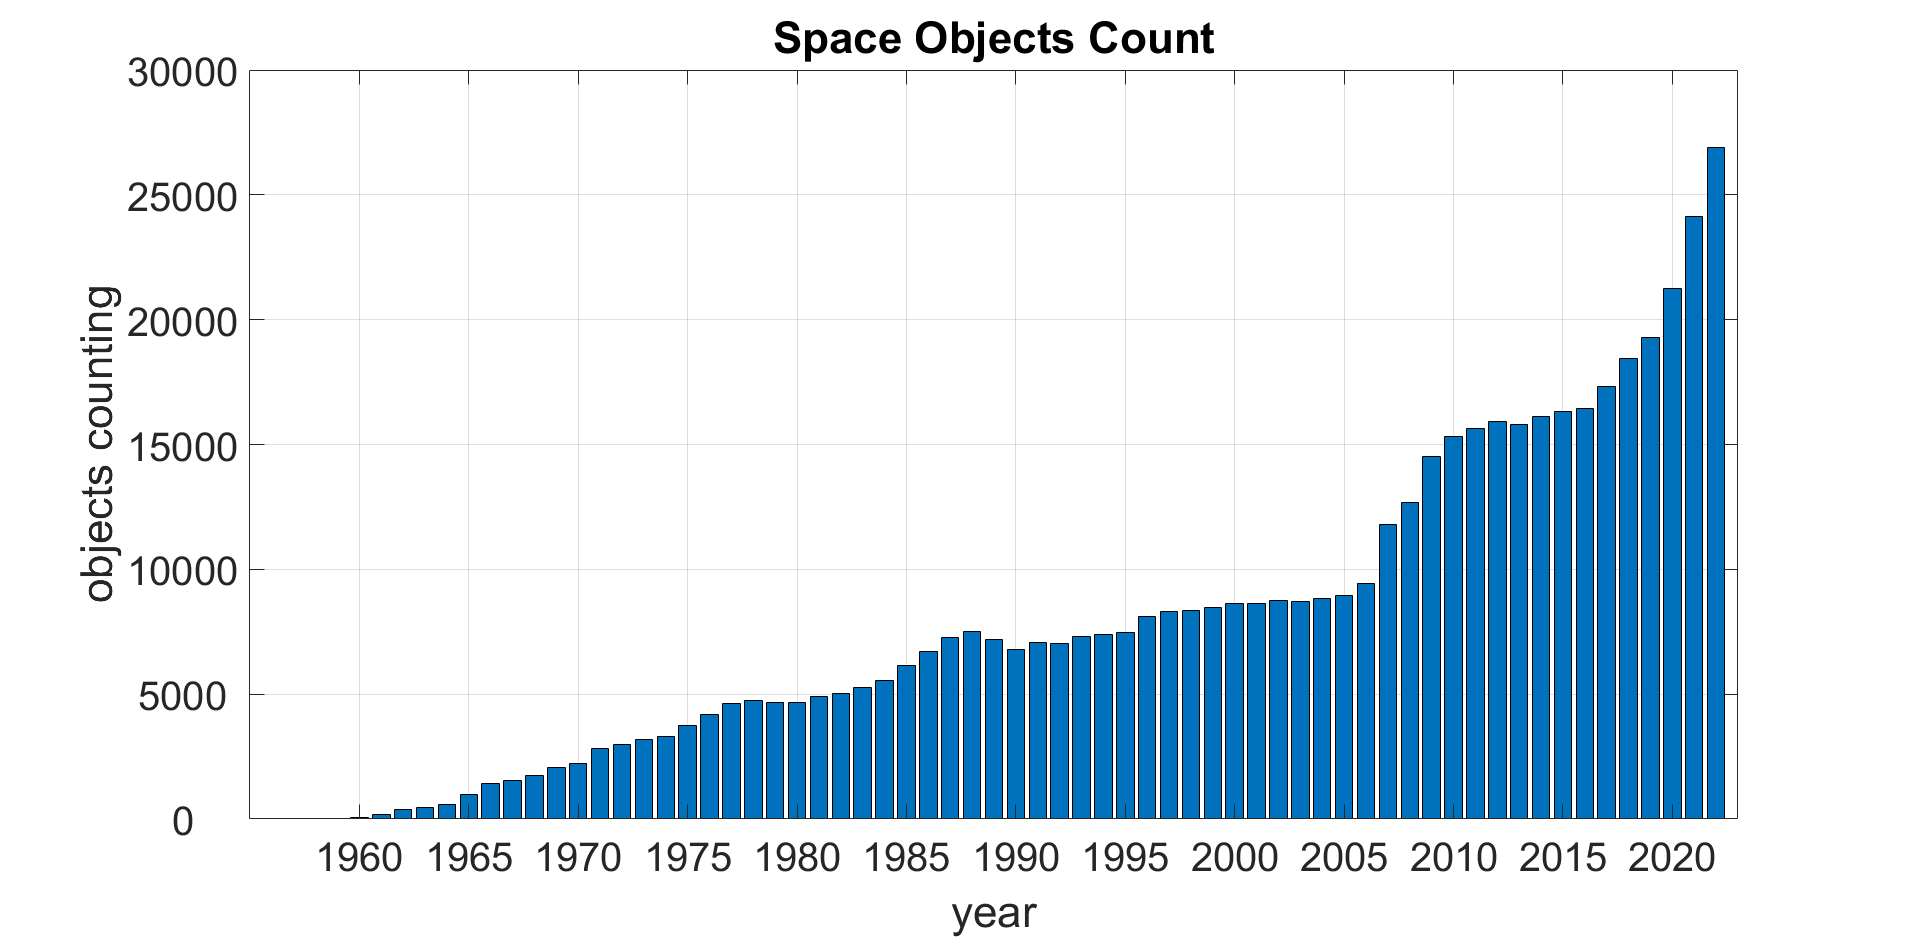
\includegraphics[width=0.9\textwidth]{images/all_obj_counts.png}
	\caption{Integration der Kreisbahnen von verschiedenen Höhen}
	\label{fig:objectcount}
\end{figure}
\\\\
In \autoref{fig:objectclassification} wird die die Objekt-Klassifikation im Jahr 2022 dargestellt. fast halbe bekannte Objekten sind 'Payload Fragmentation Debris' und 'Rocket Fragmentation Debris', die man nicht im Raum sehen will. Außerdem gibt es noch viele kleine Stücks, die für uns nicht 'sichtbar' sind. Je mehr Objekten im Raum existieren, desto höher ist die Möglichkeit, dass neue Dinge durch Kollision generiert könnte. Falls man dieses Problem nicht vorsichtig aufpassen, leisten wir selbe in Zukunft unvorstellbare Auswirkung.
\begin{figure}[ht]\centering 
	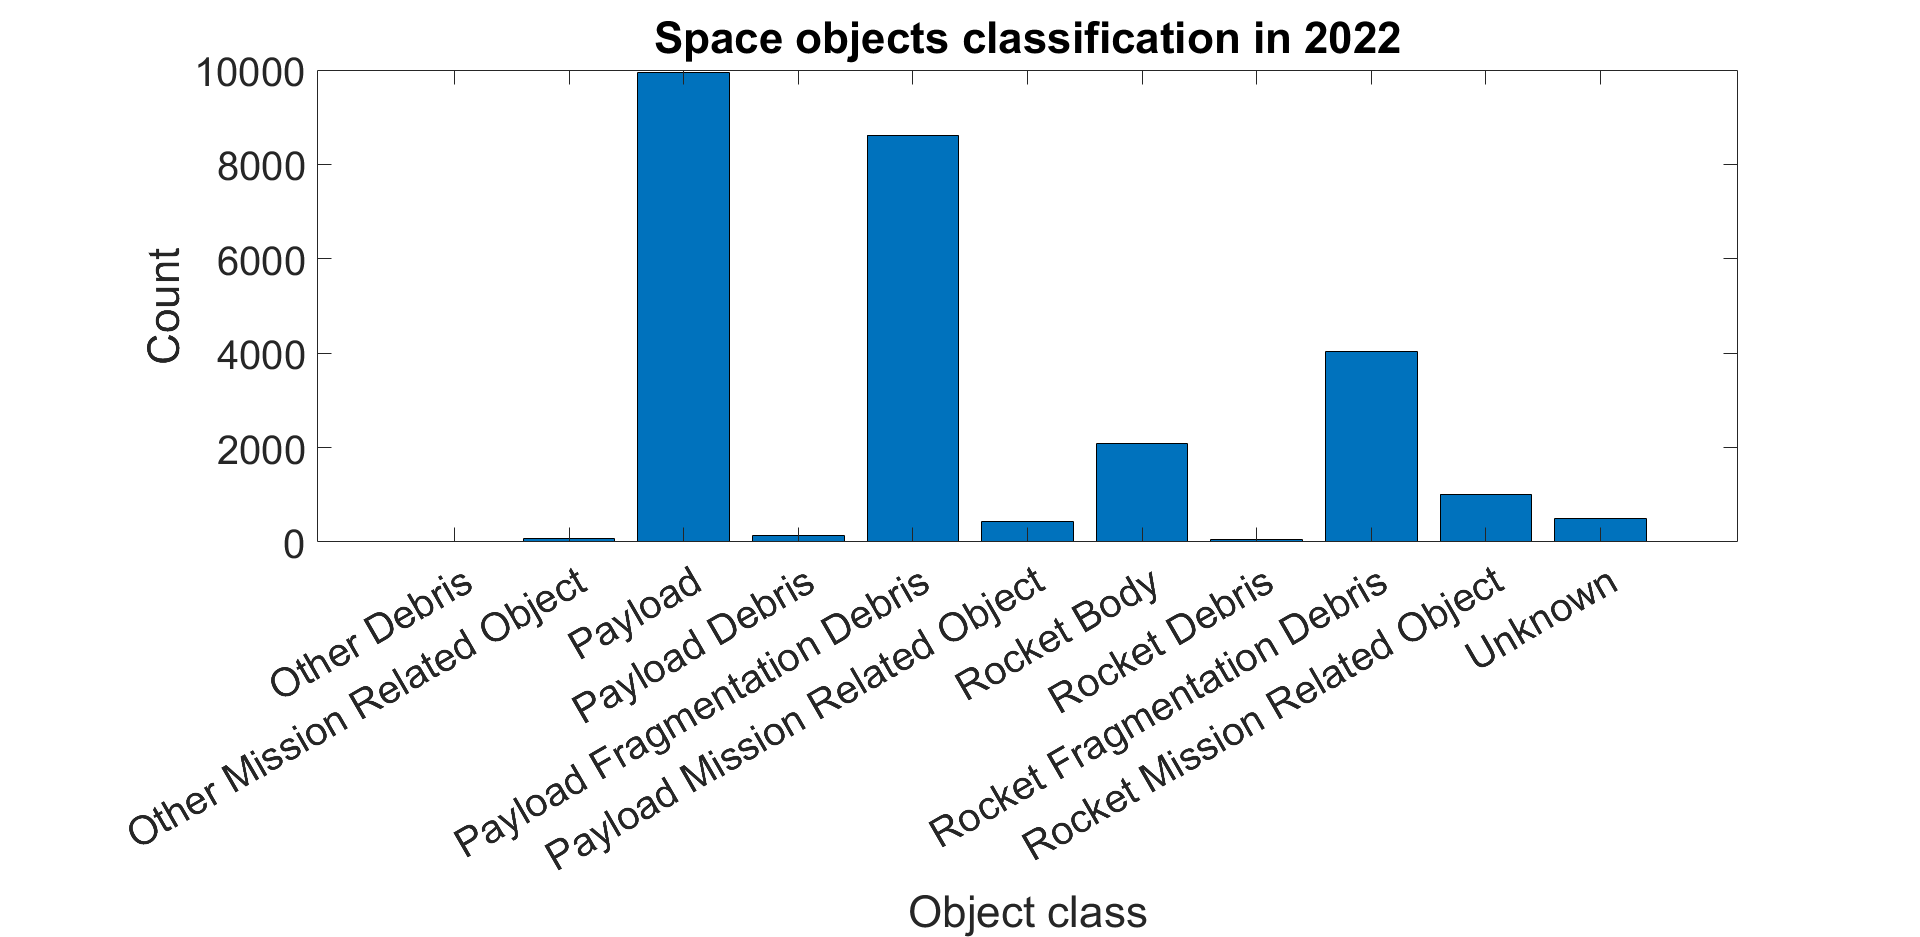
\includegraphics[width=0.9\textwidth]{images/obj_classification.png}
	\caption{Raumobjekten Klassifikation im Jahr 2022}
	\label{fig:objectclassification}
\end{figure}
\begin{figure}[htbp]
\centering
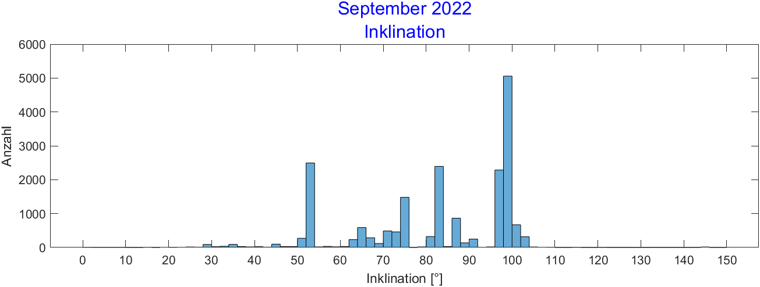
\includegraphics[width=1\textwidth]{bilder/Inklination.png}
\caption{Screenshot des in der Präsentation gezeigten GIF: die Inklination aller Objekte im LEO-Orbit von von 2005 bis 2022}
\label{Inklination}
\end{figure}\\\\
\noindent Die Inklination eines Satelliten ist eng mit seiner Nutzung verbunden. In \autoref{Inklination} ist leicht zu erkennen, dass die Inklination der meisten Objekte zwischen \SI{100}{\degree} und \SI{100}{\degree} liegt. Davon befinden sich Satelliten mit einer Inklination von etwa \SI{100}{\degree} wahrscheinlich in einer sonnensynchronen Umlaufbahn, während eine Inklination von \SI{63,4}{\degree} wird oft als kritische Inklination bezeichnet, weil sie keine Apogäumsdrift haben.
\clearpage
\begin{figure}[htbp]
\centering
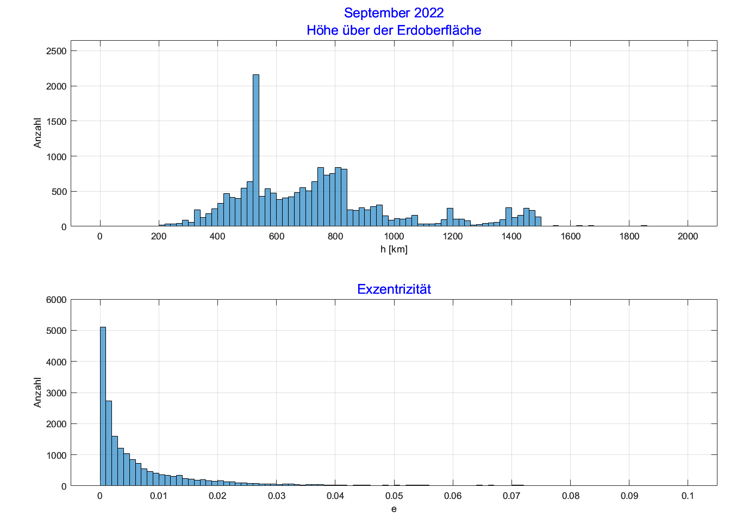
\includegraphics[width=1\textwidth]{bilder/Hoehe.png}
\caption{Screenshot des in der Präsentation gezeigten GIF: die Inklination aller Objekte im LEO-Orbit von von 2005 bis 2022}
\label{Hoehe}
\end{figure}
\noindent \autoref{Hoehe} zeigt die Verteilung der Exzentrizität und Höhe aller Objekte im LEO-Orbit. Fast alle Objekte sind zwischen \SI{200}{\kilo\meter} und \SI{1600}{\kilo\meter} konzentriert und haben eine sehr geringe Exzentrizität. Das bedeutet auch, dass dieses Gebiet mit extrem dichten Objekten mit Weltraummüll gefüllt ist, was einen erheblichen negativen Einfluss auf die Funktionsfähigkeit von Satelliten hat.
\clearpage
\begin{figure}[htbp]
\centering
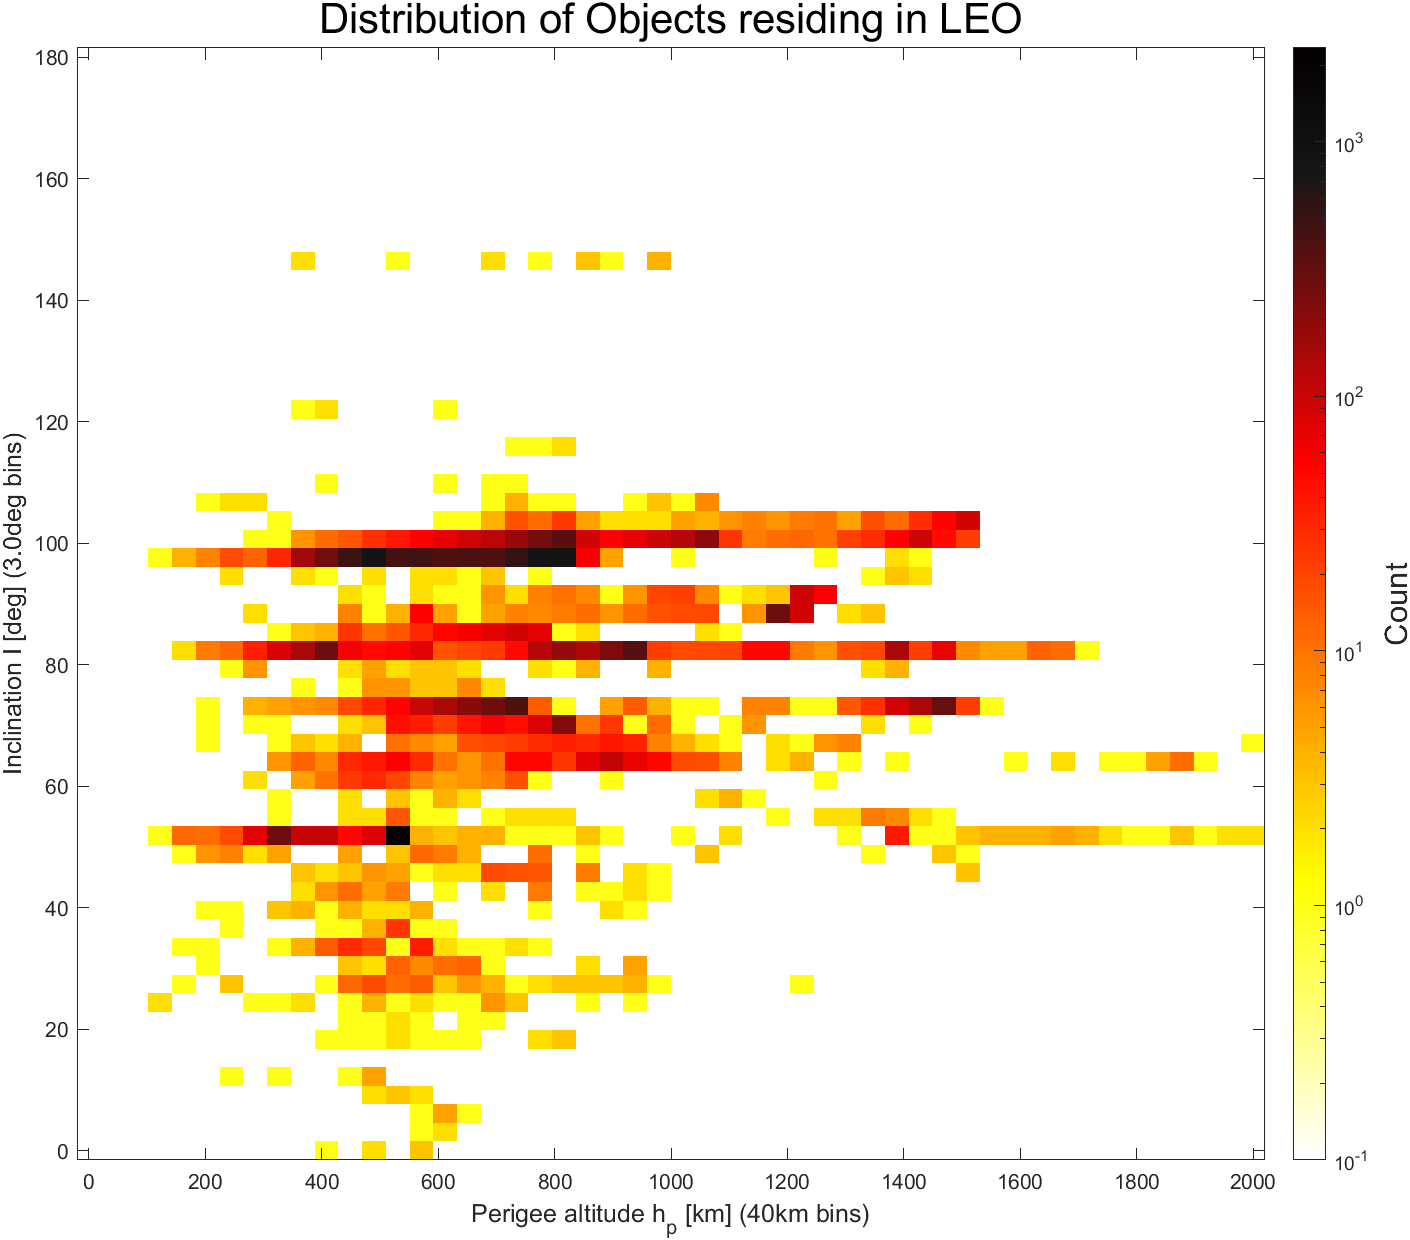
\includegraphics[width=0.5\textwidth]{bilder/Distribution_1.png}
\caption{Verteilung der Anzahl der Objekte im LEO als Funktion der Inklination und der Perigäumshöhe.}
\label{Distribution_1}
\end{figure}

\begin{figure}[htbp]
\centering
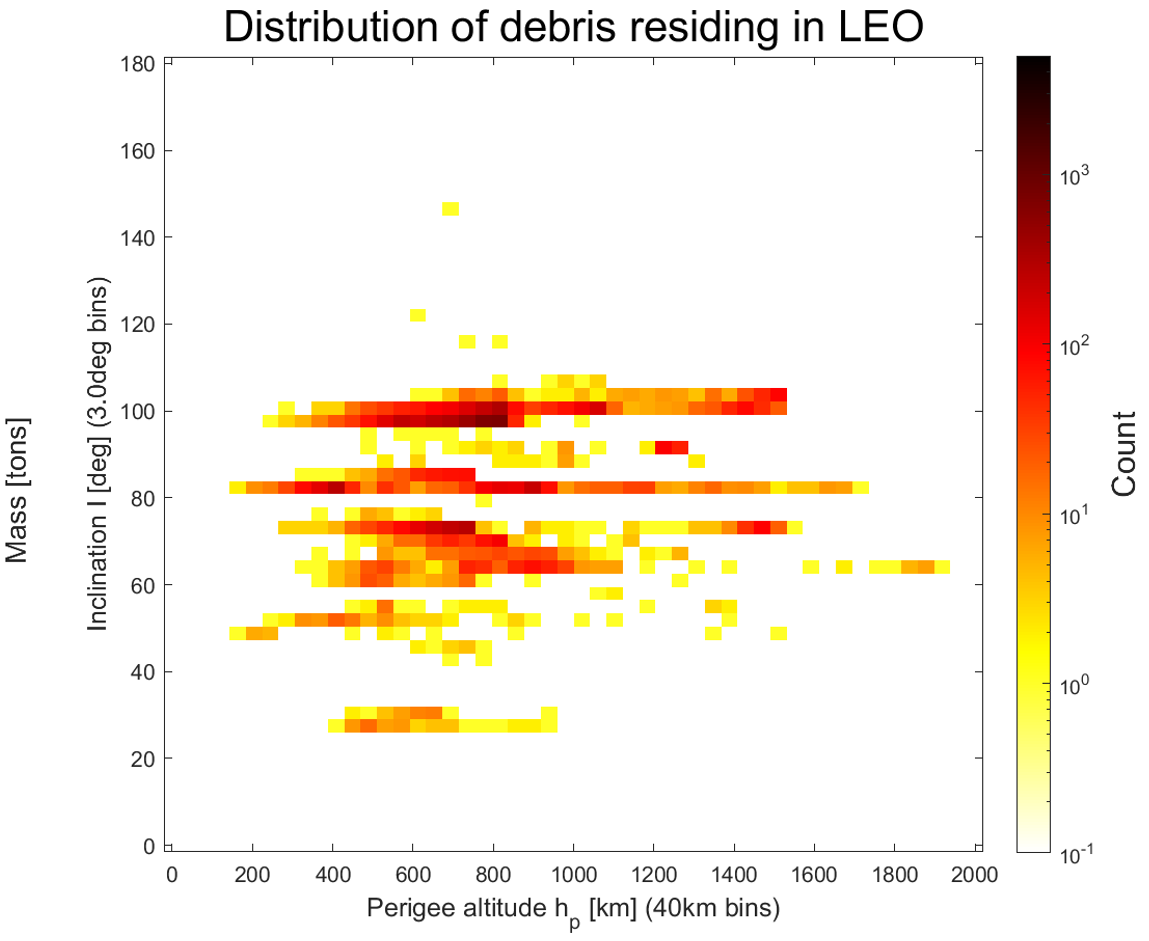
\includegraphics[width=0.5\textwidth]{bilder/Distribution_2.png}
\caption{Verteilung der Anzahl der space debris im LEO als Funktion der Inklination und der Perigäumshöhe.}
\label{Distribution_2}
\end{figure}
\noindent \autoref{Distribution_1} und \autoref{Distribution_2} zeigen die Verteilung aller Objekte und des Weltraumschrotts in der LEO-Orbit in einem zweidimensionalen Histogramm. Die Perigäumshöhe wird in \SI{40}{\kilo\meter}-Bins gezählt, während die Inklination in \SI{3}{\degree} - Bins gezählt wird. Der Vergleich zeigt, dass Gebiete mit einer hohen Dichte an Objekten auch eine große Menge an Weltraumschrott haben. Zum Beispiel gibt es mehrere tausend Objekte in einem Gebiet mit einer Höhe von 400-600 km und einer Inklination von etwa \SI{100}{\degree}. Gleichzeitig kann auch festgestellt werden, dass sich fast tausend Weltraumschrott im selben Gebiet versammelt haben, was sehr gefährlich ist.


\clearpage	
\section{Bahnintegration}\label{sec:pass}
Da dünne Luft in LEO Bereich existiert bremsen die Objekten sich langsam und sie werden am Ende auf die Erde fallen. Allerdings kommt dann die Frage: wie lang dauert dieser Prozess?
\\\\
\autoref{eq2} beschriebt die atmosphärische Widerstand des Objekts im Raum. $A$ ist die Querschnittfläche entlang Geschwindigkeitsrichtung, $m$ ist die Masse, wir nennen $A/m$ als ein Parametern, der 'Verhältnis von Fläche zu Masse' heißt. $\rho$ ist die Atmosphärendichte, $\bm{\dot{r}_a}$ und $\bm{\dot{r}}$ sind jeweils die Geschwindigkeit der Atmosphäre und Objekt. $C_d$ beschreibt die Form des Objekts im Raum, typische Werte sind bspw. 1 für Kugel und ca. 2.5 für ISS(Die Internationale Raumstation).
\begin{equation}\label{eq2}
	\frac{\bm{f}_{atm}}{m} = -\frac{1}{2} \cdot C_d \cdot \rho \cdot \frac{A}{m} \cdot \left(\bm{\dot{r}} - \bm{\dot{r}_a}\right) \cdot |\bm{\dot{r}} - \bm{\dot{r}_a}|
\end{equation}
Das bedeutet, bevor wir die Bahnintegration implementieren, müssen wir zunächst Raumobjekten bzw. Raumatmosphäre untersuchen.
\subsection{Atmosphärische Eigenschaft im Raum}
2 Atmosphäre Modelle sind untersucht nämlich Harris-Priester Modell \citep{harris1963relation} und MSIS-E-00 \citep{picone2002nrlmsise}. Bei Harris-Priester Model ist die Atmosphärische Dicht nur von Höhe abhängen und MSIS-E-00 ist ein viel präziseres Modell, bei dem geographische Ort, Höhe und auch Zeit eine Rolle spielen.
\\\\
Bei MSIS-E-00 Model ist die Atmosphärische Dichte von mehre Parametern abhängig, bspw. ellipsoidische Höhe, Länge, Breite und Zeit. In \autoref{fig:msise00_400km} sind die atmosphärische Dichte in der Höhe von \SI{400}{\kilo \meter} um 0:00 und 12:00 UTC. Man sieht eine offensichtliche Tag-Nacht Phänomen zwischen 2 Bildern. Es wird angenommen, dass die Atmosphärische Dichte in eine bestimmte Höhe in Länge Zeit relativ konstant bleiben.
\begin{figure}[ht]\centering 
	\subfigure[]{
		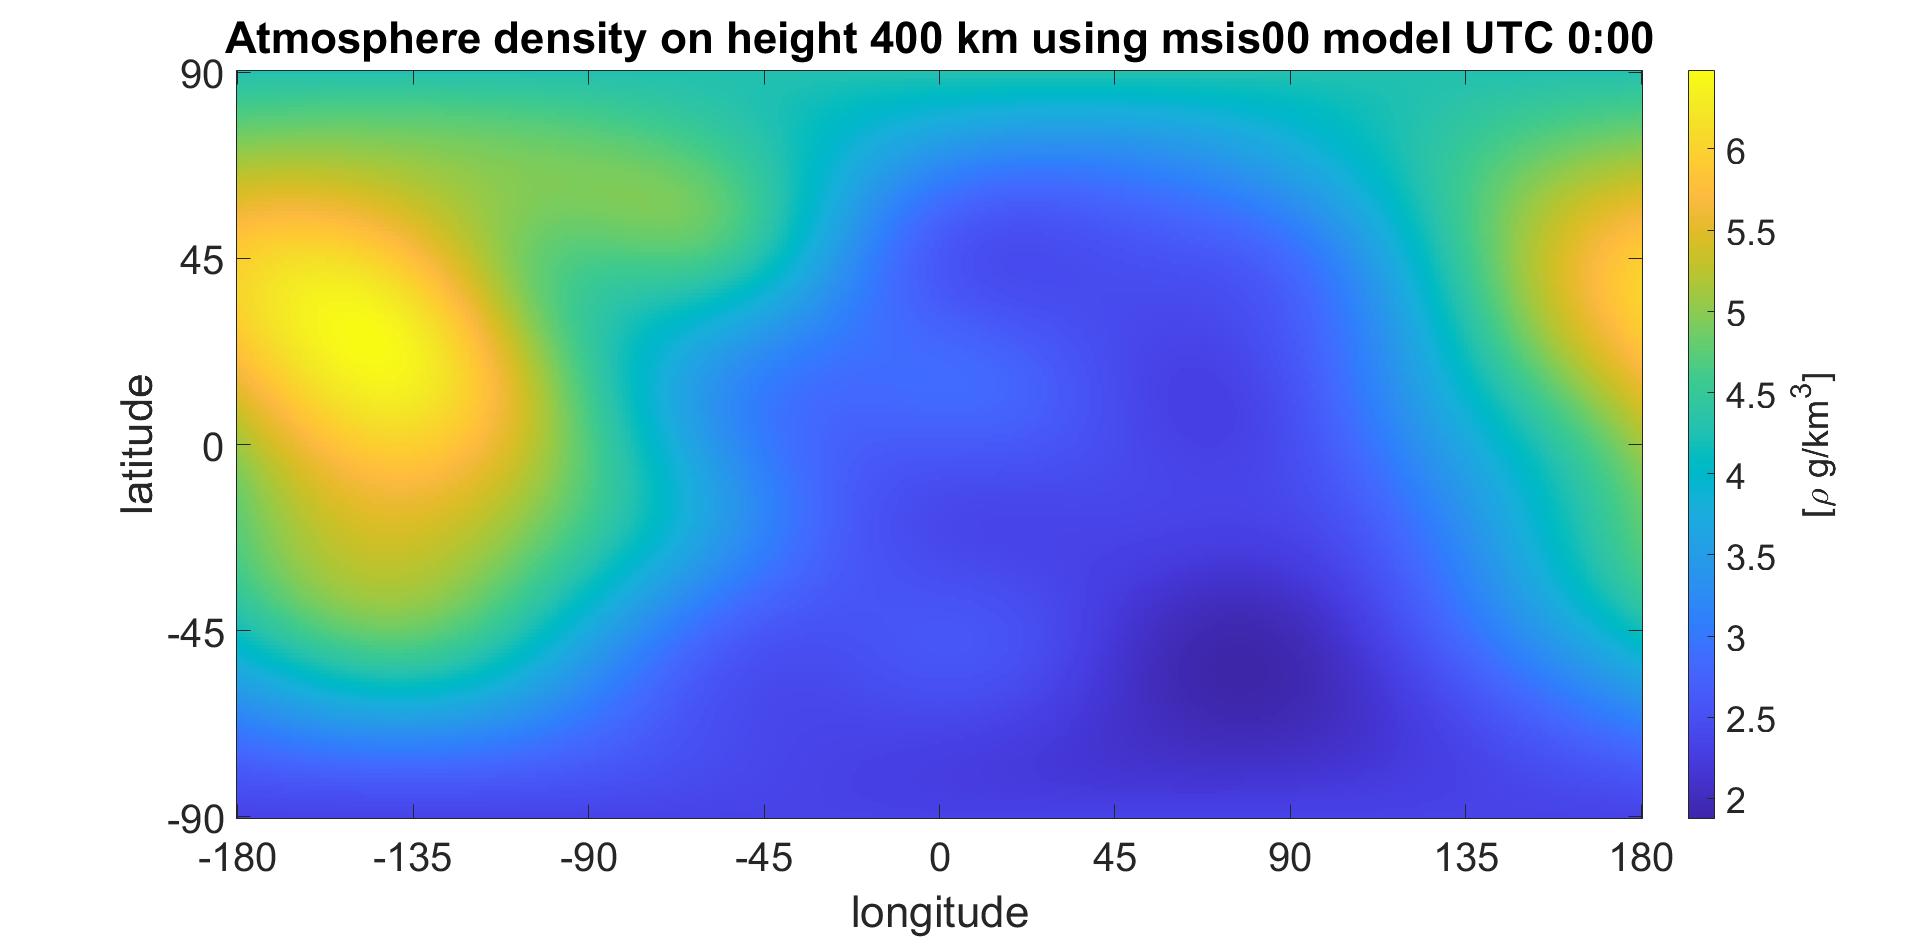
\includegraphics[width=0.9\textwidth]{images/msis_day.png}}
	\subfigure[]{
		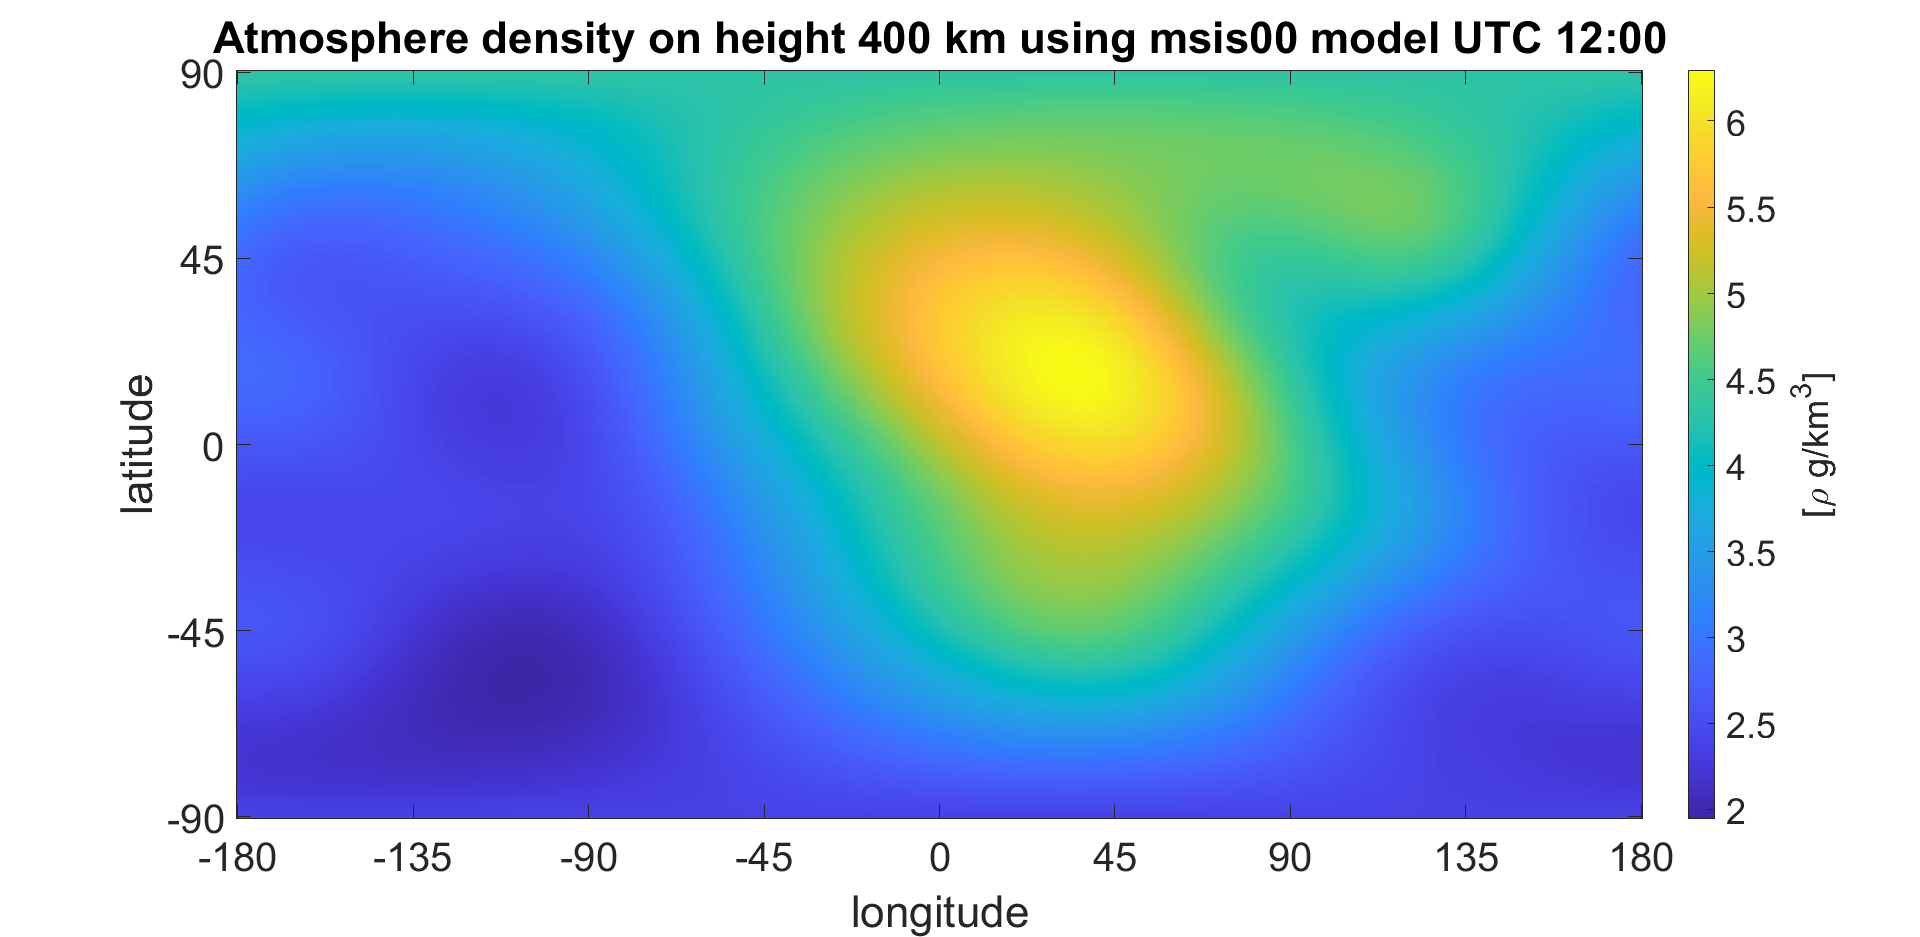
\includegraphics[width=0.9\textwidth]{images/msis_night.png}}
	\caption{Atmosphärische Dichte \SI{400}{\kilo \meter} über die Erde um 0:00 und 12:00 UTC}
	\label{fig:msise00_400km}
\end{figure}
\\
In \autoref{fig:compare_model} wird die Differenzen zwischen beiden Modellen dargestellt. Die Dichte von Harris-Priester Modell sind größer als die von MSIS-E-00 Modell sowohl über Nordpol als auch über Äquator. Außerdem sinkt die Differenz zwischen beiden Modellen mit steigende Höhe.
\\\\
In Praxis dauert die Bahnintegration ziemlich lang mit MSIS-E-00 Modell. Damit man die Zeit sparen und mehr Ergebnisse kriegen kann, verwendeten wir Harris-Priester Modell, obwohl MSIS-E-00 präziser ist.
\begin{figure}[ht]\centering 
	\subfigure[]{
		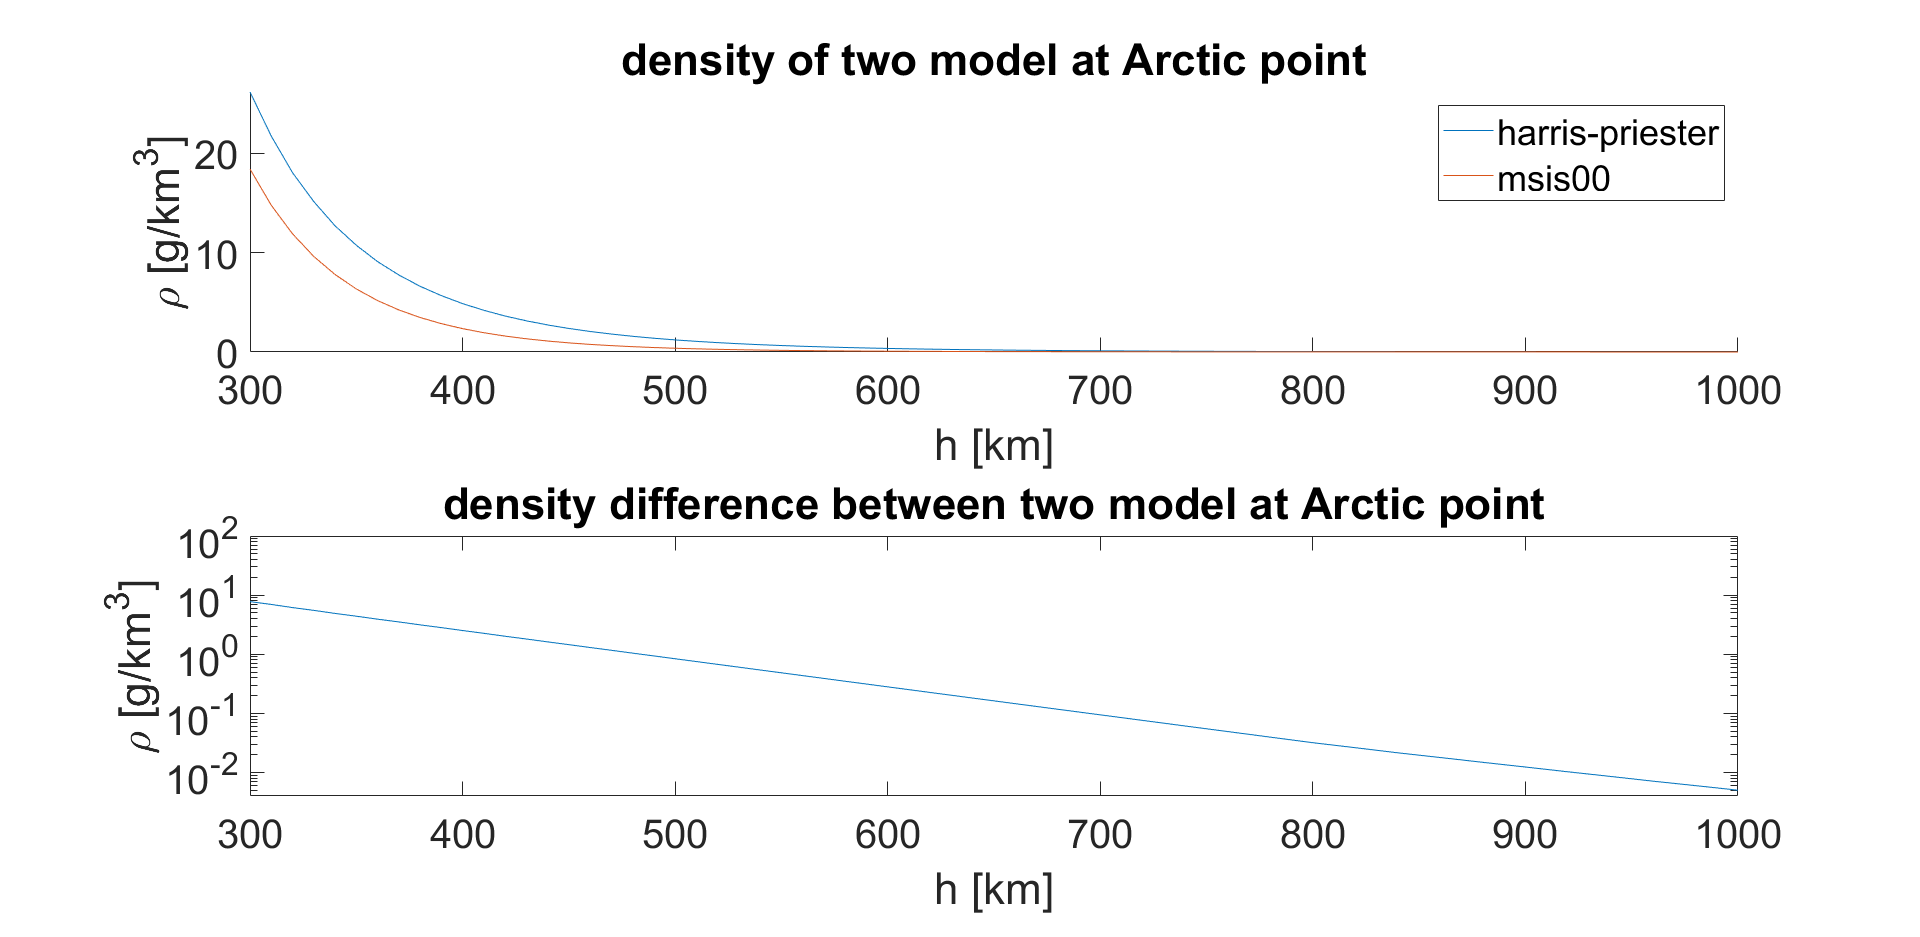
\includegraphics[width=0.9\textwidth]{images/compare_arctic.png}}
	\subfigure[]{
		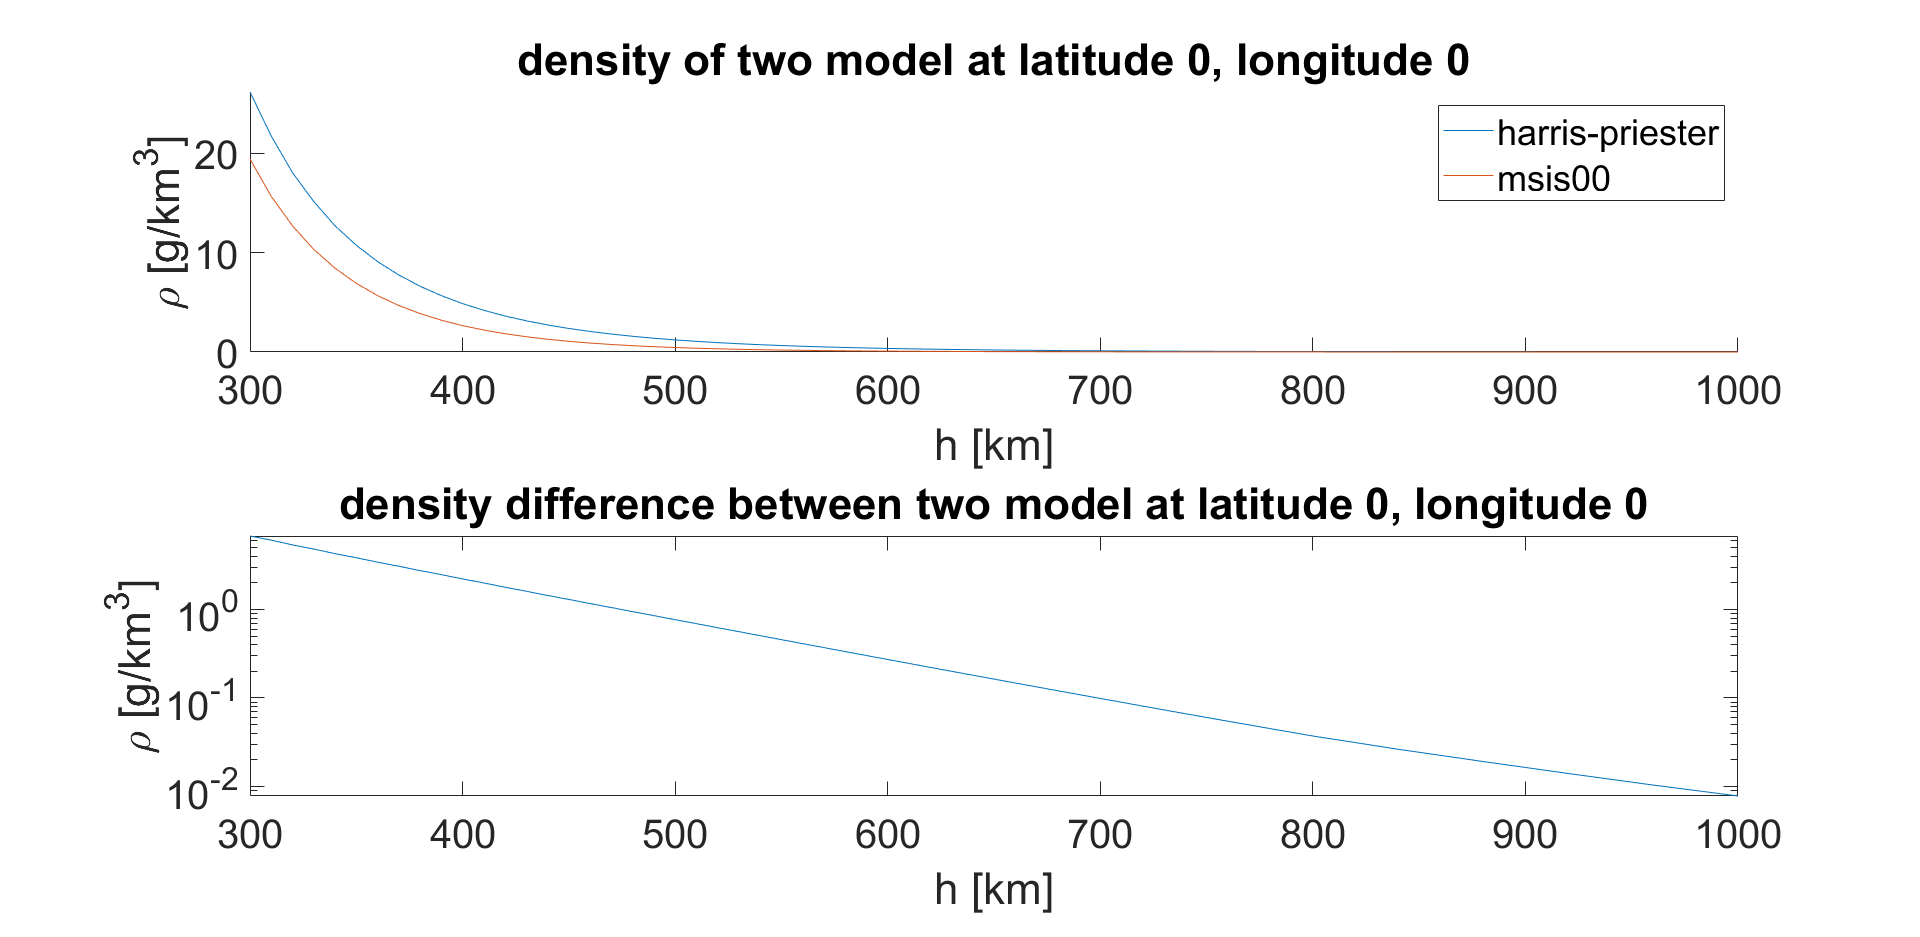
\includegraphics[width=0.9\textwidth]{images/compare_equa.png}}
	\caption{Differenzen zwischen 2 Atmosphärischen Modellen über Äquator und Nordpol}
	\label{fig:compare_model}
\end{figure}
\subsection{Andere Vereinfachung}
Satellitenbahnen werden mit nummerische Integration mit folgende Differenziale Gleichung gelöst:
\begin{equation}
	\frac{d}{dt} \begin{pmatrix}
		\bm{r} \\
		\bm{\dot{r}}
	\end{pmatrix} = \begin{pmatrix}
	\bm{\dot{r}} \\
	- \frac{GM}{r^3} \cdot \bm{r}
\end{pmatrix} + \begin{pmatrix}
\bm{0} \\
\frac{\bm{f}}{m}
\end{pmatrix}
\end{equation}
Die Störkraft $\bm{f}$ enthaltet Luftwiderstand, Solardruck usw. Da wir uns in LEO Objekten interessieren, sorgen wir nur für die atmosphärische Widerstand. Die Erde geltet als eine Kugel, daher ignoriert man die Einfluss von Erdeabplattung. Während ein Objekt um die Erde fliegt, variiert sich die Querabschnittsfläche entlang Flugrichtung wegen Kraftmoment, wir nehmen diesen Wert als einen Konstant. Die Atmosphäresgeschwindigkeit setzen wir $0$, das bedeutet, es gibt keine relative Geschwindigkeit zwischen Atmosphäre in LEO Bereich und Erde. Da wir Harris-Priester Modell verwenden, hängt die Atmosphäresdichte nur von der ellipsoidische Höhe ab, und weil wir die Erde als eine Kugel betrachtet, berechnen wir die Höhe mit folgendem Formel statt die Transformation von Kepler Elements nach Länge, Breite und Höhe zu berechnen.
\begin{equation}
	h = \lVert \bm{r} \rVert - R
\end{equation}
$R$ ist die Erdradius. Unterschiedliche Objekten haben verschiedene $C_d$ Werte, in der Simulation nehmen wir $2.5$. Danach führen wir die numerische Integration mit Hilfe von ode113 Funktion in Matlab.
\clearpage
\subsection{Integrationsergebnisse}
Wir interessieren uns die Ergebnisse unter unterschiedlichen Bedingungen. Aus \autoref{eq2} sehen wir, dass die Höhe und Verhältnis von Fläche zu Masse die Ergebnisse beeinflussen. Es ist auch offensichtlich, dass die Exzentrizität ein wichtiger Parameter ist, weil die atmosphärische Eigenschaft auf Apogäum und Perigäum sehr unterschiedlich sein könnte.
\subsubsection{Kreisbahn}
Zunächst sehen wir die einfachste Situation wenn die Exzentrizität ca. $0$ ist. Wir erhöhen die Höhe schrittweise und vergleichen die Höhenänderung. In \autoref{fig:circularorbit} sehen wir, die Objekthöhe sinkt wegen atmosphärische Widerstand. Je größer die Anfangshöhe ist, desto langsamer sinkt das Objekt wie man erwartet. Wir müssen nicht für die Objekten, deren $A/m$ gleich \SI{0,004}{\meter\squared \per \gram} sind, da sie sich in kurze Zeit automatisch abstürzen. Das Problem liegt bei den höheren Objekten. Nach 40 Jahren hat das Objekt \SI{1000}{\kilo\meter} hoch nur weniger als \SI{7}{\kilo\meter} reduziert, wobei $A/m$ schon eine große Zahl ist. Es ist offensichtlich unrealistisch, solche Objekten selber abfallen zu warten.
\begin{figure}[ht]\centering 
	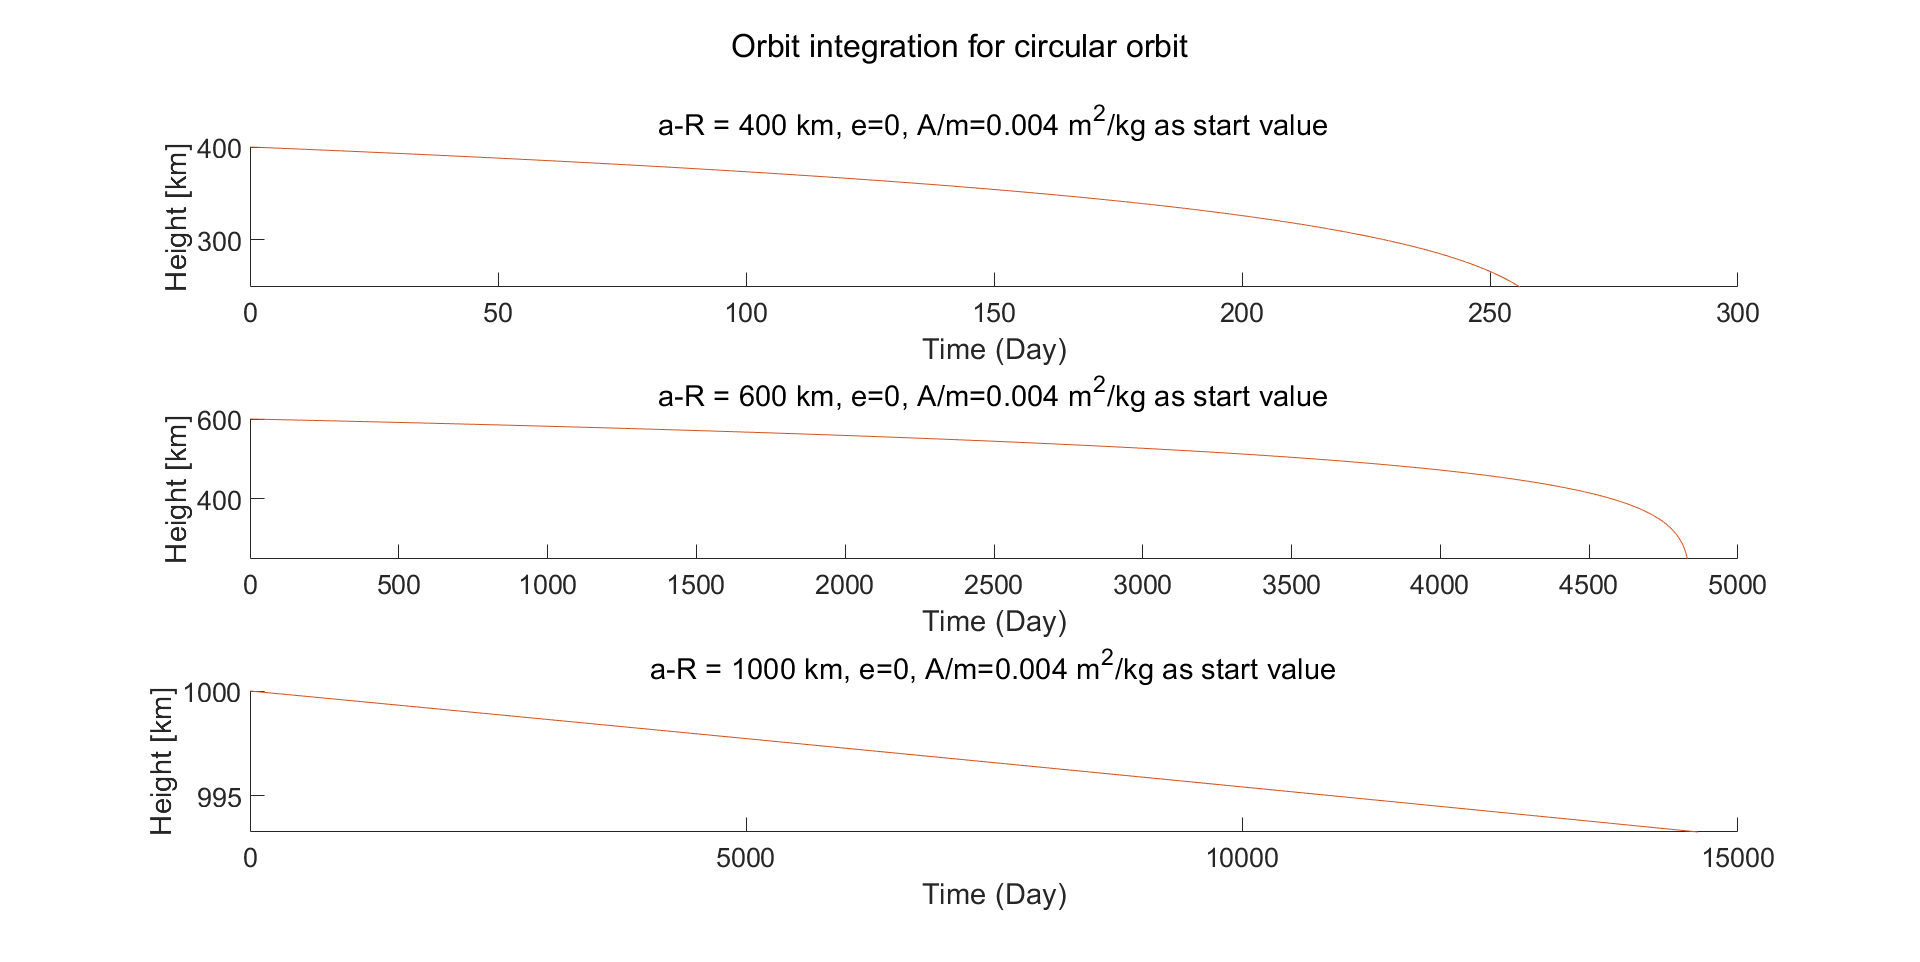
\includegraphics[width=0.8\textwidth]{images/inte_e0.png}
	\caption{Integration der Kreisbahnen von verschiedenen Höhen}
	\label{fig:circularorbit}
\end{figure}
\subsubsection{Ellipsoidische Bahnen}
Dann setzen wir die lange Halbachse fest als \SI{600}{\kilo\meter} und variieren die Exzentrizität. Die Ergebnisse is in \autoref{fig:ellipsoidalorbit} gezeigt. Das Objekt bremst sich am (nähe zu) Perigäum, da die Atmosphärische Dichte am Perigäum viel größer als die am Apogäum. Die Apogäum Höhe reduziert sich dann viel schneller als Perigäum Höhe. Diese Bahnänderung ist ähnlich wie Hohmann-Transfer, wo das Objekt sich beschleunigt, damit man die Bahnen erhöhen kann. Mit steigende Exzentrizität ist die Perigäum Höhe auch niedriger, deshalb fallt das Objekt auch schneller.
\begin{figure}[ht]\centering 
	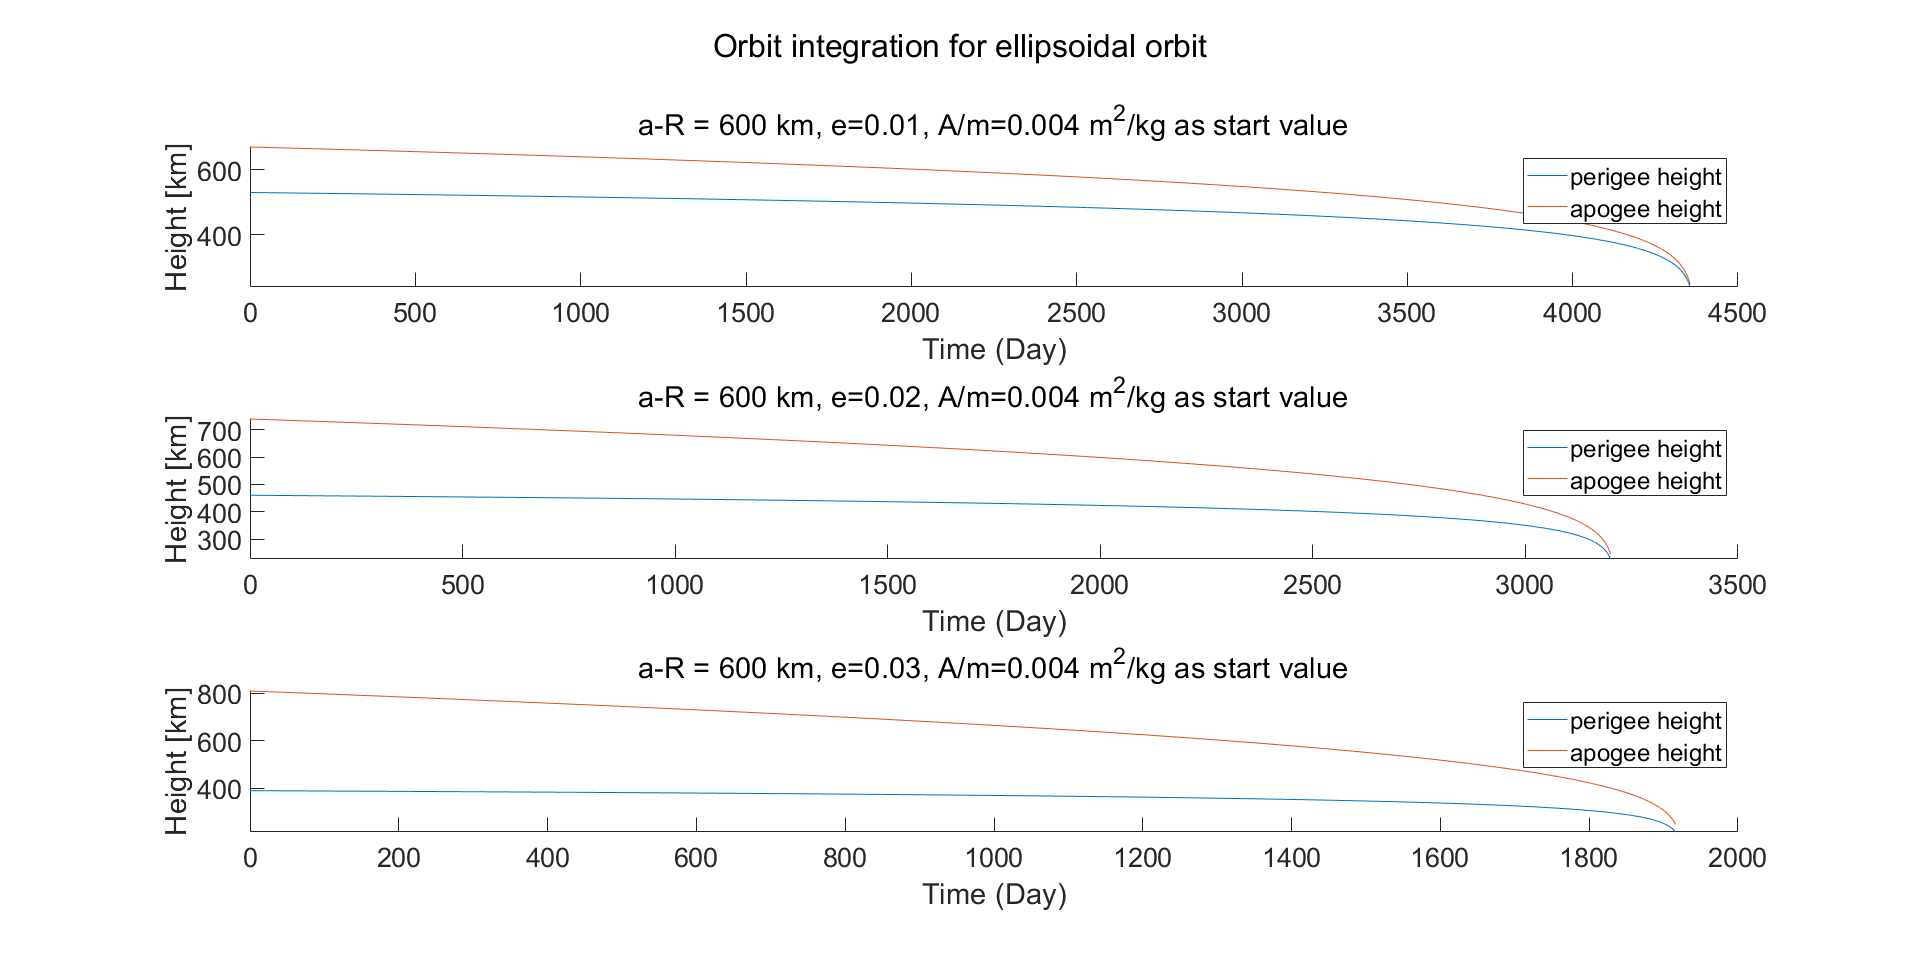
\includegraphics[width=0.8\textwidth]{images/inte_change_e.png}
	\caption{Bahintegration mit verschiedene Anfangsexzentrizität in Höhe von \SI{600}{\kilo\meter}}
	\label{fig:ellipsoidalorbit}
\end{figure}
\\\\
Ein anderer wichtiger beeinflussender Faktor ist allerdings $A/m$. Wir interessieren uns wie $A/m$ und Exzentrizität die Zeit beeinflussen, die Raumobjekt brauch, abzustürzen. Wir haben die vorherige Simulation mehrmals durchgeführt und zeigen das Ergebnis in \autoref{fig:droptime}. Entweder mit eine große Exzentrizität (obwohl 0,05 seltsam in Realität existiert) oder mit eine großer $A/m$ wird die Abfallzeit deutlich verringern.
\begin{figure}[ht]\centering 
	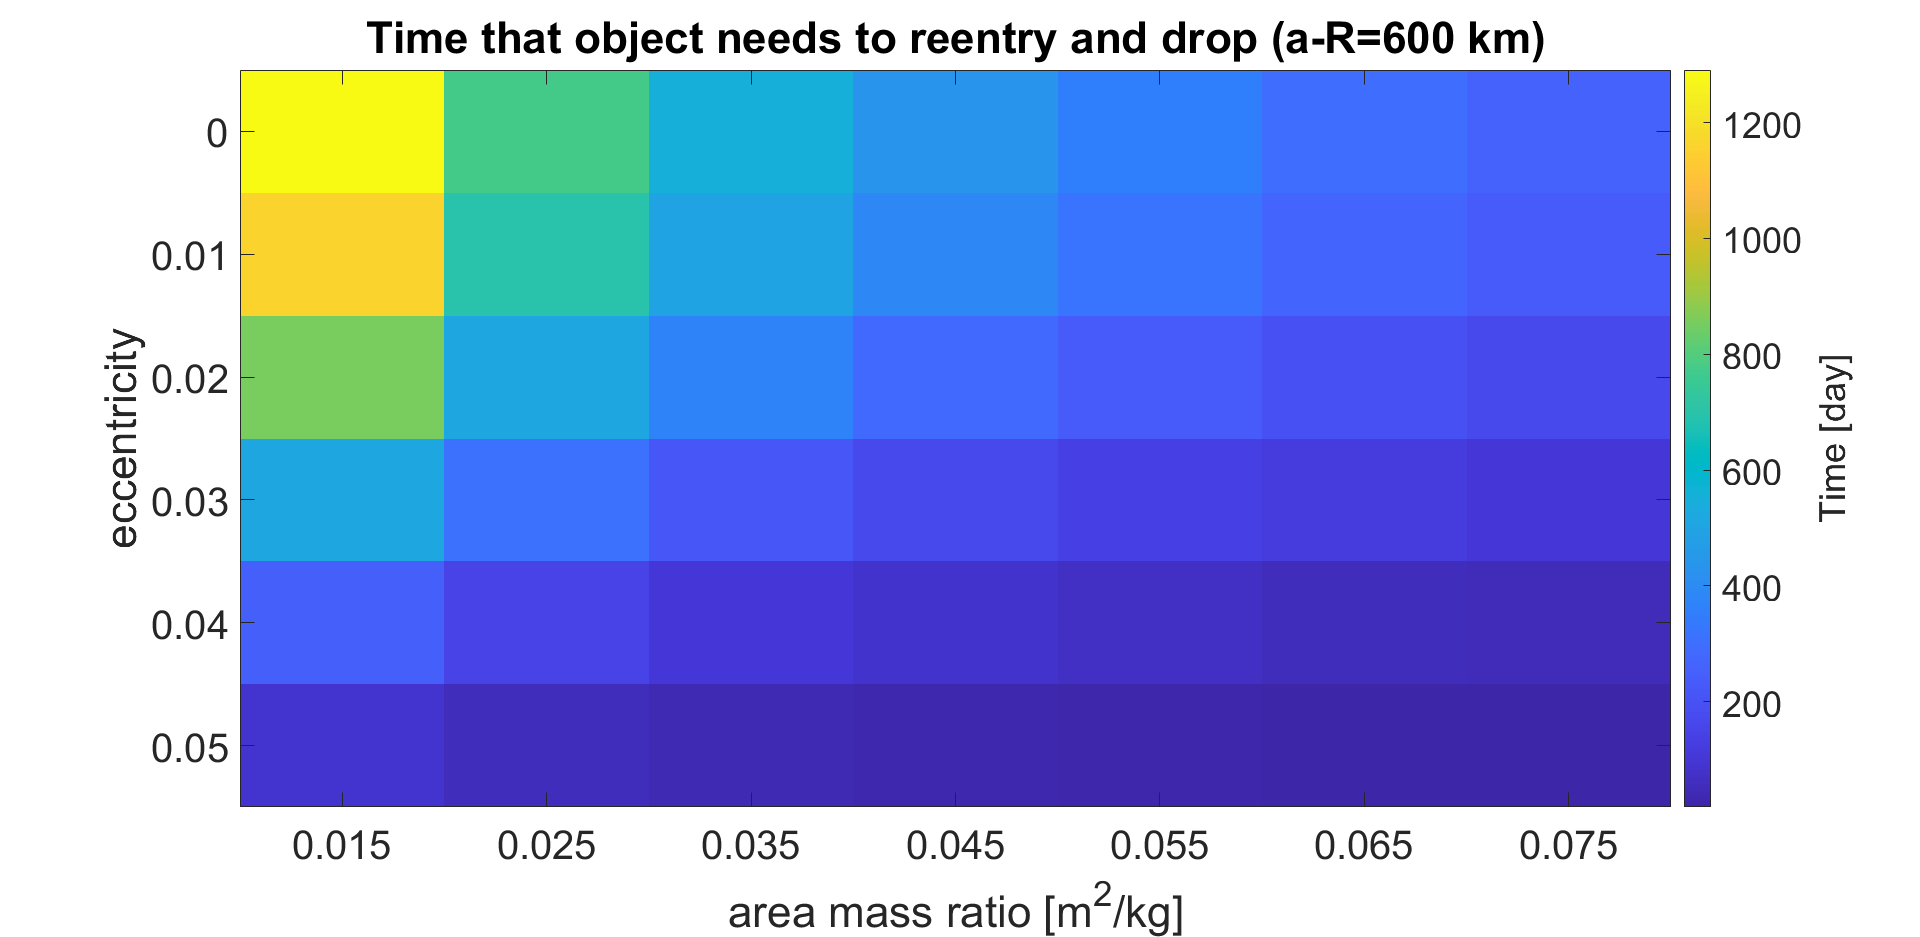
\includegraphics[width=0.78\textwidth]{images/drop_time_600.png}
	\caption{Absturzzeit mit verschiedene $A/m$ und Exzentrizität Einstellungen}
	\label{fig:droptime}
\end{figure}
\\\\
Die Realität ist leider brutal, \autoref{fig:distribution_adm} zeigt die $A/m$ Verteilung von 12472 Raumobjekten in September 2022. Meisten Objekten dargestellt sind 'Payload' und 'Rocket Body', da die Masse und Querschnitt Fläche von anderen Typen sind kaum vorhanden und schwierig zu messen. Trotzdem sehen wir, dass meisten Objekten, deren Daten vorhanden sind, haben eine kleine $A/m$, was keine positive Nachricht ist. In \autoref{fig:distribution_ae} ist die Information der lange Halbachse und Exzentrizität Verteilung. Die Objekten haben in meisten Situationen kleine Exzentrizität und gleichzeitig auch relative hohe Bahnen. Menschen müssen was gegen solche Raummüll tun statt nur warten, bis sie automatisch verschwinden. In den Kapiteln danach werden manche Ideen und Methoden diskutiert.
\begin{figure}[ht]\centering 
	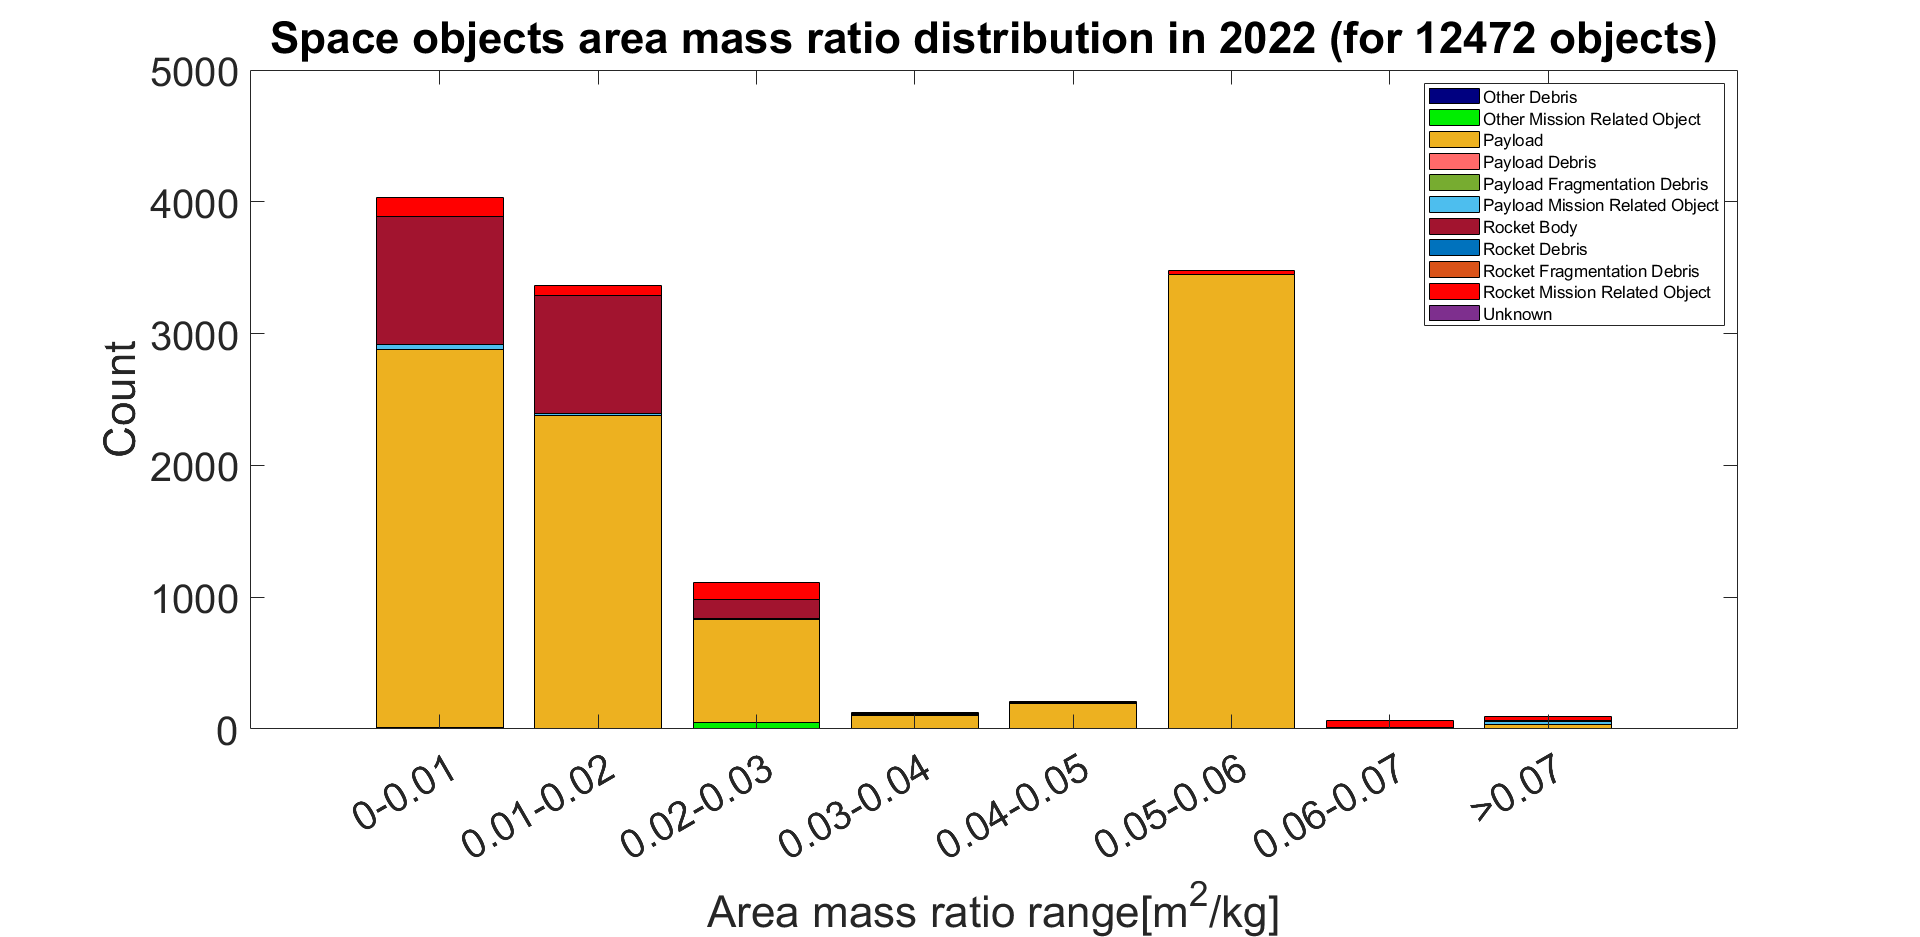
\includegraphics[width=0.9\textwidth]{images/adm_plus_classification.png}
	\caption{$A/m$ Verteilung aller Objekten in September 2022}
	\label{fig:distribution_adm}
\end{figure}
\begin{figure}[ht]\centering 
	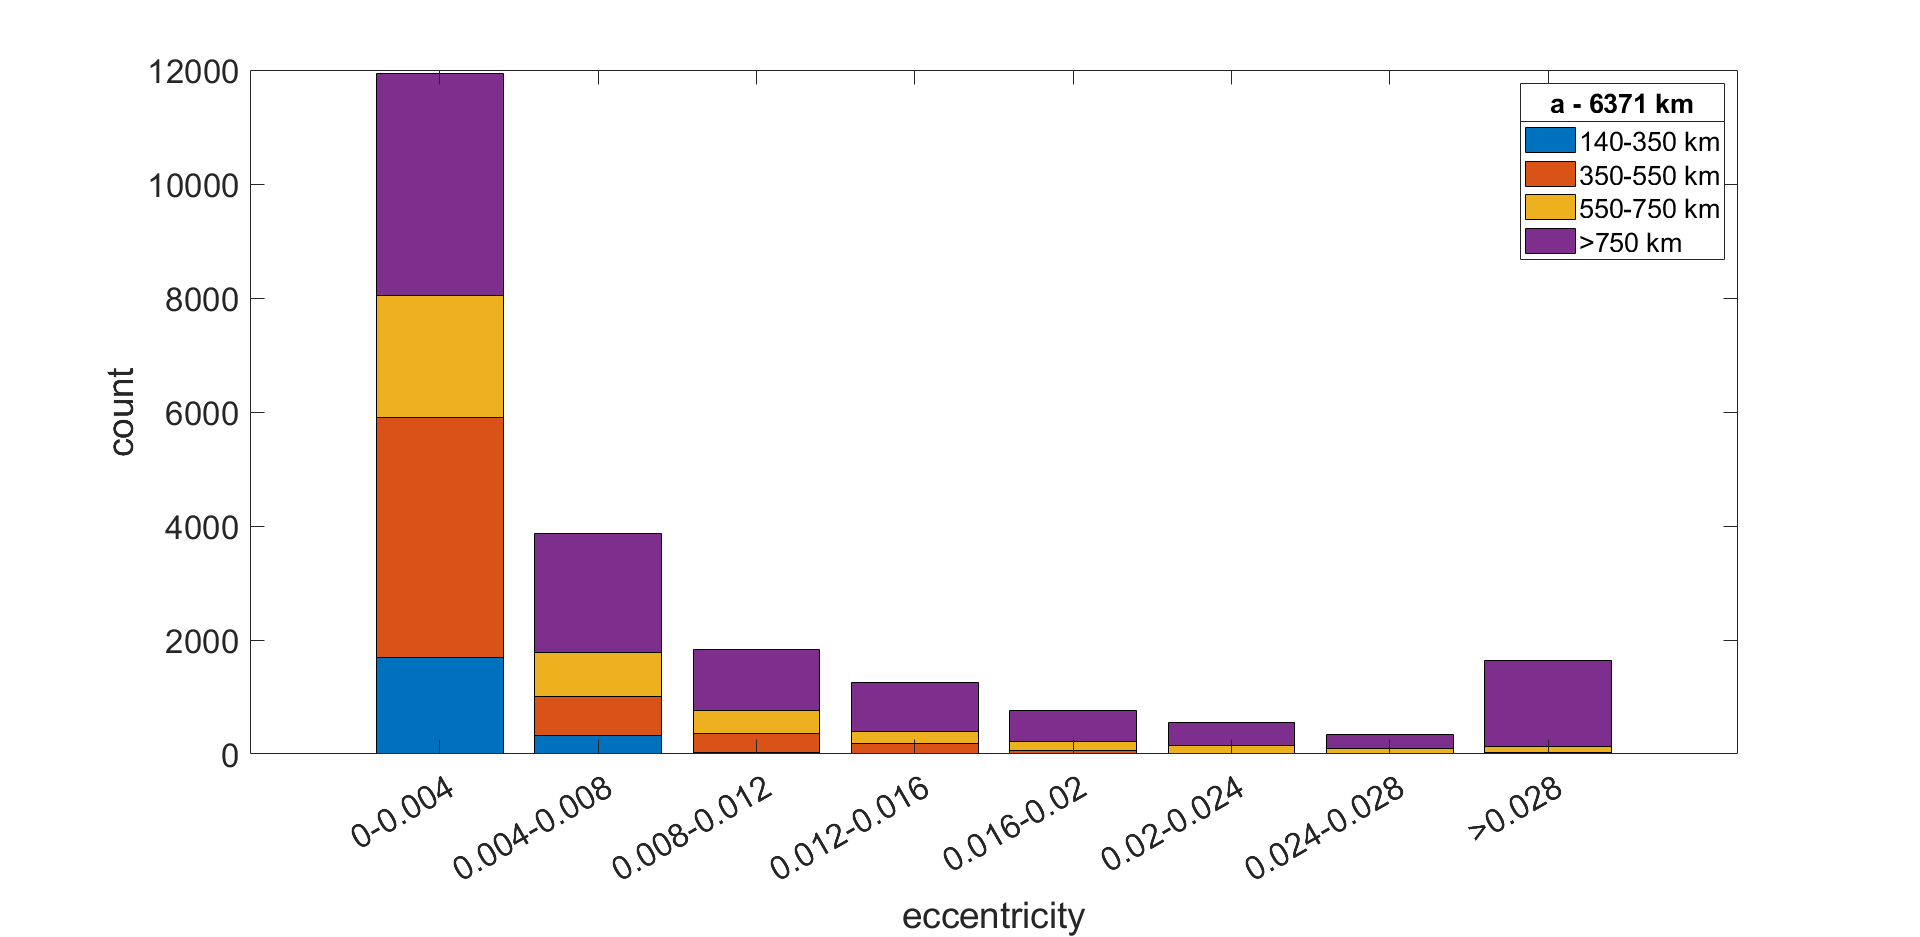
\includegraphics[width=0.9\textwidth]{images/ae_statistic.png}
	\caption{Exzentrizität Verteilung aller Objekten in September 2022}
	\label{fig:distribution_ae}
\end{figure}
\clearpage
\section{Segelbasierte Methoden}\label{sec:segel}
\subsection{DE-ORBITING SATELLITES IN LEO MIT SOLAR SAILS}
\subsubsection{Einführung und Motivation}
Die Beseitigung von Weltraumschrott ist zu einem sehr wichtigen Teil des kommerziellen und wissenschaftlichen Raumfahrtmanagements geworden. Besonders wichtig ist dies im erdnahen Orbit (Low Earth Orbit, LEO), wo es aufgrund der hohen Dichte an aktiven und inaktiven Satelliten wichtig ist, Zusammenstöße zwischen Raumfahrzeugen oder Teilen davon zu verhindern. 
\begin{figure}[htbp]
	\centering
	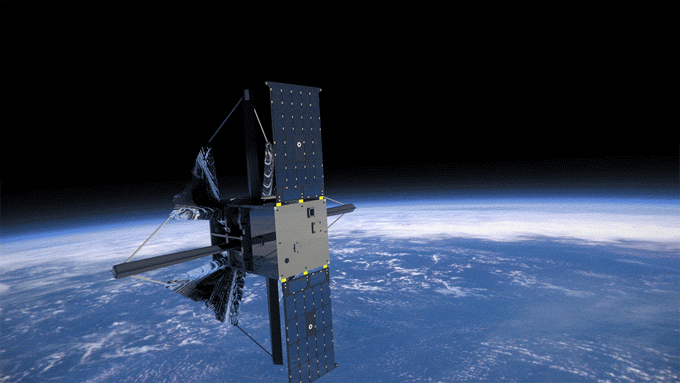
\includegraphics[width=0.7\textwidth]{bilder/Segel.png}
	\caption{Ein Bild, das zeigt, wie sich ein Sonnensegel in der Umlaufbahn um die Erde entfaltet. (Bildnachweis: NASA)}
	\label{Segel}
\end{figure}
Im Jahr 2006 unterzeichneten ASI, BNSC, CNES, DLR und ESA einen \"Europäischen Verhaltenskodex\", der eine Reihe von Vorschlägen enthält, wie die Zunahme von Weltraumschrott in den nächsten Jahren verhindert werden kann. Dieses Dokument führte im April 2008 zum ESA-Dokument "Requirements on Space Debris Mitigation for Agency Projects", das die Regeln festlegt, die von jeder zukünftigen europäischen Mission befolgt werden müssen. Nach diesen Regeln muss jeder europäische Satellit in einer Höhe von \SI{2000}{\kilo \meter} innerhalb von 25 Jahren nach dem Ende seiner Mission die Umlaufbahn verlassen. Mögliche Strategien bestehen darin, den Treibstoff an Bord zu nutzen, um am Ende der Lebensdauer des Raumfahrzeugs ein Wiedereintritt durchzuführen. Ein solcher Ansatz ist jedoch nicht durchführbar, wenn das Raumfahrzeug kein Antriebssystem an Bord hat. In diesem Fall muss eine alternative Lösung gefunden werden. Der auf Sonnensegeln basierende Ansatz erschien aus diesem Grund erstmals im Jahr 2011. \citet{Daniele:2012} erforschten den Einsatz von Sonnensegeln für das Deorbiting von Weltraumschrott. \autoref{Segel} zeigt wie sich ein Sonnensegel in der Umlaufbahn um die Erde entfaltet.

\subsubsection{Atmosphärischer Luftwiderstand}
Unter den verschiedenen Möglichkeiten und Konfigurationen stellt die Deorbitierung unter Nutzung des atmosphärischen Luftwiderstands und des solaren Strahlungsdrucks eine erste Anwendung dar. Der atmosphärische Luftwiderstand ist eine der Hauptquellen der störenden Beschleunigung für LEO-Satelliten. Diese Kraft $f_{drag}$ wird üblicherweise durch\autoref{eq2} beschrieben, mit dem Widerstandsbeiwert $C_D$, der Dichte der Atmosphäre $\rho$, dem Fläche-Masse-Verhältnis $A/m$, der Geschwindigkeit des Raumfahrzeugs $\boldsymbol{V}$ und der Geschwindigkeit der Atmosphäre $\boldsymbol{V}_{a t m}$.\\\\
Der Luftwiderstand hängt von vielen Faktoren ab, und es ist leicht zu erkennen, dass er erhöht werden kann, wenn der Wert vom Fläche-Masse-Verhältnis erhöht wird, und somit die Zeit von Deorbiting verkürzt werden kann. Der Einsatz von Sonnensegeln als Aerobraking-Geräte gegen Weltraumschrott und zur Reduzierung der Anzahl potenziell gefährlicher Objekte in der niedrigen Erdumlaufbahn ist deswegen eine Anwendung. Es ist möglich, den Wert vom Fläche-Masse-Verhältnis mit Hilfe eines Sonnensegels zu erhöhen und so das Deorbiting zu beschleunigen.
\subsubsection{Gossamer Projekt}
Das Deutsche Zentrum für Luft- und Raumfahrt (DLR) war eines der ersten Forschungszentren, das sich mit der Technologie der Sonnensegel befasst hat. Tatsächlich hat das DLR bereits im Jahr 1999 einen erfolgreichen Test zur Entwicklung eines $20\times20$ Meter großen Segels durchgeführt. Im Jahr 2010 wurden die Solarsegel-Aktivitäten wieder aufgenommen und das von der ESA geförderte Gossamer-Projekt, wurde auf dem $2^{nd}$ International Symposium on Solar Sailing in New York offiziell vorgestellt \citep{Geppert:2011}. Die im Rahmen des ESA-Projekts "Deployable Gossamer Sail for Deorbiting" durchgeführte Aktivität konzentrierte sich auf die die Reduzierung von Weltraumschrott in der LEO-Orbit. Die Aktivität bestand in der Entwicklung eines End-of-Life-Debitsystems, dem sogenannten Gossamer Deorbiter, der es neuen Raumfahrzeugen ermöglichen wird, den Europäischen Verhaltenskodex zu erfüllen \citep{FERNANDEZ:2014}.\\\\
Der erste Schritt des Gossamer-Projekts ist der Einsatz eines $5\times5$ Meter großen Sonnensegels in der Erdumlaufbahn, um die Möglichkeiten der Herstellung, der Verpackung und des erfolgreichen Einsatzes eines vollständig Systems im Weltraum zu beweisen. Die Weiterentwicklung von Gossamer-2 besteht darin, in der Erdumlaufbahn eine vorläufige Lage- und Bahnregelung zu testen. Als dritter Schritt des Programms, Gossamer-3, ist schließlich eine interplanetare Mission in vollem Umfang geplant.
\subsubsection{Vorbereitung auf die Simulation}
Um die Möglichkeit des Einsatzes von Sonnensegeln zu untersuchen, wurden Simulationen in Matlab durchgeführt und die Ergebnisse mit denen aus dem Papier von \citet{Daniele:2012} verglichen. \\\\
Die Untersuchung der Auswirkungen des atmosphärischen Luftwiderstands auf ein Raumfahrzeug ist eine der größten Herausforderungen bei der Simulation. Von den bereits erwähnten Harris–Priester - und MSIS-Modellen ist das MSIS-Modell zwar genauer, aber aufgrund des riesigen Zeitaufwands mussten wir es zugunsten des effizienteren Harris–Prieste Modells aufgeben. Auf dieser Grundlage wurden die Keplerschen Elemente der Satellitenbahn in Matlab simuliert, wobei ODE113 zur Integration verwendet wurde. \\\\
Neben der Umlaufbahn des Satelliten beeinflusst die Attitude des Sonnensegels den Luftwiderstand. Aufgrund der Komplexität der Attitude-lösung haben wir dies in den Matlab-Simulationen jedoch nicht berücksichtigt, sondern sind davon ausgegangen, dass die Orientierung des Sonnensegels zu jedem Zeitpunkt konstant ist, was natürlich nicht der Realität entspricht. In gewisser Weise gehen wir davon aus, dass das aerodynamische Drehmoment stark genug ist, um eine passive Stabilisierung zu gewährleisten, wie wir später noch genauer erläutern werden. \\\\
Unser Testszenario berücksichtigt die folgenden Bedingungen:
\begin{itemize}
	\item Orbit: \SI{600}{\kilo\meter} Höhe
	\item Gesamtmasse des Satelliten: \SI{2500}{\kilo\gram} / \SI{500}{\kilo\gram}
	\item Segelfläche: \SI{25}{\square \meter}
\end{itemize}
\subsubsection{Analyse der Ergebnisse}
\begin{figure}[H]
	\centering
	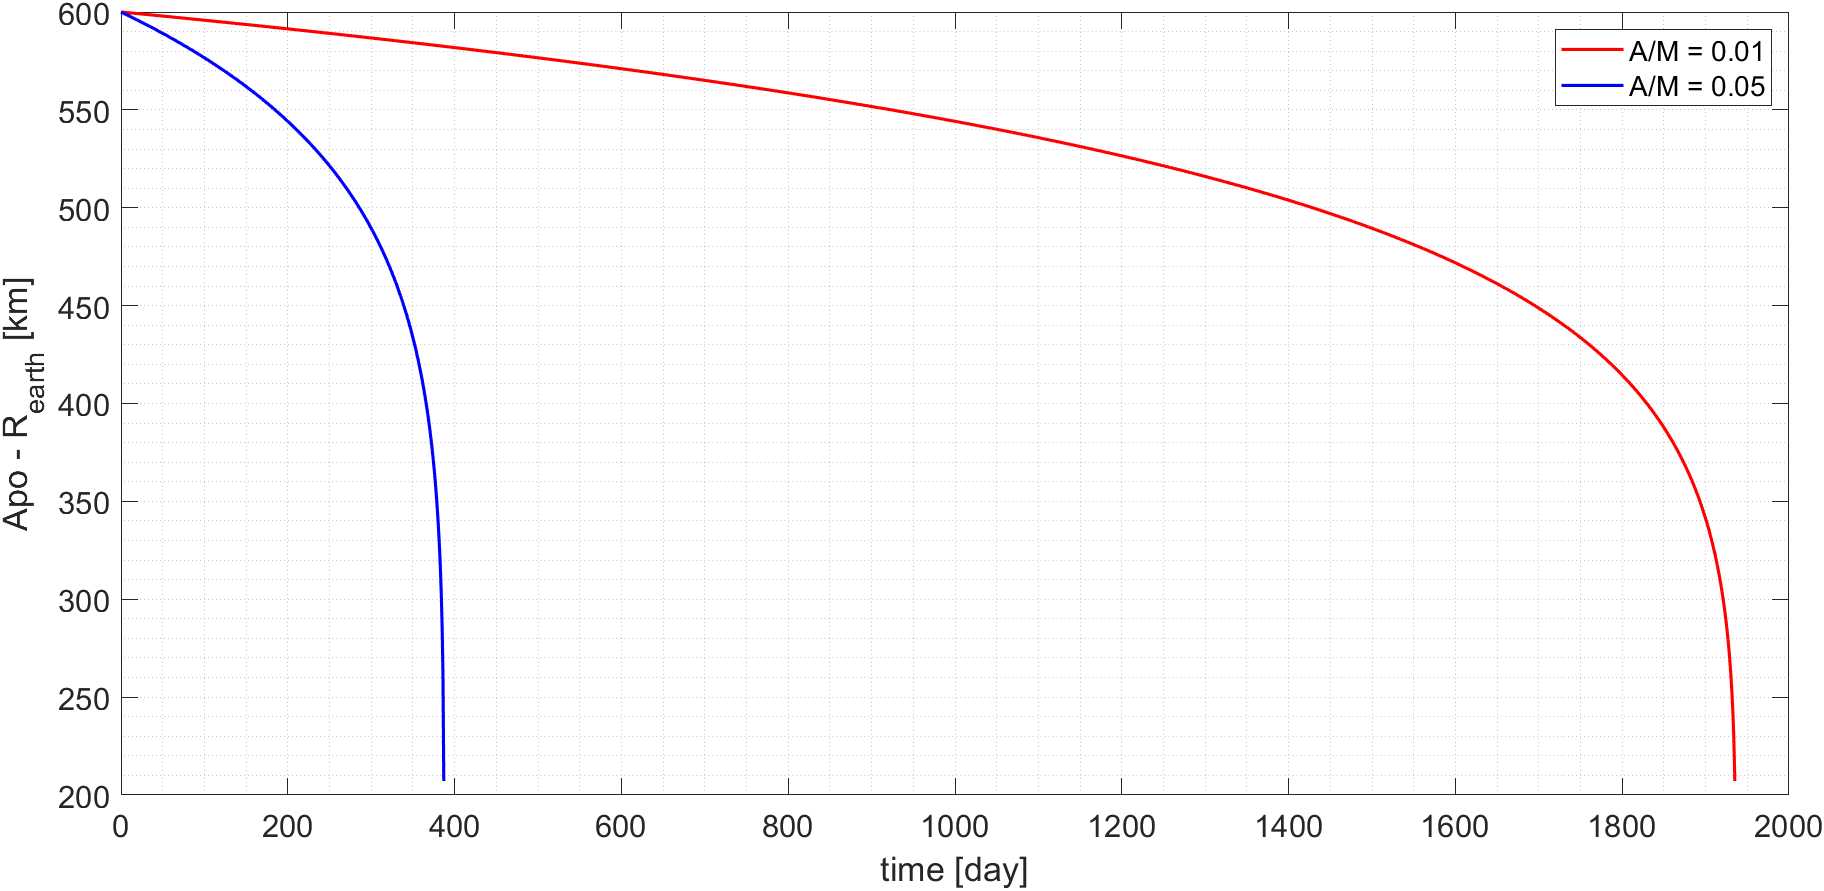
\includegraphics[width=0.7\textwidth]{bilder/Simulation_Matlab.png}
	\caption{Ergebnisse der Simulation in Matlab: Änderung der Höhe des Apogäums mit der Zeit nach Abzug des Erdradius, wobei rot das Ergebnis eines $A/M$ von 0,01 und blau das Ergebnis eines $A/M$ von 0,05 ist.}
	\label{Simulation_Matlab}
\end{figure}
Die Ergebnisse der Simulation in Matlab sind in \autoref{Simulation_Matlab} dargestellt. Wir haben zwei verschiedene $A/M$ ausprobiert, die mit ODE113 berechnet wurden, um die Veränderung der Apogäumshöhe über die Zeit nach Abzug des Erdradius zu ermitteln. Die Simulation zeigt, dass das Raumfahrzeug im Testszenario mit $A/M$ = 0,05 in etwa 2000 Tage wieder in die Atmosphäre eintritt: Es ist zu beachten, dass der Satellit als wieder in die Atmosphäre eingetreten gilt, wenn es eine Höhe von \SI{150}{\kilo\meter} über dem Geoid erreicht. Das ist sicherlich nicht ideal, aber wenn das $A/M$ um den Faktor fünf erhöht wird, verkürzt sich die Zeit signifikant auch um einen Faktor von fast fünf.
\begin{figure}[H]
	\centering
	\includegraphics[width=0.6\textwidth]{bilder/Simulation_paper.png}
	\caption{Höhe des Satelliten über dem Geoid im Laufe der Zeit mit einer Orbithöhe von \SI{450}{\kilo\meter},  Gesamtmasse von \SI{140}{\kilo\gram} und einer Segelfläche von \SI{25}{\square \meter}}
	\label{Simulation_paper}
\end{figure}
Das erste Testszenario in dem Papier verwendet unterschiedliche Bedingungen: 
\begin{itemize}
	\item Orbit: \SI{450}{\kilo\meter} Höhe
	\item Gesamtmasse des Satelliten: \SI{140}{\kilogram}
	\item Segelfläche: \SI{25}{\square \meter}
\end{itemize}
\autoref{Simulation_paper} zeigt nicht die Apogäumshöhe, sondern die Bahnhöhe, und die Schwankungen im Bild sind auch auf die elliptische Bahn zurückzuführen. Obwohl die Szenarien unterschiedlich sind, zeigen unsere Simulationsergebnisse und die Ergebnisse im Papier ähnliche Trends. Mit einem $A/M$ von ca. 0,18 wurde die Bahnhöhe in nur 20 Tagen von 450 km auf 150 km reduziert. Die vorläufigen Schlussfolgerung ist, dass die Verwendung eines Sonnensegels kann daher nützlich sein. 
\\\\
Weitere Untersuchungen müssen jedoch in einem allgemeineren Rahmen durchgeführt werden, um festzustellen, in welcher Höhe die Ausleger des Sonnensegels nicht mehr in der Lage sind, die aerodynamischen Drehmomente zu bewältigen, was zum Zusammenbruch der Struktur führt. Wie bereits erwähnt, ist die Ausrichtung des Sonnensegels entscheidend, denn eine stabile Orientierung ist notwendig, um eine stabile Querschnittsfläche und den Luftwiderstand zu gewährleisten, was in unseren Simulationen nicht berücksichtigt wird. Da in das Papier wurde die Attitude des Sonnensegels zusammen mit der Bahnbewegung berücksichtigt, ist es möglich, den Querschnitt in Bezug auf die Atmosphäre über die Zeit während der Simulation darzustellen (Siehe \autoref{Attitude_Paper}).
\begin{figure}[htbp]
	\centering
	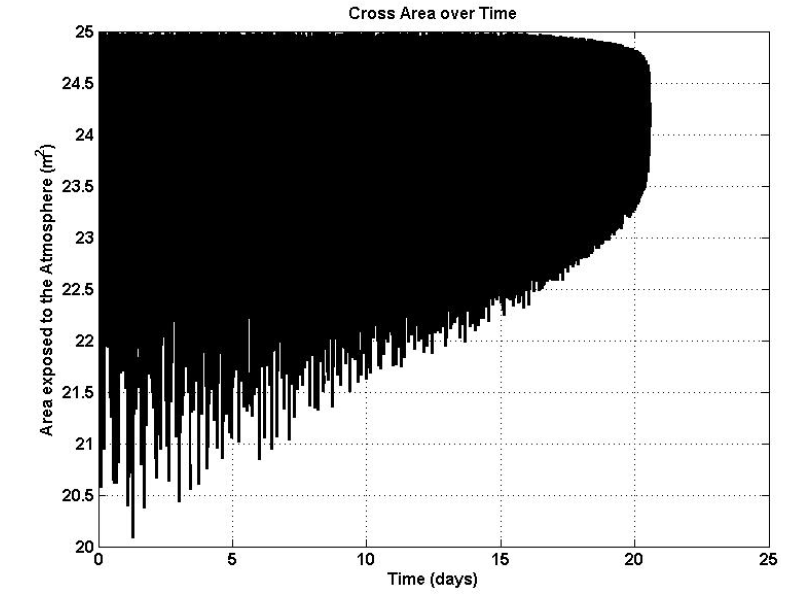
\includegraphics[width=0.7\textwidth]{bilder/Attitude_Paper.png}
	\caption{Querschnittsfläche über die Zeit}
	\label{Attitude_Paper}
\end{figure}
Es ist klar, dass das aerodynamische Drehmoment, das auf dem Sonnensegel wirkt, stark genug ist, um eine passive Stabilisierung zu gewährleisten, wobei das Segel wie ein Fallschirm wirkt und der verdünnten Atmosphäre eine konstante Fläche von etwa \SI{24}{\square \meter} bietet. Aufgrund des aerodynamischen Drehmoments wird der Luftwiderstand des Segels kostenlos maximiert ohne eine aktive Steuerung. Es ist aber wichtig zu beachten, dass diese passive Stabilisierung nur erreicht werden kann, wenn das aerodynamische Drehmoment stark genug ist. 
\begin{figure}[htbp]
	\centering
	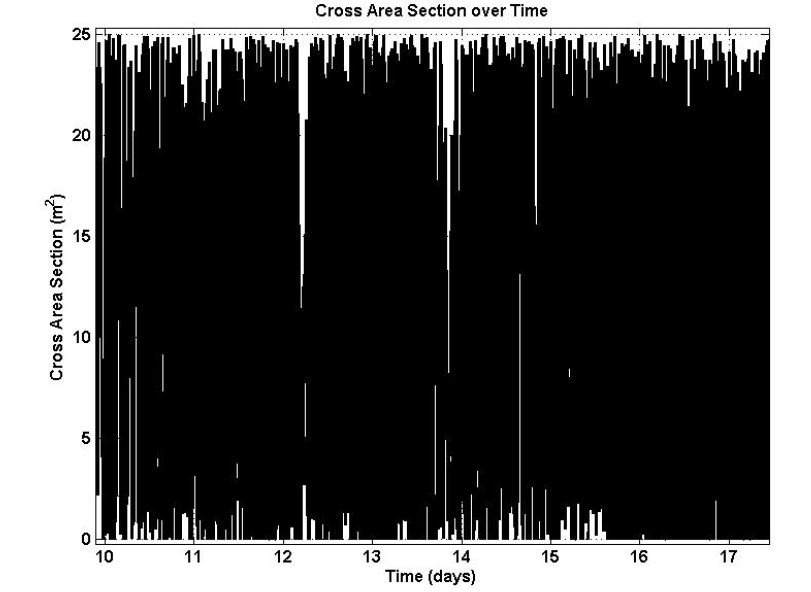
\includegraphics[width=0.7\textwidth]{bilder/Attitude2_Paper.png}
	\caption{Querschnitt über die Zeit (detaillierte Ansicht eines Zeitraums von einer Woche) mit einer Bahnhöhe von \SI{600}{\kilo\meter},  Gesamtmasse von \SI{140}{\kilogram} und einer Segelfläche von \SI{25}{\square \meter}}
	\label{Attitude2_Paper}
\end{figure}
Die Situation wird nicht optimal, wenn die Bahnhöhe ansteigt. Neue Simulationen mit einer Bahnhöhe von \SI{600}{\kilo\meter} zeigt, dass die gewünschte "passive Stabilisierung" zur Maximierung der Fläche kann nicht mehr erreicht werden. Das liegt daran, dass das verfügbare aerodynamische Drehmoment nicht ausreicht, um die Rotation des Satelliten auszugleichen. Tatsächlich ist die atmosphärische Dichte in \SI{600}{\kilo\meter} Höhe um ein bis zwei Größenordnungen geringer als in \SI{450}{\kilo\meter} km Höhe, was gemäß Gleichung \autoref{eq2} zu einer viel geringeren Widerstandskraft führt. Das bedeutet, dass die Situation, die wir in Matlab simulieren, in der Realität nicht realisierbar ist. In \autoref{Attitude2_Paper} ist es zu sehen, dass der Satellit erheblich taumelt, was zu einer Querschnittsfläche im gesamten Bereich zwischen \SI{0}{\square \meter} und \SI{25}{\square \meter} führt.
\subsubsection{Zusammenfassung}
In diesem Abschnitt wurde die Möglichkeit untersucht, ein Sonnensegel für das Deorbiting in der LEO-Orbit zu verwenden. Es wurden die theoretischen Grundlagen für die Simulation einer solchen Anwendung erläutert und die wichtigsten Probleme beschrieben, die bei dieser Aufgabe auftreten können. Die vorläufige Analyse hat gezeigt, dass die Verwendung eines Sonnensegels unter bestimmten Einschränkungen nützlich sein. Für die Realisierung dieses Verfahrens sind natürlich detailliertere Versuchsdaten erforderlich.

\subsection{DE-ORBITING SATELLITES IN LEO USING SOLAR SAILS}
\subsubsection{Einführung}
Der solare Strahlungsdruck ist die Störung, die durch die Wechselwirkung zwischen den von der Sonne kommenden Photonen und der äußeren Oberfläche des Satelliten entsteht. Obwohl Sonnensegel auf solche Wechselwirkungen angewiesen sind, um Schub zu erzeugen, ist diese Wechselwirkung eine Störung für Satelliten in der LEO-Orbit und haben um mehrere Größenordnungen weniger Wirkung als andere. Für höhere Umlaufbahnen, wie z.B. geosynchrone Umlaufbahnen, bietet der solare Strahlungsdruck aber eine einzigartige Lösung, um größeren Weltraumschrott zu entfernen. \\\\
Nach dem aktuellen Stand der Technik kann ein CubeSat mit einem Hochleistungs-Sonnensegel als Antrieb Satelliten in der Größenordnung von \SI{1000}{\kilogram} deorbitieren. Dieser CubeSat, auch "TugSat" genannt, wird in der Studie von \citet{Kelly:2018} simuliert und einen Satelliten virtuell aus der geostationären Umlaufbahn ohne den Einsatz von Standard-Antriebssystemen deorbittet. Dieser TugSat kann zwischen dem geostationären Orbit und dem Friedhofsorbit wiederverwendet werden, um kontinuierlich Schrott aus den wertvollen geostationären Umlaufbahn zu entfernen. Das gesamte Deorbit-Manöver wird die Kontrolle über die Halbachse des Sateliten, die Exzentrizität, die Inklination darstellen: alles unter Verwendung von Techniken zur Optimierung der zeitlichen Änderungsraten der Bahnelemente des Satelliten. 
\subsubsection{Kraft aufgrund von Solardruck}
Die Formel für die Kraft, die durch den Strahlungsdruck der Sonne entsteht, lautet wie folgt:
\begin{equation}
	\boldsymbol{f}=-\kappa P_{\odot} \frac{A U^2}{r_{\odot}^2} \frac{A}{m} \cos \theta\left[(1-\varepsilon) \hat{\boldsymbol{r}}_{\odot}+2 \varepsilon \cos \theta ~\widehat{\boldsymbol{n}}\right]
\end{equation}
\begin{itemize}
	\item $P_{\odot}$: Größenordnung des solaren Strahlungsdrucks
	\item $r_{\odot}$: die Distanz zum Satelliten
	\item $AU$: die astronomische Einheit
	\item $\kappa$: der Schattenkoeffizient
	\item $\epsilon$: der Reflexionskoeffizient
	\item $\frac{A}{m}$: das Flächen-Masse-Verhältnis
	\item Winkel $\theta$ zwischen dem Sonnenrichtungsvektor $\hat{\boldsymbol{r}}_{\odot}$ und der Segelflächennormale $\widehat{n}$
\end{itemize}
Unter einigen Annahmen, ${AU}^2\approx1,~\kappa=1,~\epsilon=1$, kann eine charakteristische Kraft definiert werden als:
\begin{equation}
	\ddot{\boldsymbol{r}}_{\mathrm{SRP}} \approx-a_c \cos ^2 \theta ~\hat{\boldsymbol{n}}, \quad \theta \in\left[0, \frac{\pi}{2}\right]
	\label{SRP}
\end{equation}
Aus Gleichung \autoref{eq2} geht hervor, dass die Größe des solaren Strahlungsdrucks direkt von der Richtung der Normalen der Segeloberfläche abhängt. \\\\
Die Simulation basiert auf einem \SI{50}{\kilogram} schweren Satelliten, der mit einem perfekt reflektierenden, \SI{800}{\square \meter} (ca. $28 \times \SI{28}{\square \meter}$) großen Sonnensegel ausgestattet ist. Mit der zusätzlichen Masse einer \SI{1000}{\kilogram} schweren Nutzlast beträgt das Flächen-Masse-Verhältnis des Gesamtsystems \SI{0.76}{\square \meter \per \kilogram}.

\subsubsection{TugSat}
Die TugSat-Simulation soll das Potenzial zeigen, mit einem Sonnensegelsatelliten Weltraumschrott aus dem GEO-Orbit zu entfernen. TugSat wird in einer  Umlaufbahn innerhalb des GEO-Orbits gestartet und beginnt damit, die Hauptachse seiner Umlaufbahn um \SI{350}{\kilo\meter} anzuheben. Sobald das Ziel der semimajoralen Achse erreicht ist, wird TugSat die Exzentrizität seiner neuen Umlaufbahn verringern und dabei eine Höhe für Friedhofsumlaufbahnen beibehalten. Als Nächstes lässt TugSat die Nutzlast los und beginnt mit dem Abstieg zurück in den GEO-Orbit.
Diese Manöver werden unter Verwendung der optimierten Segelausrichtung durchgeführt.
\subsubsection{Simulation}
Nachdem die primären Manöver beschrieben wurden, kann die gesamte TugSat-Simulation dargestellt werden. 
Das erste Ziel beim Deorbit mit TugSat ist es, die Hauptachse der Nutzlast zu vergrößern. TugSat wird die Nutzlast deorbitieren, indem es das Apogäum erhöht und die Halbachse \SI{350}{\kilo\meter} über dem GEO-Orbit anhebt. Sobald die gewünschte Halbachse erreicht ist, verringert TugSat die Exzentrizität der Umlaufbahn, bevor es die Nutzlast freilässt. Nach der Freigabe der Nutzlast kehrt Tugsat in den GEO-Orbit zurück und peilt seine ursprüngliche Länge vom Beginn der Simulation an. \autoref{Simulation_TugSat} zeigt die TugSat-Simulation. TugSat deorbiert erfolgreich und lässt seine Nutzlast in weniger als einem Jahr frei. In weniger als anderthalb Jahren kehrt TugSat erfolgreich zum GEO-Orbit zurück. In weniger als zwei Jahren nach Beginn des Deorbit-Manövers reduziert TugSat die Bewegung auf weniger als \SI{5}{\kilo\meter}, während die Werte für die Hauptachse, die Exzentrizität konstant bleiben.

\begin{figure}[htbp]
	\centering
	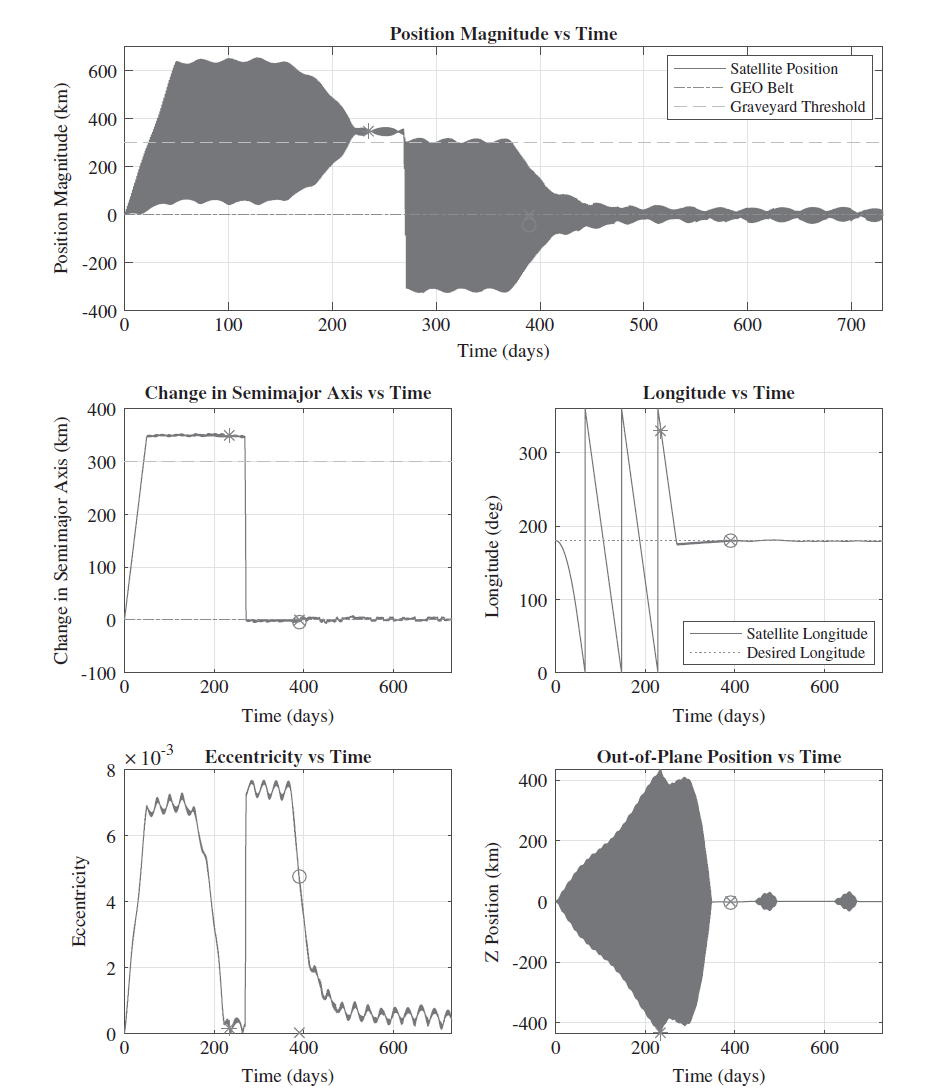
\includegraphics[width=0.8\textwidth]{bilder/Simulation_TugSat.png}
	\caption{TugSat-Simulationsergebnisse: Der Stern steht für die Freigabe der Nutzlast}
	\label{Simulation_TugSat}
\end{figure}

\subsection{Zusammenfassung}
Der solare Strahlungsdruck ist eine wichtige Ressource für Satelliten in hoch gelegenen Umlaufbahnen, insbesondere in der geostationären Umlaufbahn, und bietet eine Möglichkeit für niedrigpräzise, unbegrenzte Satellitenmanöver. Es ist noch mehr Forschung nötig, um diese Idee in Zukunft tatsächlich umzusetzen.


\section{Satellitenbasiert Methoden}\label{sec:sate}
Eine der vielversprechendsten und am weitesten entwickelten Konzepte zur Beseitigung von Raumschrott ist die satelliten-basierte. Hierbei wird eine neue "Verfolger"-Plattform in den Weltraum geschossen und von dieser aus, z.B. durch Einfangen, ein Schrottteil aus seiner Bahn entfernt. Im Folgenden wird ein typischer Missionsablauf einer satelliten-basierten Raumschrott-Entfernungs-Mission vorgestellt. In den weiteren Abschnitten werden einzelne Abschnitte der Missionen genauer beleuchtet und jeweils verschiedene Alternativen diskutiert.

\subsection{Missionsablauf}
Der hier vorgestellte Ablauf bildet eine Multi-Debris-Mission für mittelgroße Teile im LEO, z.B. mit einer Höhe von 800 km und Masse von 100 kg, dar. Das bedeutet, es werden mehrere Teile in einer Missionen und mit einer einzigen Plattform entfernt. Eine solche Art der Mission wird in Zukunft aufgrund der großen Zahl an Müllpartikeln und den Kosten für jeden Satelliten-Start unausweichlich sein. Es gibt allerdings noch Herausforderungen wie das Aufbewahren mehrerer Schrottteile in der Plattform, weshalb bislang erst eine Single-Debris-Mission in Aussicht ist (siehe \autoref{aktuell}). \\\\
Eine Satelliten-basierte Raumschrott-Entfernungs-Mission besteht im Allgemeinen aus 5 Phasen \citep{ruggiero2015small}: \\\\
\textbf{1. Start}: Es wird ein erstes Ziel der Mission ausgewählt und die Plattform auf einen Orbit nahe diesem geschossen. Das Vehikel muss sich unter und hinter seinem Ziel befinden. Durch die niedrigere Flughöhe holt der Satellit auf und nähert sich dem Ziel. Diese Annäherung wird Phasing genannt und funktioniert mit absoluter Navigation. Das bedeutet, die Position des Schrottteils ist durch TLE-Daten auf wenige Kilometer genau bekannt. Die Position der Plattform wird mit GPS bestimmt. Das Annähern läuft aufgrund der Bahnmechanik bogenförmig ab (siehe  \autoref{rendez-vous}), wie in \autoref{Rendezvous} zu sehen. Durch Schübe in along-track Richtung wird die lange Halbachse schrittweise der des Ziels angepasst. \\\\
\textbf{2. Rendez-vous} \citep{castronuovo2011active}: Das far-range rendez-vous beginnt, wenn sich die Plattform durch das Phasing genug genähert hat, je nach Definition z.B. 5 km hinter dem Ziel. Positionsbestimmung funktioniert nun mit relativer Navigation; Mit Kameras mit optischen und Infrarot-Kanälen wird die Richtung, Entfernung und Entfernungsänderung des Objekts bestimmt.\\
\begin{figure}[H]
	\centering
	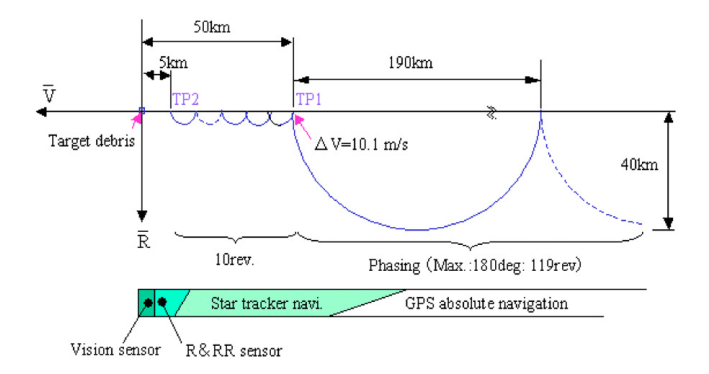
\includegraphics[width = 0.9\textwidth]{bilder/Rendezvous.png}
	\caption{Darstellung des Phasing und Rendez-vous \citep{nishida2009space}}
	\label{Rendezvous}
\end{figure}
\noindent An einem Sicherheitspunkt, wenige Meter vom Objekt entfernt, beginnt das close-range rendez-vous: Die Bewegung des Schrottteils wird geschätzt. Es wird von allen Seiten inspiziert und von einem Nahfeld-Laser kartiert ("fly-around"). \\\\
Der Satellit muss sich der Rotation des Teils bis auf weniger °/s anpassen. Für das Treffen nähert sich der Satellit in einer geraden Linie entlang der Rotationsachse des Ziels an. Dann kann der Kontakt hergestellt werden. Dabei wird die verbleibende relative Rotation abgebaut. Der Kontakt funktioniert z.B. mit einem Roboterarm, der zunächst locker eingestellt ist und dann fester wird und damit die Rotation langsam verringert. An Raketenstufen gibt es passende Greifpunkte, an denen der Arm das Teil berühren kann. Sonst muss anhand der vorherigen Inspektion ein solcher Punkt gefunden werden. Andere Möglichkeit der Kontaktnahme sind Netze oder Harpunen (siehe \autoref{Verbindung}). Schließlich wird die Formation stabilisiert, bevor sie mit den weiteren Manövern fortfahren kann. \\\\
\textbf{3. De-orbiting}: Durch das Antriebs-System der Plattform wird die Formation abgebremst und damit die Höhe verringert. Ist ein Orbit erreicht, auf dem ein Körper in absehbarer Zeit (Monate bis wenige Jahre) durch die Luftreibung in die Atmosphäre eintreten wird, kann das Schrottteil freigegeben werden. \\\\
\textbf{4. Bewegung zu weiterem Ziel}: Durch eine Reihe von Orbit-Manövern nähert sich der Satellit dem nächsten Ziel. Dabei muss die lange Halbachse und die Inklination entsprechend angepasst werden. Weiterhin muss der RAAN verändert werden. Bei letzterem kann Treibstoff gespart werden, indem der natürliche RAAN Drift ausgenutzt wird. Das bedeutet, der Satellit begiebt sich zunächst auf einen Zwischen-Orbit mit einer anderen RAAN-Driftrate und wartet dort, bis sich sein RAAN dem des Zielteils genähert hat; Danach werden Inklination und lange Halbachse angeglichen. Hat der Satellit den richtigen Orbit erreicht, wird das nächste Rendez-vous eingeleitet und die Schritte wiederholen sich. \\\\
\textbf{5. Selbstensorgung}: Am Ende der Mission, wenn z.B. nicht mehr genügend Treibstoff verfügbar ist, nutzt der Satellit sein Antriebs-System, um seine Höhe zu verringern, sodass eine Lebensdauer von unter 25 Jahren verbleibt. \\\\
Für die meisten weiteren Arten von Müllteilen muss dieses Konzept nur leicht modifiziert werden. Für größere Teile mit mehreren Tonnen Masse wird mehr Treibstoff zum Abbremsen sowie eventuell eine größere Verfolger-Plattform benötigt, damit das Ziel richtig gesichert und stabilisiert werden kann. Kleinere Teil mit Massen von g bis wenige kg gibt es im LEO um Größenordnungen mehr als schwerere ganze Satelliten oder Raketenstufen. Eine Mission zur Beseitigung solcher Teile müsste viele Teile auf einmal beseitigen können, um effektiv zu sein. Dazu müssten Teile im Inneren der Plattform abgelegt werden können, bevor das Vehikel nach weiteren Teilen sucht und erst nach einer bestimmten Gesamtmasse das De-orbiting einleitet. Zum Einfangen wäre ein engmaschiges Netz (siehe \autoref{Verbindung}) geeignet, da ein Roboterarm diese kleinen Partikel nicht greifen kann. Aufgrund der großen Anzahl solcher kleinen Teile dürfte zu diesem Ziel aber eine Laser-basierte Mission (siehe \autoref{sec:laser}) zu bevorzugen sein. Für diese wird eine geringere Impulsänderung benötigt, das heißt der Laser kann in einem Überflug das De-orbiting des Teils einleiten. \\\\
Bei Müllteilen im geostationären Orbit muss ein Abstellorbit gewählt werden, in der keine arbeitenden Staelliten gefährdet werden können. In diesem verbleiben die Teile und stürzen nicht ab. Ein Abbremsen auf ein Absturz-Orbit benötigt eine zu große Impulsänderung. Der Abstell-Orbit kann auch über der vorherigen Bahn liegen, da Teile auf dieser Höhe aufgrund der praktisch nicht mehr vorhandenen Luftreibung nicht absinken.

\subsection{Verbindung} \label{Verbindung}
Als Verbindung zum Schrottteil wurde im oberen Abschnitt ein Roboterarm beschrieben. Es gibt drei verschiedene Konzepte für diese Verbindung \citep{ruggiero2015small}: \\\\
Ein Roboterarm ist ein Beispiel für eine \textbf{feste Verbindung}. Diese bieten vollständige Kontrolle des Teils, allerdings ist das Andocken kompliziert und es kann zum Taumeln der Verbindung nach dem Vorgang kommen. \\\\
Weniger kompliziert ist das Einfangen mit einem Netz oder einer Harpune. Diese sind \textbf{flexible Verbindungen}. Sie bieten weniger Kontrolle über das Ziel, sind dafür aber für viele verschiedene Arten und Größen von Zielen anwendbar. Auch die Rotation des Objektes ist ein geringeres Problem. \\\\
Das Harpunen-System der französischen Firma Astrium beinhaltet ein Feuer-System, das mit komprimiertem Stickstoff funktioniert. Es kann in 20 m Distanz abgefeuert werden. Durch eine zerdrückbare Kartusche wird die Eindringtiefe in das Ziel kontrolliert. Widerhaken verhindern, dass die Harpune anschließend wieder heraus gezogen wird. Mit einem Halteseil ist die Harpune dann mit der Plattform verbunden und das Müllteil kann heran gezogen werden. Dieses System bietet auch die Möglichkeit, sehr schwere Ziele zu sichern.
\begin{figure}[H]
	\centering
	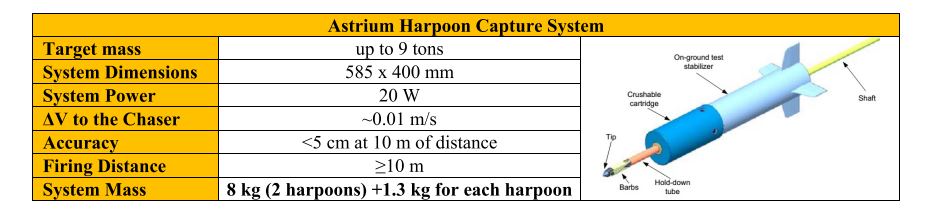
\includegraphics[width=\linewidth]{bilder/Harpune.png}
	\caption{Astrium Harpunen-Systems \citep{ruggiero2015small}} 
	\label{Harpune}
\end{figure}
\noindent Ein mögliches Netz-System wurde am Politecnico di Milano designed und getestet. Es kann je nach dem anvisierten Ziel in unterschiedlicher Größe angefertigt werden. Es besteht aus einem pyramidenförmigen Netz und vier Massen an der Pyramiden-Basis. Diese Massen werden aus der Plattform geschossen. Das Netz ist an der Prymiden-Spitze mit der Plattform über ein Seil verbunden. Durch die Richtung, in die die Massen geschossen wurden, öffnet sich das Netz langsam. Wenn das Ziel das Netz berührt, schließt sich dieses durch die natürliche Dynamik \citep{lavagna2012debris}.
\begin{figure}[H]
	\centering
	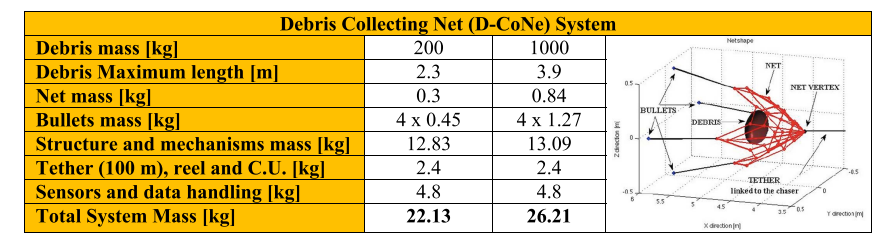
\includegraphics[width=\linewidth]{bilder/Netz.png}
	\caption{Netz-System D-CoNe \citep{ruggiero2015small}} 
	\label{Harpune}
\end{figure}
\noindent Zuletzt ist auch eine \textbf{kontaktlose Verbindung} möglich, z.B. mit einem Ionenstrahl. Dies ist aber für die anvisierten Schrottteile im LEO eher nicht passend.

\subsection{De-orbiting}
Bisher wurde das Verringern der Flughöhe so beschrieben, dass der Satellit das Ziel unter Kontrolle bringt und gemeinsam mit diesem abbremst. Dieses Konzept wird aufgrund des regelmäßigen Aufsteigens und Falls der Plattform "Phoenix" genannt \citep{covello2012application}. Dabei wird das Schrottteil also vom Satelliten auf den Abstell-Orbit transportiert. \\\\
\begin{figure}[H]
	\centering
	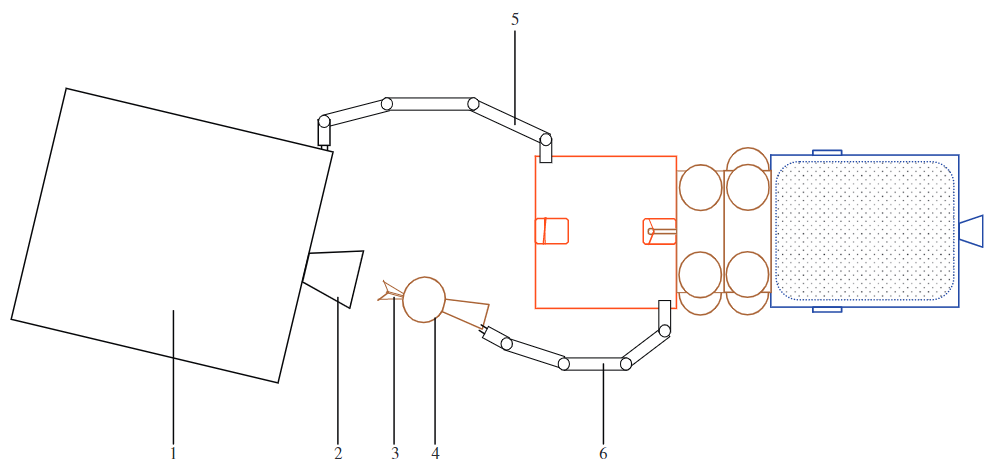
\includegraphics[width=0.8\linewidth]{bilder/Revolver.png}
	\caption{Anbringung einer de-orbitting Vorrichtung \citep{castronuovo2011active}, 1: Müllteil, 2: Düse einer Raketenstufe, 4: De-orbitting Vorrichtung, 5,6: Roboterarme}
	\label{De-orbitting kit}
\end{figure}
\noindent Die Alternative dazu ist "Revolver". Hier wird eine de-orbiting Vorrichtung am Ziel angebracht (siehe \autoref{De-orbitting kit}). Diese feuert, sobald die Verbindung von Plattform und Müllteil wieder getrennt ist und befördert letzteres damit auf den Entsorgungs-Orbit. Diese Methode spart deutlich Treibstoff, da die Plattform sich nach dem de-orbitten nicht wieder nach oben bewegen muss. So könnte sich eine Plattform schnell zwischen vielen Teilen im sonnensynchronen LEO-Orbit bewegen und dabei hauptsächlich den Treibstoff für die de-orbitting Vorrichtungen verbrauchen. Ein Problem bei dieser Methode ist das Anbringen der Vorrichtung am Müllteil, was zum Beispiel durch Schweißen funktionieren soll. Zudem kann hier nicht so einfach der RAAN Drift genutzt werden. \\\\
Aufgrund seiner ressourcen-sparenden Eigenschaften sollte die Revolver-Methode auf lange Sicht eher genutzt werden. Eine weitere Möglichkeit beim Sparen von Kraftstoff ist die Wahl des Antriebs.

\subsection{Antrieb}
Die häufigste Variante, einen Satelliten anzutreiben ist der \textbf{chemische Antrieb}. Dabei wird ein Kraftstoff, z.B. Hydrazin, durch eine chemische Reaktion erhitzt. Das heißes Gas dehnt sich aus und erzeugt so Schub. Der Nachteil dieser Methode ist, dass dabei viel Masse in Form von Kraftstoff und des Tankes mitgeführt werden muss. Ist der Treibstoff aufgebraucht, ist die Plattform nicht mehr steuerbar und die Mission beendet. Dadurch kann nur eine geringe Zahl von Zielen in einer Mission entfernt werden; So müssen viele Missionen durchgeführt werden und die Kosten steigen. \\\\
\textbf{Elektrische Antriebe} benötigen deutlich weniger Kraftstoff. Allerdings können sie auch nicht so viel Schub entwickeln wie chemische Antriebe und benötigen daher deutlich länger, um ein Orbit-Manöver durchzuführen. \\\\
Für elektrische Antriebe gibt es drei verschiedene Konzepte \citep{o2021electric}: beim elektrostatischen Konzept wird Treibstoff ionisiert und durch ein elektrisches Feld beschleunigt. Dazu zählt auch der Hall-Antrieb, der bei Raumfahrzeugen sehr häufig verwendet wird (\autoref{Elektrisch}, zweites Bild von rechts). Bei elktrothermischen Antrieben wird ein Treibstoff in einer Kammer erhitzt und erzeugt beim Austritt aus einer Düse Schub. Bei elktromagnetischen Antrieben wird ebvenfalls ein Treibstoff ionisiert. Hier wird dieser durch das Zusammenspiel von einem elektrischen und magnetischen Feld beschleunigt.
\begin{figure}[H]
	\centering
	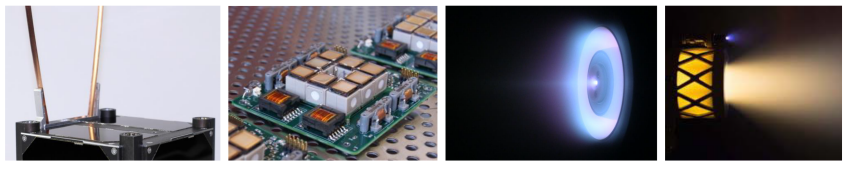
\includegraphics[width=\linewidth]{bilder/ElecP.png}
	\caption{Beispiel von vier verschiedenen elektrostatischen Triebwerken \citep{o2021electric}, die kleinen Dimensionen der Antriebe sind ersichtlich}
	\label{Elektrisch}
\end{figure}
\noindent Eine spezielle Variante des elektromagnetischen Antriebs sind \textbf{elektromagnetische Halteseile} (EDT). Das ist ein langer (mehrere Kilometer), leitender Draht, der zwischen der Plattform und einer Endmasse in radialer Richtung verläuft. Durch die Endmasse wird er unter Spannung gehalten. An beiden Enden des Drahtes befinden sich Plasma-Kontakter Kathoden, die sowohl Elektronen aus dem ionosphärischen Plasma aufnehmen können als auch abgeben. Dadurch fließt ein Strom durch den Draht. Auf die Elektronen wirkt aufgrund des Erdmagnetfeldes eine Lorentz-Kraft. Durch diese wird die Plattform abgebremst oder beschleunigt \citep{levin2012wholesale}.
\begin{figure}[H]
	\centering
	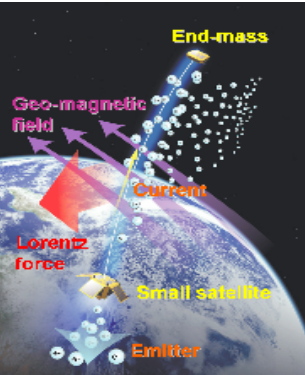
\includegraphics[width=0.5\linewidth]{bilder/EDT.png}
	\caption{Prinzip des elektrodynamischen Halteseils \citep{kobayashi2009deployment}}
	\label{EDT}
\end{figure}
\noindent Die Richtung der Lorentzkraft ist senkrecht zur Geschwindigkeit $\mathbf{v}$ der Elektronen im Draht und dem Erdmagnetfeld $\mathbf{B}$:
\begin{equation} \mathbf{F} = q \mathbf{v} \times \mathbf{B}. \label{Kraft}\end{equation}
Dabei ist $\mathbf{F}$ die wirkende Kraft und $q$ die Ladung eines Elektrons. Die fetten Größen sind als Vektoren zu verstehen. Da an beiden Enden des Drahtes Elektronen aufgenommen und abgegeben werden können, können die Elektronen in beide Richtungen im Draht verlaufen. Die beiden resultierenden Lorentz-Kraft-Vektoren sind einander entgegen gesetzt (siehe \autoref{EDTBoost}). Daher ist einer der Vektoren dem Geschwindigkeits-Vektor der Plattform zumindest zum Teil entgegengesetzt (und einer zeigt zum Teil in seine Richtung), bis auf den Sonderfall, dass beide Vektoren exakt senkrecht zur Bewegungsrichtung sind, was vernachlässigt werde kann. Je nachdem, ob beschleunigt oder gebremst werden will, wird also die Richtung des Stromflusses gewählt.
\begin{figure}[H]
	\centering
	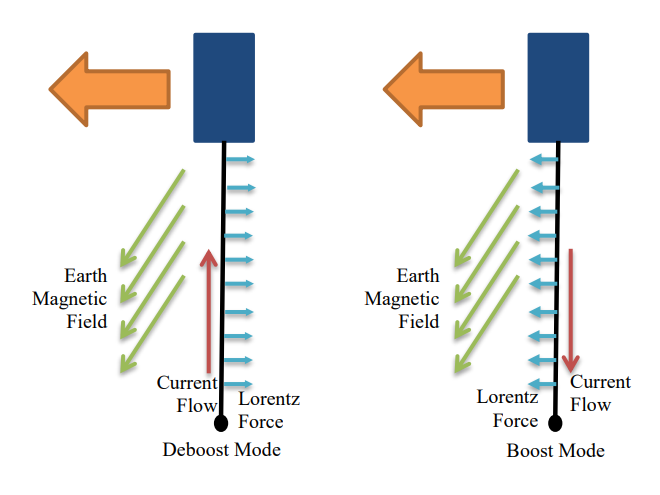
\includegraphics[width=0.6\linewidth]{bilder/EDTBoost.png}
	\caption{Antrieb- und Abbrems-Modus des elektrodynamischen Halteseils \citep{carpenteruse}}
	\label{EDTBoost}
\end{figure}
\noindent Um die Kraft abzuschätzen, die ein solches System erzeugn kann, wird eine Beispielrechnung durchgeführt. Wenn \autoref{Kraft} nur hinsichtlich der Größe betrachtet wird, erhält man $F=Q \cdot v \cdot B_{hor}$. Dabei ist $Q$ die Gesamtladung aller Elektronen, die durch den Draht fließen und $B_{hor}$ der Anteil des Erdmagnetfeld in horizontaler Richtung (da dieser senkrecht zur radialen Richtung des Drahtes ist). Die Geschwindigkeit $v$ der Elektronen im Draht lässt sich umschreiben zu $s/t$ wobei $s$ die Länge des Drahtes und $t$ die Zeit ist, die die Elektronen benötigen, um von einem Ende zum anderen zu gelangen. In dieser Zeit sind exakt alle Elektronen die zum Startzeitpunkt im Draht waren, bis zum Ende gelaufen. Das bedeutet, das $t$ ist dasselbe, das in der Formel der Stromstärke $I=Q/t$ vorkommt. Damit lässt sich \autoref{Kraft} umschreiben und man kann mit typischen Werten für die einzelnen Größen eine Kraft schätzen:
\begin{equation} F = Q \cdot v \cdot B_{hor} = Q \cdot s/t \cdot B_{hor} = Q/t \cdot s \cdot B_{hor} = I \cdot s \cdot B_{hor} = 1 A \cdot 10 km \cdot 20 \mu T = 0.2 N. \end{equation} 
Hier wurde von einem 10 km langen Halteseil, einer Stromstärke von 1 A und einer Stärke des Magnetfelds in horizontaler Richtung von 20 $\mu$T ausgegangen. Das Ergebnis ist ein Wert für die resultierende Kraft. Diese zeigt allerdings nicht genau in Bewegungsrichtung, das heißt die Aswirkung auf die Geschwindigkeit wird tatsächlich mit einer geringeren Kraft stattfinden. Bei diesem Konzept treten immer cross-track-Kräfte auf, die die Inklination und Rektaszension der Plattform verändern und beim Manövrieren berücksichtigt werden müssen \citep{carpenteruse}. \\
Durch die Nutzung des Erdmagnetfeldes benötigt dieser Antrieb keinen Treibstoff. Die elektrische Leistung für die Kathoden kann durch Solarzellen gewonnen werden. Damit sind sehr lange Missionen denkbar. Allerdings sind die erreichten Leistungen, wie die Rechnung gezeigt hat, weit entfernt von denen anderer Antriebe. Es wird also kein kurzer starker Schub ausgeführt, der die Plattform auf einen elliptischen Transfer-Orbit (Hohmann-Transfer) bringt, sondern es wird eine konstante Kraft über eine lange Zeit übertragen. Damit ist dieses Verfahren zeitintensiver. Ein einzelner de-orbit Vorgang kann Wochen bis Monate dauern. Außerdem ist die große Formation schwieriger zu manövrieren und die Wahrscheinlichkeit, von einem anderen Partikel getroffen zu werden, steigt. Das EDT-Verfahren ist noch weniger erprobt als klassische Antriebe, dürfte aber aufgrund der genannten Vorteile in Zukunft eine wichtige Rolle spielen.

\subsection{Warenhaus}
Eine andere Idee, um die Missionsdauer zu verlängern, ist das Warenhaus-Konzept \citep{castronuovo2011active}. Dies ist ein Satellit, der Treibstoff für die Plattform, sowie eventuell de-orbiting Vorrichtungen geladen hat. Diese tauscht er mit der Plattform aus. \\\\
Das Warenhaus wird in den Orbit der Plattform geschickt. Es wird ein Rendez-vous und ein Andocken mittels Roboterarmen durchgeführt. Durch einen modularen Aufbau der Plattform und des Warenhauses, müssen nur einzelne Module an- und abgekoppelt werden (siehe \autoref{Warenhaus}). Die Fracht- (de-orbiting Geräte) und Treibstoff-Module werden ausgetauscht und das Warenhaus de-orbited sich wieder.\\\\
Durch das Warenhaus kann Budget gespart werden, da es nicht alle Bestandteile der Plattform mitführen muss. Die Software und Kameras für das rendez-vous sind ebenso nicht nötig wie die Verbindungs-Vorrichtung (Roboteram). Allerdings wird weiterhin ein zusätzlicher Raketenstart für das Warenhaus benötigt, sodass die Nutzen des Konzepts begrenzt sind.
\begin{figure}[H]
	\centering
	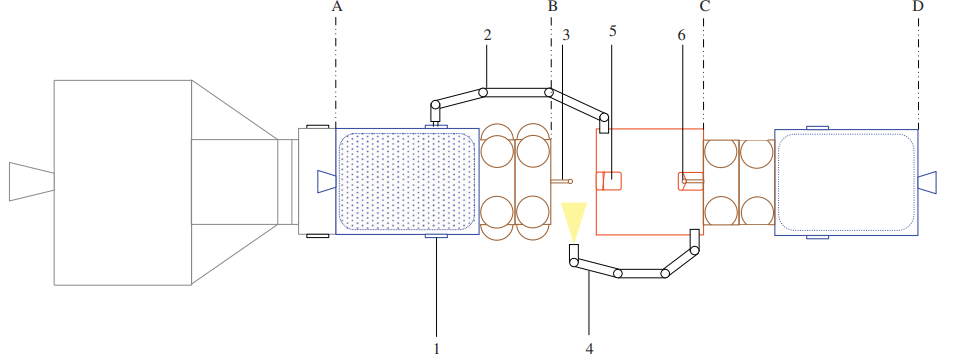
\includegraphics[width=\linewidth]{bilder/Warenhaus.png}
	\caption{Darstellung des Nachschub-Vorgangs \citep{castronuovo2011active}, links ist das Warenhaus mit den neuen de-orbit Geräten (braun) und Treibstoff (blau) zu sehen, rechts die Plattform}
	\label{Warenhaus}
\end{figure}

\subsection{Aktueller Stand} \label{aktuell}
Bislang ist keine Raumschrott-Entsorgungs-Mission bekannt, die in Operation ist. \\\\
Im Januar 2022 wurde allerdings von einer amerikanischen Weltraumüberwachungs-Firma beobachtet, wie der chinesischer GEO-Satellit SJ-21 ein rendez-vous mit dem nicht mehr funktionsfähigen Satelliten Compass-G2 ausführte. Die beiden Satelliten blieben für vier Tage verbunden, bis G2 auf einem Abstell-Orbit 3000 km über GEO freigelassen wurde \href{https://www.dw.com/en/chinese-space-cleaner-spotted-grabbing-and-throwing-away-old-satellite/a-60658574}{(https://www.dw.com/en/chinese-space-cleaner-spotted-grabbing-and-throwing-away-old-satellite/a-60658574)}. Danach kehrte SJ-21 auf seinen ursprünglichen Orbit zurück. Details über den Vorgang und weitere Pläne sind aufgrund der chinesischen Geheimhaltung aber nicht bekannt. \\\\
Die japanische Firma Astroscale führte 2021-2022 die Mission ELSA-d (Demostration) durch, bei der das Auffinden und Einfangen eines Müllteils gezeigt werden sollte. Dazu wurde eine Plattform zusammen mit einem Klient in den LEO-Orbit geschossen. Die Plattform sollte den Klient mehrmals freigeben und wieder ergreifen. Eine Test-Ergreifung im August 2021 war erfolgreich. Dabei entfernte sich der Klient nur wenige Zentimeter und wurde dann mit einem magnetischen Mechanismus wieder eingefangen. Die nächste Missionphase, in der sich der Klient weiter weg bewegen sollte vor dem Wiedereinfangen, konnte nach Problemen mit mehreren Triebwerken nicht erfolgreich abgeschlossen werden. Allerdings wurde ein far-range rendezvous mit absoluter Navigation bis auf eine Entfernung von 160 m durchgeführt und auch die Übergabe von absoluter zu relativer Navigation ergab ein positives Ergebnis. (\href{https://www.eoportal.org/satellite-missions/elsa-d#mission-status}{https://www.eoportal.org/satellite-missions/elsa-d})
\begin{figure}[H]
	\centering
	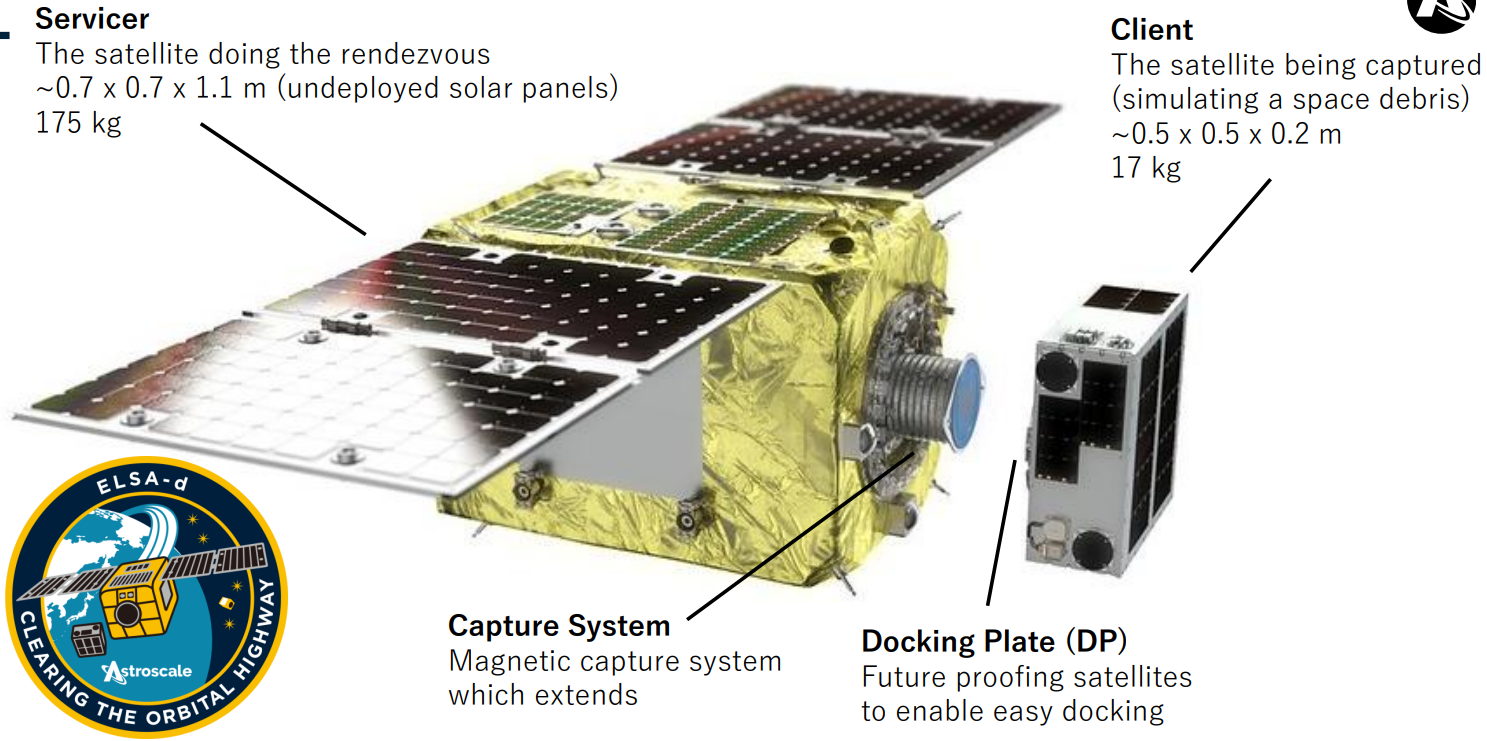
\includegraphics[width=\linewidth]{bilder/ELSAd.png}
	\caption{Darstellung von Plattform und Klient der ELSA-d Mission \url{https://indico.esa.int/event/321/contributions/6383/attachments/4369/6591/ESA\%2520CleanSpace\%25202021\%2520-\%2520Astroscale\%2520ELSA-d.pdf}}
	\label{ELSAd}
\end{figure}
\noindent Ein richtiges Schrottteil soll die Clearspace-1 Mission der ESA entfernen. Ihr Ziel ist eine Raketenstufe im LEO mit einer Masse von 112 kg. Die Mission wurde 2019 auf den Weg gebracht und befindet sich aktuell in der Design-Phase. Der Start ist nach einer Verschiebung nun für 2026 geplant. Die Plattform wird eine Masse von 500 kg haben und besitzt einen klassischen chemischen Antrieb mit Hydrazin. Zur Navigation sind visuelle Kameras sowie Radar- und Laser-Systeme an Bord. Das Ziel soll mit vier Tentakeln ergriffen und gesichert werden (siehe \autoref{capture}). Die Plattform und die Raketenstufe sollen gemeinsam de-orbiten und in der Atmosphäre verglühen. Das Missionsbudget von etwa 120 Millionen Schweizer Franken (Stand 2021) zeigt eines der Hauptprobleme, warum die Raumschrottentsorgung noch so wenig weit fortgeschritten sind: angesichts der großen Zahl der Teile ist das Entsorgen eines einzelnen Ziels schon extrem teuer.
\begin{figure}[H]
	\centering
	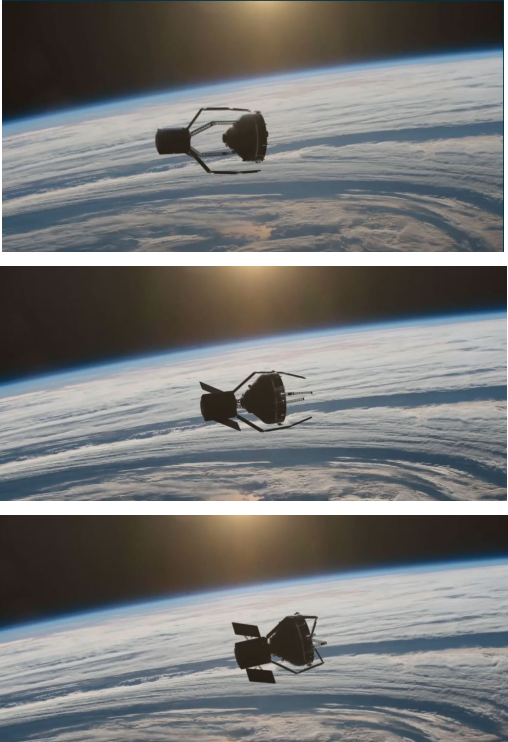
\includegraphics[width=0.55\linewidth]{bilder/ClearspaceCapture.png}
	\caption{Künstlerische Darstellung des Einfangens bei der Clearspace-1 Mission \citep{biesbroek2021clearspace}}
	\label{capture}
\end{figure}
\noindent Eine andere Herausforderung ist die technische Seite. Vor allem der Umgang mit taumelnden Objekten ist bislang wenig erprobt. Bei bislang durchgeführten Remdez-vous, zum Beispiel mit der Internationalen Raumstation, handelt es meist um stabile Objekte. Bei einem taumelnden Teil kann es passieren, dass bei einem gescheiterten Andocken die Plattform zerstört wird und neue Wolken von Müll entstehen. \\\\
Weiterhin gibt es legale Probleme bezüglich des Besitzes eines Weltraumobjekts. Auch wenn es nicht mehr in Betrieb ist, gehört es rechtlich der Organisation, die es betrieben hat. Deshalb hat die Clearspace-1 Mission auch eine Raketenstufe eines früheren ESA-Starts zum Ziel. \\\\
Das Budget von Clearspace-1 macht ersichtlich, was für Summen aufgewendet werden müssen, um einen wirklichen Effekt auf die Situation zu haben. Offensichtlich wird das Problem noch nicht als ernst genug gesehen, damit die verschiedenen Weltraumbehörden mit Nachdruck Raumschrott-Ensorgungs-Missionen auf den Weg bringen. \\\\
Die weiter oben beschriebenen Entwicklungen der letzten Jahre zeigen aber, dass sich diese Situation wandelt und in den nächsten Jahrzehnten häufige Missionen üblich werden sollten.

\subsection{Rendez-vous Simulation} \label{rendez-vous}
Eine der schwierigsten Phasen einer satelliten-basierten Müllentsorgungs-Mission ist das Rendez-vous. Neben den Herausforderungen, das Zielobjekt mit den relativen Navigationssensoren zu erfassen, sich an die Rotation anzupassen und das Teil zu greifen und zu sichern, muss auch die Orbitmechanik zwischen den beiden Objekten verstanden werden. \\\\
Mit einer Matlab-Simulation wird der Ablauf des Phasings und des rendez-vous untersucht. Als Grundlage dienen die Lösungen der homogenen Hill-Gleichungen:
\begin{figure}[H]
	\centering
	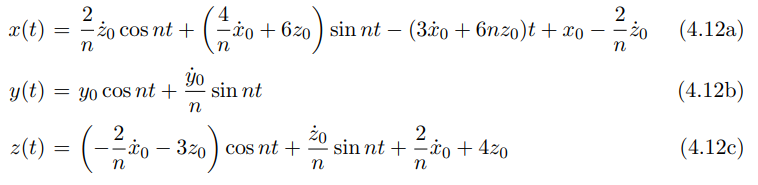
\includegraphics[width=\linewidth]{bilder/Hill.png}
	\caption{homogene Lösung der Hill-Gleichungen}
	\label{Hill}
\end{figure}
\noindent Die Gleichungen beschreiben die Bewegung eines anderen Körpers (der Plattform) bezüglich eines Satelliten (dem Zielteil) im Hill-frame. Dieses hat seinen Ursprung im Satelliten; die x-Achse zeigt in die Bewegungsrichtung des Satelliten, die y-Achse zeigt across-track und z radial. Die Hill-Gleichungen erhält man, wenn man die Orbitdynamik bezüglich eines radialen Gravitationsfeldes betrachtet. Störkräfte wie die Erdabplattung sind nicht berücksichtigt. \\\\
Die Lösung beschreibt, wie sich die Plattform bei bestimmten Anfangsbedingungen, nämlich der relativen Position und Geschwindigkeit zum Zielobjekt, über die Zeit verhält. Der Ablauf der Simulation ist: die Gleichungen wurden nach $t$ abgeleitet, um zusätzlich die aktuelle Geschwindigkeit zu berechnen. Mit diesen Gleichungen wird sekündlich die Position und Geschwindigkeit der Plattform im Hill-frame berechnet. Zu bestimmten Zeitpunkten wird auf den berchneten Wert der Geschwindigkeit in along-track Richtung ($\dot{x}$) ein Wert addiert. Durch einer Reihe solcher x-Schübe wird die Position und Geschwindigkeit nach und nach an die des Zielobjekts angepasst. Die y-Komponente wurde hier nicht beachtet, da sie von $x$ und $z$ entkoppelt ist. \\\\
Als Orbit-Höhe wurde 800 km gewählt. Die Plattform startet 200 km hinter dem Ziel ($x_0$) und 2 km darunter ($z_0$), während die relative Geschwindigkeiten 0 sind. Wenn kein Schub angebracht wird, sieht man, dass die Plattform das Ziel innerhalb kurzer Zeit überholt. Es ist zu sehen, dass sich die Plattform automatisch in einem Bogen-Verlauf bewegt, wie er in \autoref{Rendezvous} zu sehen war. Ein Bogen entspricht dabei einem Orbitumlauf, der auf dieser Höhe etwa 100 Minuten dauert.
\begin{figure}[H]
	\centering
	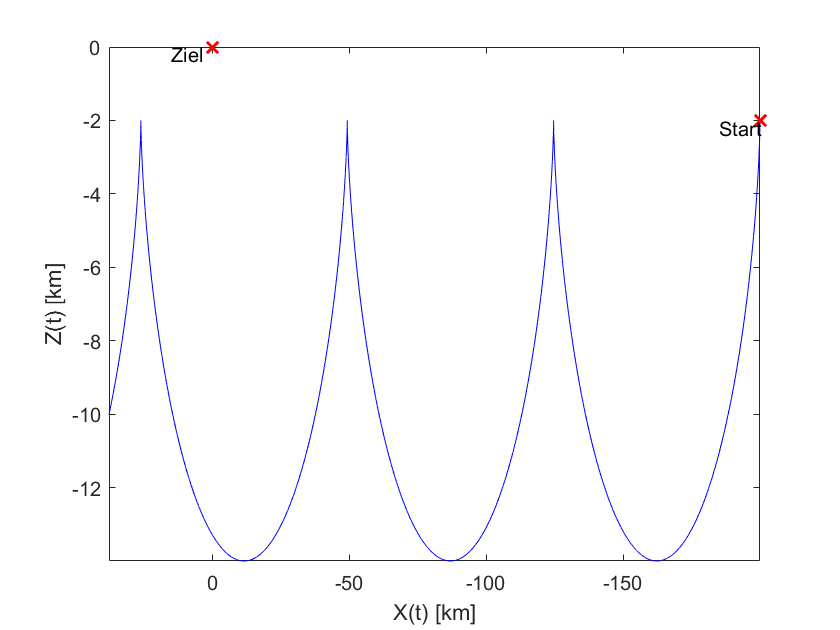
\includegraphics[width=0.6\linewidth]{bilder/Phasing.png}
	\caption{Rendez-vous Simulation ohne Schübe, x-Achse ist gespiegelt. Flugrichtung des Zielsatelliten ist nach links, die Plattform startet von der rechten Seite}
	\label{Phasing}
\end{figure}
\noindent Da die Plattform im dritten Orbit das Ziel überholt, wird am Ende des zweiten Orbits ein x-Schub angebracht mit $\Delta v = 2.5 m/s$. Dadurch wird der Bogen verkleinert und die Relativgeschwindigkeit zum Ziel verringert sich. Dieses Vorgehen wird mehrmals wiederholt, bis sich Position und Geschwindigkeit kaum noch unterscheiden.
\begin{figure}[H]
	\centering
	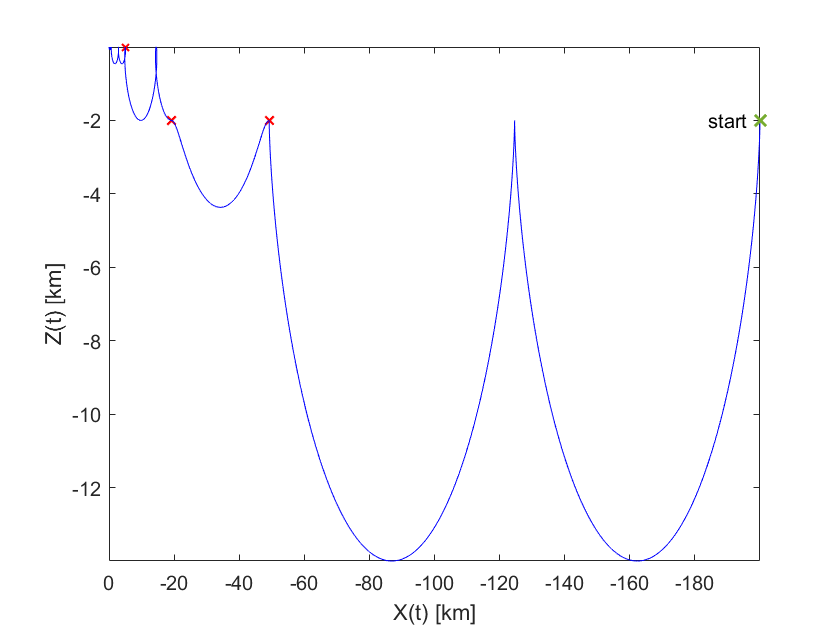
\includegraphics[width=0.6\linewidth]{bilder/RendezvousPhase1A.png}
	\caption{Rendez-vous Simulation mit x-Schüben, 1. Phase (Phasing), die roten Kreuze makieren die Orte der Schübe}
	\label{Phasing}
\end{figure}
\noindent Nach drei Schüben und 5 Kilometer hinter dem Ziel wird vom Phasing zum far-range rendez-vous übergegangen. Technische Aspekte wie absolute und relative Navigation kann hier alleridngs nicht beleuchtet werden.
\begin{figure}[H]
	\centering
	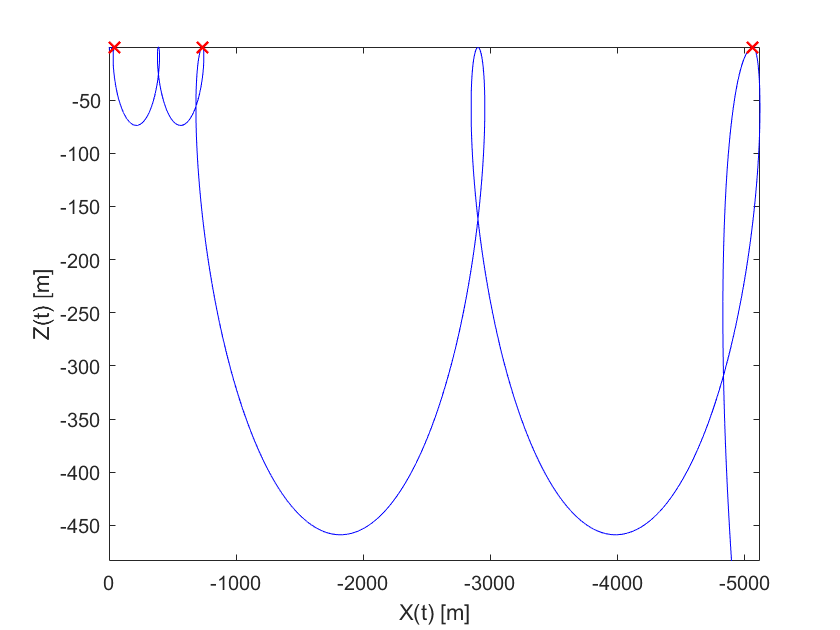
\includegraphics[width=0.6\linewidth]{bilder/RendezvousPhase2A.png}
	\caption{Rendez-vous Simulation mit x-Schüben, 2. Phase (far-range rendez-vous)}
	\label{frrendez}
\end{figure}
\noindent Nach zwei weiteren Schüben ist die Plattform nur noch einige Meter von ihrem Ziel entfernt. Dann kann mit dem close-range Rendezvous begonnen werden, wobei Nahfeldkameras und Nahfeldlaser zum Einsatz kommen. Nach dem 6. Schub weißt die Plattform fast keine Relativgeschwindigkeit zum Ziel mehr auf. Innerhalb eines Bogens (einem Zeitfenster von 100 Minuten) bewegt es sich nur wenige Zentimeter. Nun könnte ein fly-around oder ein Andocken beginnen.
\begin{figure}[H]
	\centering
	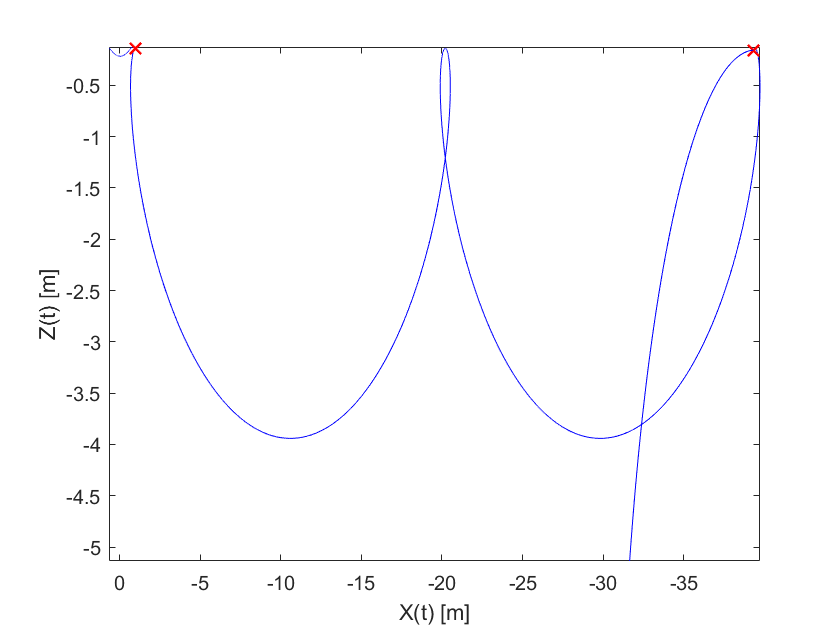
\includegraphics[width=0.6\linewidth]{bilder/RendezvousPhase3A.png}
	\caption{Rendez-vous Simulation mit x-Schüben, 3. Phase (close-range rendez-vous)}
	\label{crrendez}
\end{figure}

\clearpage
\section{Laserbasierte Methoden}\label{sec:laser}
Das Eliminieren von Weltraumschrott, wie es bislang im Rahmen der mechanischen Verfahren vorgestellt wurde, beschränkt sich nahezu vollständig auf Objekte größer als \SI{10}{\centi\meter}. Für kleinere Objekte währe ein entsprechendes Verfahren jedoch sehr ineffizient und teilweiße schlicht nicht durchführbar. Aus diesem Grund, und aufgrund einer proklamierten höheren Effizienz, stellen laserbasierte Systeme, welche auch kleinere Objekte zum Absturz bringen können, eine vielversprechende Lösung dar.\\\\
Die Entfernung von Weltraumschrott im LEO-Bereich mittels Laser, wie sie im folgenden vorgestellt wird, basiert grundlegend auf dem Konzept der Impulsübertragung durch Laser-Ablation. 
\begin{figure}[H]
	\centering
	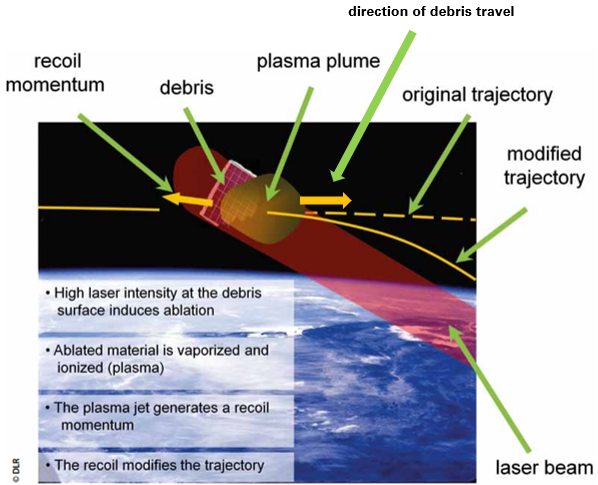
\includegraphics[width = 0.9\textwidth]{images/ablation mod.png}
	\caption{Laser Ablation nach \citet{eckel2016laser}}
	\label{ablschema}
\end{figure}
\noindent
Ein energetisch hochgenau dosierter Laserimpuls wird in Richtung des Schrottteilchens emittiert, auf dessen Oberfläche hierdurch der Ablationsvorgang beginnt. Das durch diesen abgetragene Material erzeugt anschließend eine Plasma-Wolke in Flugrichtung sowie einen entgegengesetzt wirkenden Rückstoß. Dieser verlangsamt das Objekt und sorgt somit für eine Änderung der Flugbahn. Durch wiederholten Beschuss kann hierdurch eine Geschwindigkeitsreduktion erreicht werden, die die Perigäumshöhe des Teilchens ausreichend reduziert, um dieses schließlich in der Atmosphäre verglühen zu lassen. Während des Beschusses muss dabei stets gewährleistet sein, dass das Schrottteilchen durch den Laser nicht zerstört und in kleinere Teilchen zersprengt wird. Dies bedingt im Umkehrschluss eine benötigte hohe Energieeffizienz und Anpassungsfähigkeit des Lasers, die einen hochfrequenten Beschuss mit einer angepassten Energiemenge pro Schuss erlaubt.\\\\
Während ein solches Verfahren in der Vergangenheit aufgrund von Einschränkungen wie der Größe von Lasern oder deren schlechter Energieeffizienz lediglich auf dem Boden denkbar war \citep{p12q6lreq}, so ermöglichen Innovationen in der Lasertechnik, wie zum Beispiel der ICAN Laser \citep{icanlaser}, seit einigen Jahren die Entwicklung von satellitengestützten Systemen. 

\subsection{Laser Orbital Debris Removal (LODR)}
Laser Orbital Debris Removal (LODR) ist ein bodengestütztes Laser-System zur Eliminierung von Weltraumschrott, welches 1996 von \citet{phipps1996orion} vorgeschlagen und auf Basis von technologischen Fortschritten 2012 weiter optimiert wurde \citep{phipps11}. 
\begin{figure}[H]
	\centering
	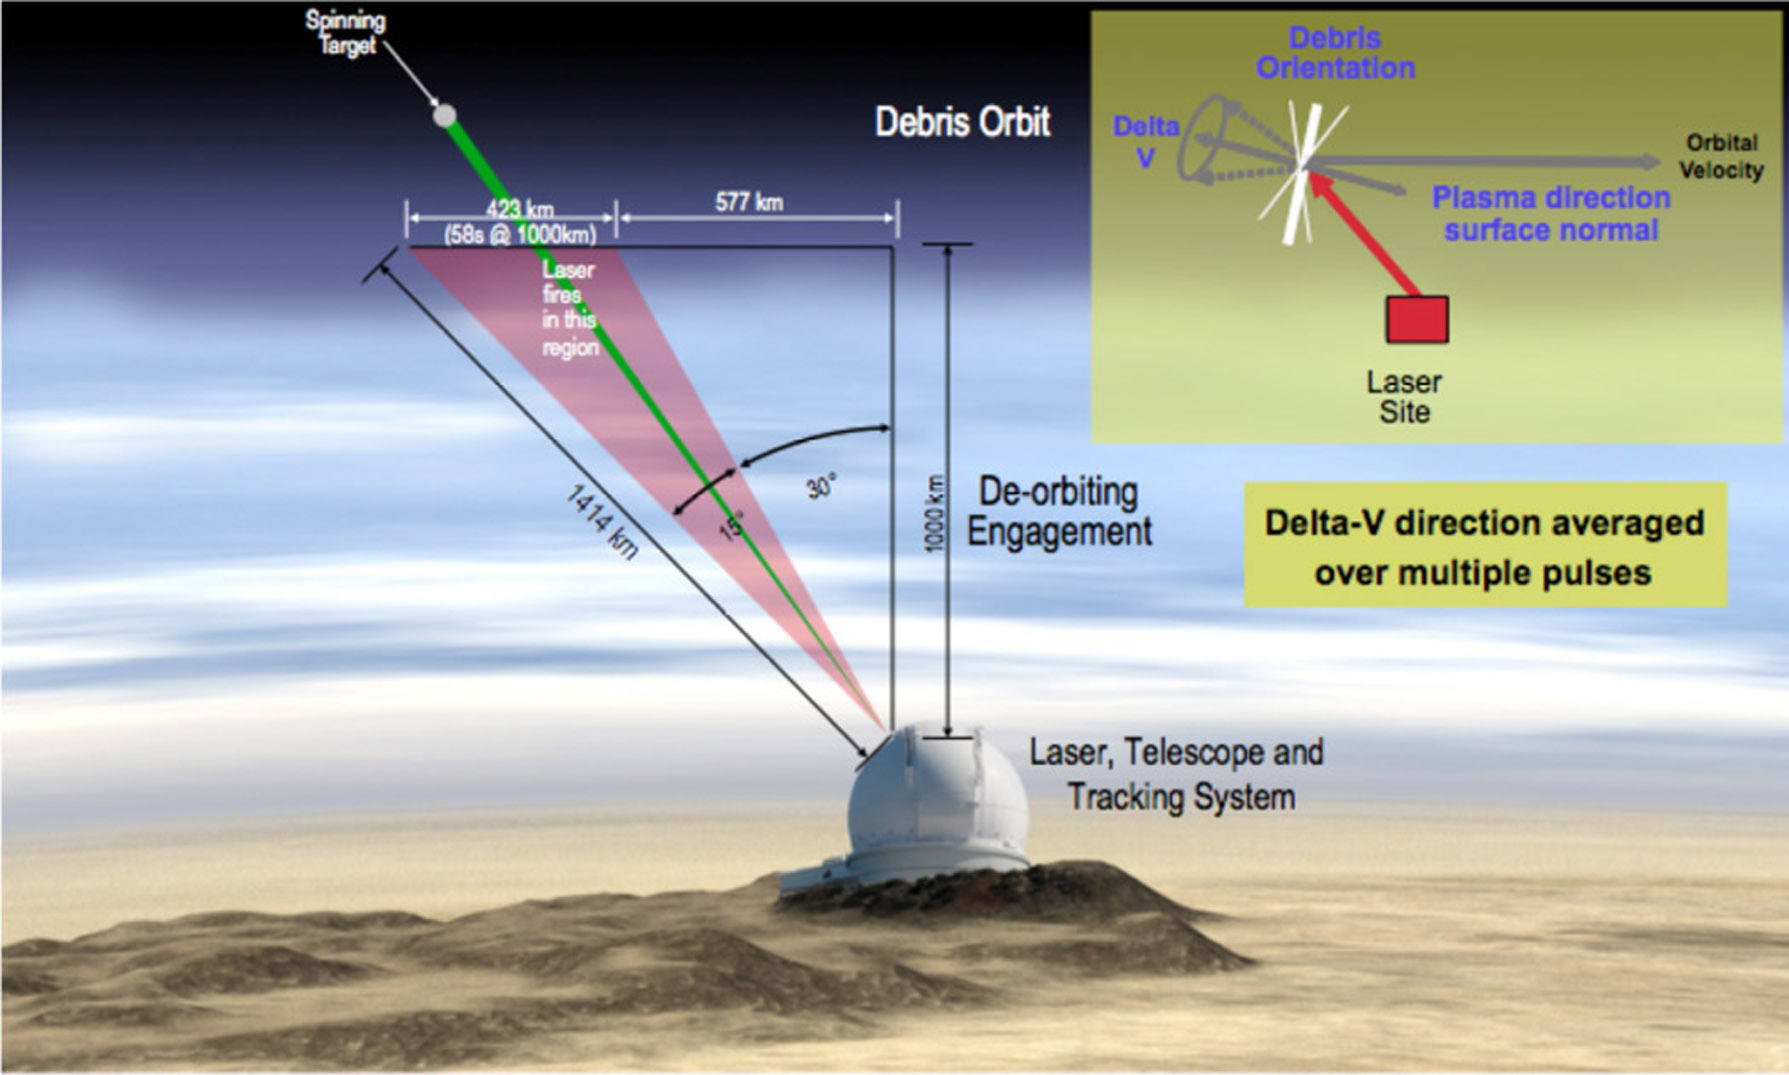
\includegraphics[width = 0.9\textwidth]{images/LODR_konzept.jpg}
	\caption{LODR Schema nach \citet{phipps11}}
	\label{lodrschema}
\end{figure}
\noindent \autoref{lodrschema} zeigt den schematischen Aufbau von LODR. Ein Laser wird von der Bodenstation aus wiederholt auf ein Objekt im Überflug geschossen. Dessen Orbit muss hierfür bekannt sein, damit der Laser zum Zeitpunkt an dem er die Objekthöhe erreicht hat, auch sein Ziel trifft (look-ahead). Eine hohe Genauigkeitsanforderung muss außerdem an die Teleskope bzw. die komplette Abschussmechanik gestellt werden, um den Sateliten zuverlässig zu treffen. Die Richtung des in \autoref{ablschema} gezeigten Rückstoßes, in \autoref{lodrschema} durch \textit{Delta-V} gekennzeichnet, ergibt sich dabei aus der Summe aller abgegebenen Schüsse. Damit die Objektlaufbahn im gewünschten Maß verändert wird, \textit{Delta-V} also in die richtige Richtung zeigt, werden Schüsse nur in einem Zenitwinkel zwischen \SI{45}{\degree} und \SI{30}{\degree} abgegeben.\\\\
Angenommen der Laser bewegt sich mit einem Zenitwinkel von \SI{45}{\degree} durch die Atmosphäre bis zu einem Objekt mit Orbit Höhe $A_o = $\SI{1000}{\kilo\meter}, so ergibt sich zunächst eine Distanz von \SI{1414}{\kilo\meter} und damit eine Laufzeit von \SI{4.7}{\milli \meter}. Die Geschwindigkeit des Objektes im Orbit ergibt sich mit 
\begin{equation}
	\label{objspeed}
	v_o=\sqrt{\frac{GM_E}{r}}=\sqrt{\frac{GM_E}{R_E+A_o}}
\end{equation}
\noindent
wiederum zu \SI{7346.436}{\meter \per \second}.
Die während der Laufzeit zurückgelegte Strecke des Objektes ergibt sich somit zu circa \SI{34.528}{\meter}, was einer Bewegung der Abschussmechanik um  \SI{2.44e-5}{\radian} entspricht. Diese muss sich somit mit einer Winkel- geschwindigkeit von \SI{7.35}{\milli \radian \per \second} mitdrehen, um die Objektbewegung im Laufe wiederholter Schüsse zu kompensieren. Im Falle eines Objektdurchmessers von \SI{10}{\centi \meter} sowie eines Laserdurchmessers von \SI{30}{\centi \meter} ist zusätzlich eine Genauigkeit des Abschusswinkels von $\pm$ \SI{7.01e-8}{\radian} notwendig.\\\\
LODR ist bedeutend günstiger umzusetzen als eine satellitenbasierte Lösung und erlaubt es, abhängig von der Schusszahl, nahezu beliebig große Objekte zu bearbeiten. Zusätzlich ist die Lebensdauer quasi unbegrenzt, solange eine regelmäßige Wartung durchgeführt wird. Des Weiteren können mehrere Objekte quasi parallel verlangsamt werden, da keine Orbitanpassung zwischen zwei Objekten benötigt wird, wie es zum Beispiel beim Collective-Prinzip der Fall ist. Problematisch ist jedoch die schwierige Zielfindung sowie das Tracking einzelner Objekte, welches gerade für den Look-Ahead unabdingbar ist. Dieses ist zwar theoretisch möglich (zum Beispiel mit Hilfe eines Pusher Lasers \citep{phipps1996orion}), benötigt jedoch große Mengen an Energie und ist nur bedingt praktikabel für kleine Objekte. Zudem bedingt das Arbeiten vom Erdboden aus, dass der Laser die Atmosphäre durchdringen muss. Einer der Haupteffekte der hierbei auftrifft, ist die Atmosphären-Szintillation. \citet{phipps1996orion} schlägt hier die Verwendung von adaptiven Optiken \citep{adptoptics} vor, einem Spiegelsystem, welches in der Lage ist, entsprechende Effekte zu kompensieren. 

\subsubsection{Laser und Genauigkeit}
Ein Gelingen von obigem Konzept ist maßgeblich von der Wahl des Lasers abhängig. Wichtige Parameter hierbei sind unter anderem: Wellenlänge, Laserdurchmesser am Ziel und Pulsenergie (Eine genauere Vorstellung der Parameter wird an dieser Stelle nicht vorgenommen, da Sie den Umfang dieser Arbeit überschreiten würde. Grundlegend kann jedoch gesagt werden, dass der Laser entsprechend der benötigten Anforderungen zur Objektverlangsamung konzipiert werden muss. Diese kann auf Basis des Hohmann Ansatzes nach \citet{liedahl2013pulsed} bestimmt werden. 
\begin{figure}[H]
	\centering
	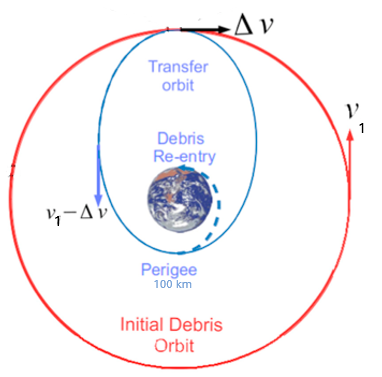
\includegraphics[width = 0.7\textwidth]{images/hohman mod.png}
	\caption{Hohmann Ansatz nach \citet{soulard2014ican} (modifiziert)}
	\label{htschema}
\end{figure}
\noindent
Im Falle einer ausgehenden Kreisbahn mit Radius $R_E+h_A$, wobei $R_E$ dem Erdradius und $h_A$ der Apogäumshöhe entspricht, ist die Geschwindigkeit eines Objektes zunächst gegeben durch
\begin{equation}
	\label{kbspeed}
	v_1^2=\frac{G M}{R_E+h_A}.
\end{equation}
\noindent
Auf Basis der Vis-Viva-Gleichung ergibt sich des Weiteren die Geschwindigkeit auf einer elliptischen Bahn (Transfer Orbit) zu
\begin{equation}
	\label{zweispeed}
	v_2^2=\frac{2 G M}{R_E+h_A}-\frac{G M}{2R_E+h_A+h_p},
\end{equation}
\noindent
wobei $h_p$ der Perigäumshöhe der elliptischen Bahn entspricht. Um ein Objekt von der Kreisbahn auf die elliptische Bahn zu transferieren wird ein Geschwindigkeitsunterschied von $\Delta v = v_2 - v_1$ benötigt, dementsprechend folgt mit Hilfe von $GM=v_1^2\cdot (R_E+h_A)$:
\begin{equation}
	\label{deltaspeed}
	\Delta v = \sqrt{v_1^2-\frac{2GM}{2R_E+h_A+h_p}}-v_1,\mathrm{\ bzw.\ } \frac{\Delta v}{v_1} = \sqrt{\frac{2(R_E+h_p)}{2R_E+h_A+h_p}}-1.
\end{equation}
\noindent
Unter der Annahme einer ursprünglichen Apogäumshöhe $h_A=$ \SI{1000}{\kilo\meter} und einer Perigäumshöhe von $h_p=$ \SI{100}{\kilo \meter}, welche für den Wiedereintritt des Objektes ausreicht, ergibt sich somit $\frac{\Delta v}{v_1} \approx \SI{3.3}{\percent}$ bzw. eine benötigte Geschwindigkeitsreduktion um $v_o\cdot \SI{3.3}{\percent}\approx$ \SI{242.43}{\meter \per\second}.
\\\\
Die Anzahl der benötigten Schüsse, um die Geschwindigkeitsreduktion zu erreichen, kann im Anschluss in Abhängigkeit von verschiedenen Parametern der Laserinteraktion mit dem zu verlangsamenden Objekt sowie der Atmosphäre bestimmt werden. Phipps et Al.\cite{p11q3orion} nennt hier beispielhaft ein Ergebnis von 75 benötigten Schüssen für ein Objekt in \SI{1000}{\kilo\meter} Höhe (am Apogäum) mit Durchmes- ser \SI{5}{\centi\meter} und Gewicht \SI{10}{\gram}. Unter Annahme einer Laser-Schussrate von \SI{0.5}{\hertz} würden also \SI{37.5}{\second} benötigt, um das Objekt in den benötigten Transferorbit zu verschieben. Dies ist innerhalb des, aufgrund der Optimierung der Impulsübertragung von \citet{phipps11} empfohlenen, Schuss-Bereichs im Zenitwinkel von \SI{45}{\degree} und \SI{30}{\degree} problemlos möglich, da das Objekt für die insgesamt knapp \SI{422}{\kilo\meter} unter Annahme einer Geschwindigkeit von \SI{7346.436}{\meter \per \second} ungefähr \SI{57.5}{\second} benötigt.\\\\
Während im Rahmen dieses Berichts die Berechnungen unter der Annahme einer einflussfreien Umgebung durchgeführt wurden, so müssen in der Realität verschiedene zusätzliche Einflüsse beachtet werden, deren Ursprung vor allem in der Atmosphäre zu finden ist. Ein Beispiel hierfür wäre die Atmosphärenszintillation, welche die Laufbahn des Lasers selbst verändert. Um entsprechende Einflüsse zu verringern, teils sogar nahezu vollständig zu entfernen, gibt es verschiedene Ansätze. So können beispielsweise die Wellenlänge und andere Lasereigenschaften verändert werden, um ein möglichst verlustfreies Durchdringen der Atmosphäre zu gewährleisten. Auch der Einfluss atmosphärischer Szintillationseffekte kann durch Verwendung von adaptiven Optiken, einem variablen Spiegelsystem, verringert, bzw. nahezu vollständig kompensiert werden. Vorraussetzung hierfür ist jedoch ein ausreichendes Wissen über die entstehende Ablenkung.

\subsubsection{Tracking und Identifizierung}
Der Abschuss eines Objekts mit dem oben beschriebenen System bedingt ein adäquates Wissen über Objektbewegung und somit Orbiteigenschaften, um in Anbetracht der hohen Genauigkeitsanforderungen einen erfolgreichen Beschuss zu gewährleisten. Hierfür wird ein Tracking- und Identifizierungsverfahren benötigt, welches in der Lage ist, diese Informationen schnell und genau für Objektgrößen von bis zu \SI{1}{\centi\meter} bereitzustellen. \citet{phipps1996orion} schlägt hierfür die Verwendung eines sogenannten Pusher Lasers vor, welcher durch aktive Beleuchtung des Himmels in Kombination mit einer Empfangsoptik in der Lage ist, Objekte mit hohem Albedo bis \SI{1.5}{\centi\meter} in \SI{1500}{\kilo\meter} Höhe zu detektieren und dabei den gesamten Himmel innerhalb von 2 Jahren abzusuchen. Ein großer Vorteil des Systems im Zusammenhang mit LODR besteht darin, das das eingebaute Spiegelsystem als Empfangoptik für den Pusher Laser verwendet kann, wodurch ein zusätzlicher Spiegel obsolet wird. Nachteilhaft ist jedoch der große Energieverbrauch des Lasers, welcher eine Durchschnittsleistung von \SI{30}{\kilo\watt} benötigt, gepaart mit einer geringeren Genauigkeit als vergleichbare Satellitensysteme wie dem ICAN Based Orbital Solar-Powered Debris Sweeper.

\subsection{ICAN Based Orbital Solar-Powered Debris Sweeper}
ICAN Based Orbital Solar-Powered Debris Sweeper (ICAN Sweeper) ist ein satellitengestütztes Laser-System zur Erkennung, Katalogisierung und Entfernung von Weltraumschrott, welches 2014 von \citet{soulard2014ican} vorgestellt wurde und auf Basis des hocheffizienten Glasfaser-Lasersystems ICAN (International Coherent Amplification Network) basiert. 
\begin{figure}[H]
	\centering	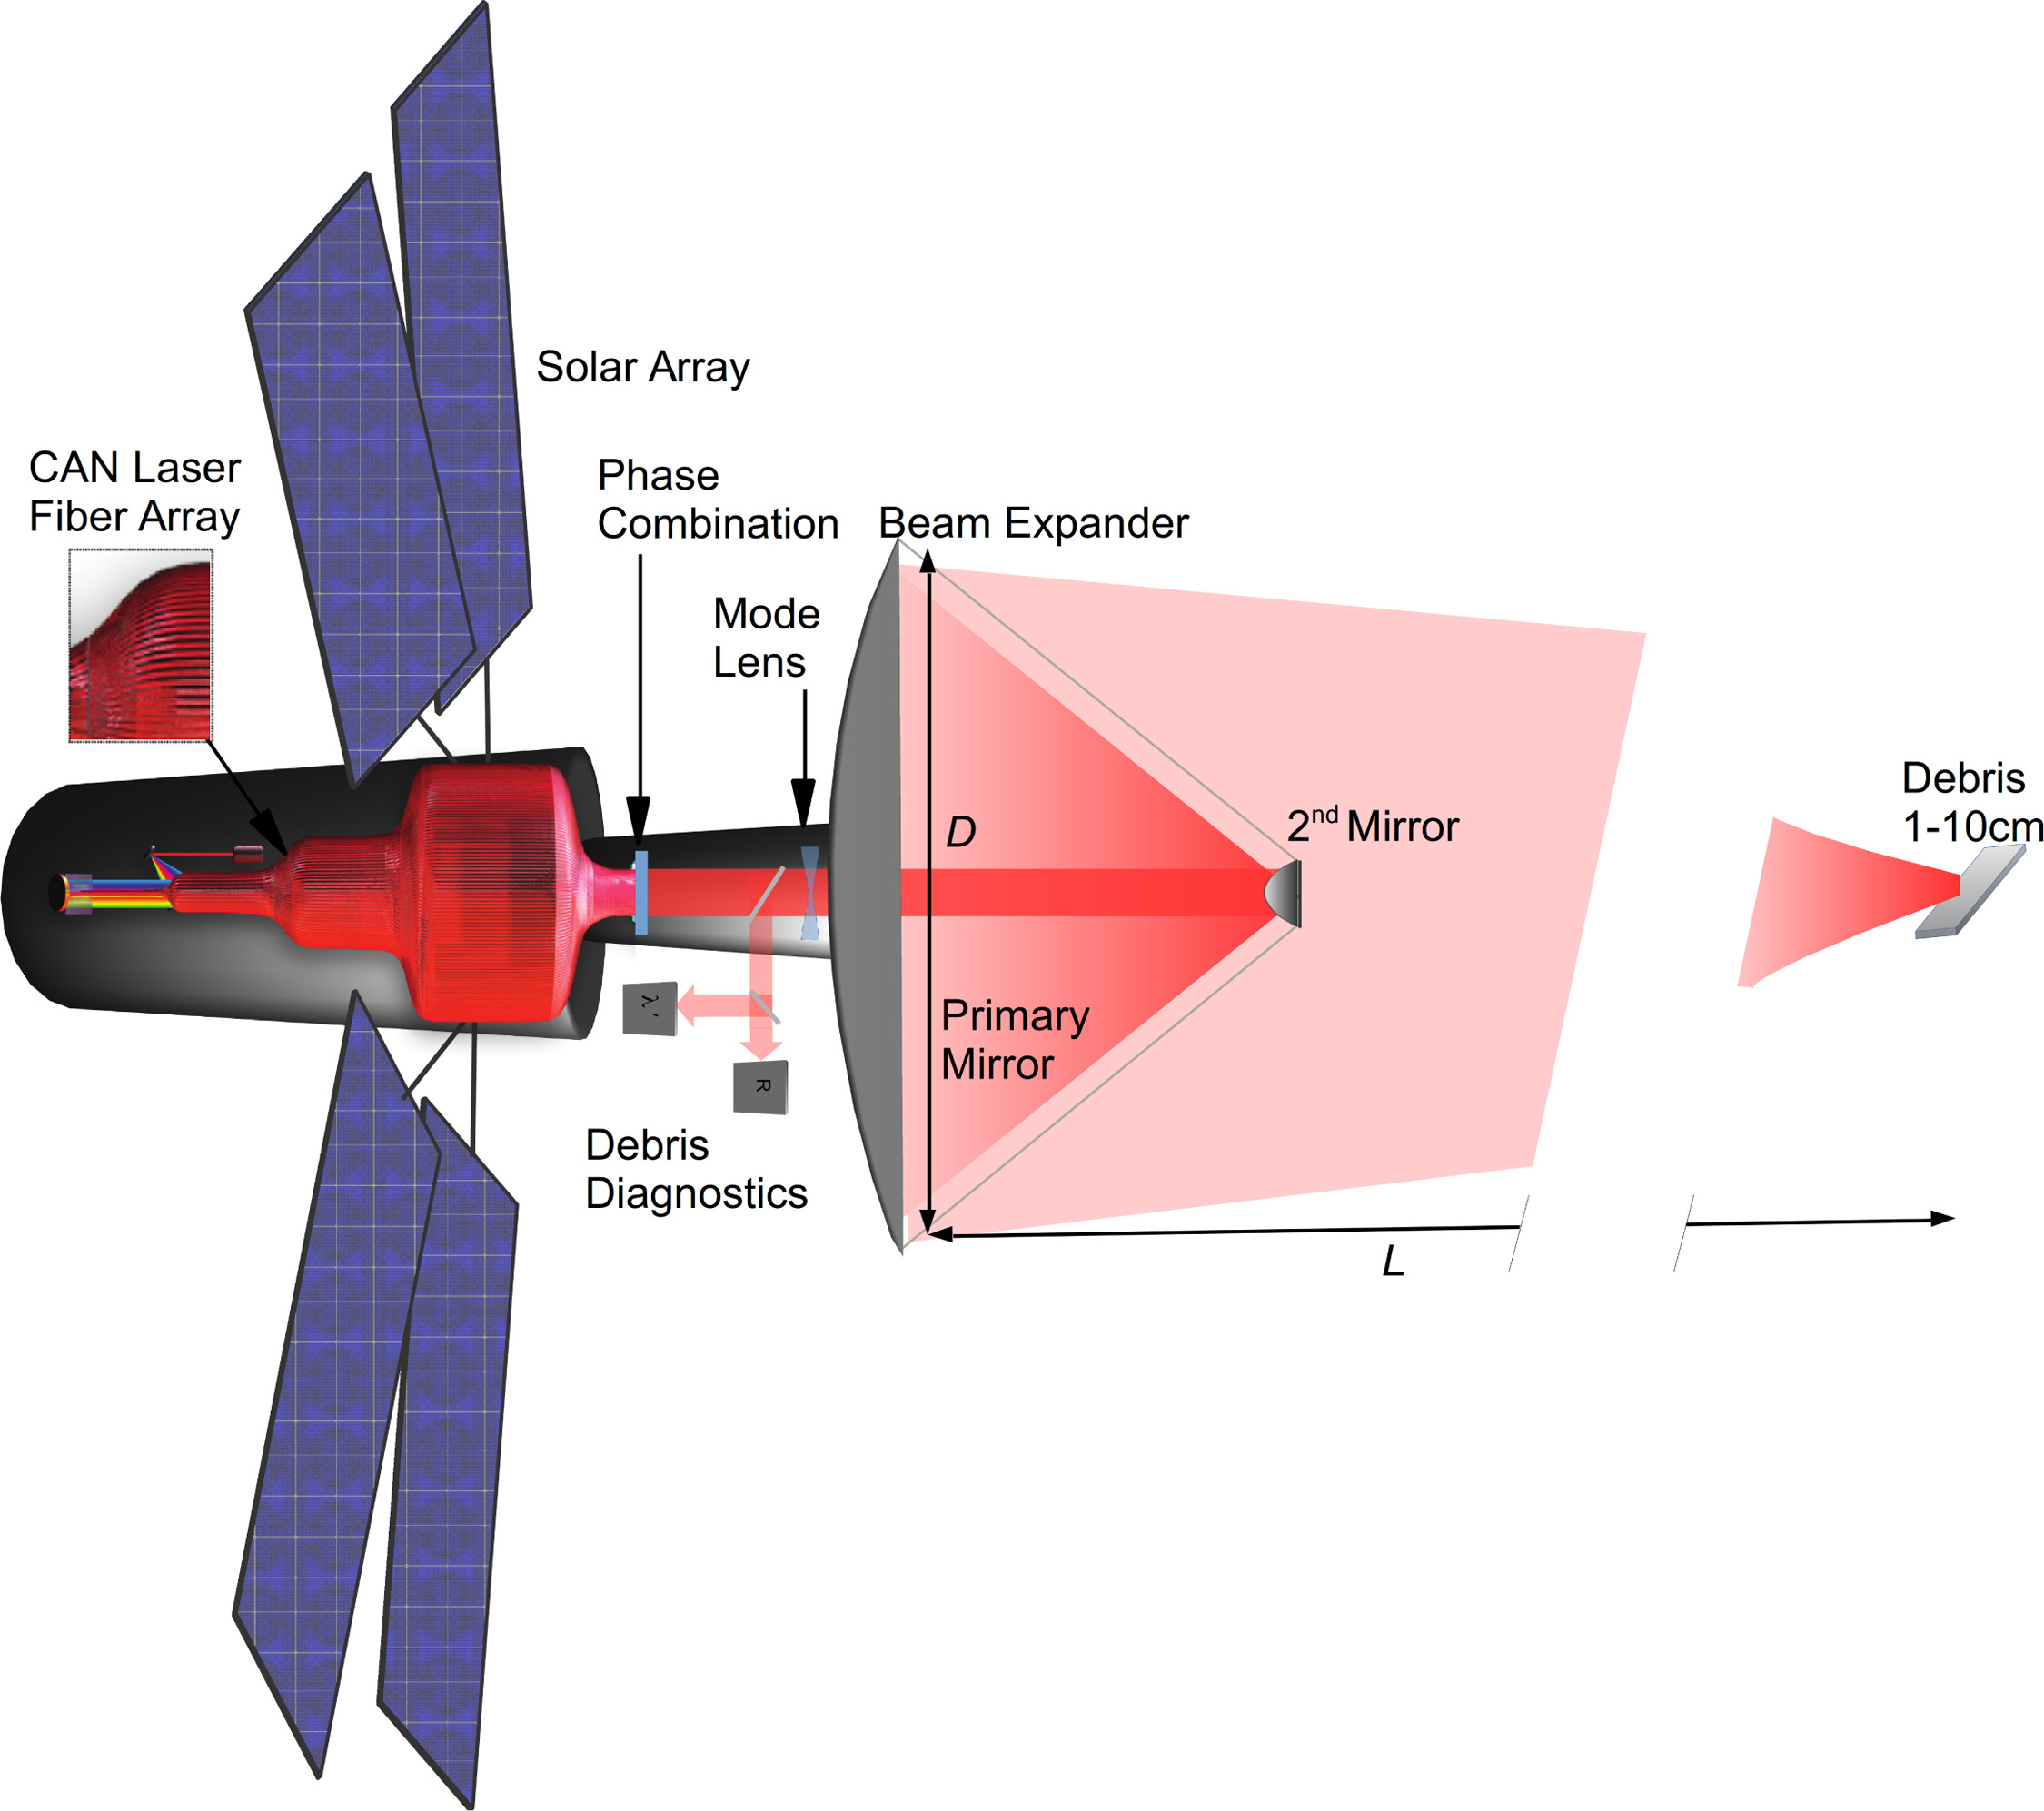
\includegraphics[width = 0.7\textwidth]{images/ICAN_Satellit.jpg}
	\caption{Aufbau des ICAN Sweepers nach \citet{soulard2014ican}}
	\label{icansat}
\end{figure}
\noindent
\autoref{icansat} zeigt einen beispielhaften Aufbau eines ICAN Sweepers. Neben dem bereits benannten ICAN Laser, welcher den Großteil des Satelliten einnimmt, werden zusätzlich noch Solarzellen zur Energieversorgung, sowie ein Teleskop und Module zur Debris Erfassung und Analyse, wie eine CCD-Kamera benötigt. Diese Kombination in einem System stellt besondere Anforderungen an den Satelliten, da neben einer möglichst kompakten und robusten Bauweise auch eine gute Wärmeableitung unabdingbar ist, um den Einsatz von Kühlmittel für den Laser möglichst zu vermeiden. 

\subsubsection{International Coherent Amplification Network Laser}
Der International Coherent Amplification Network Laser (ICAN) ist ein Lasersystem, welches 2014 vom International Coherent Amplification Network Consortium vorgestellt wurde. Das beim ICAN Laser für die Erzeugung des Lasers verwendete Glasfasernetzwerk kombiniert einen Petawatt Laser mit hoher Schussrate und zeichnet sich dabei durch eine hohe Energieeffizienz von circa \SI{30}{\percent} - \SI{50}{\percent} gegenüber herkömmlichen Petawatt Lasern sowie eine schnelle und genaue Anpassungsfähigkeit aus \citet{icanlaser}. Diese Eigenschaften erlauben die Integration in einem System wie dem ICAN Sweeper. Die hohe Energieeffizienz macht einen Betrieb unter einer solaren Energieversorgung mit hoher Schussrate erst möglich. Die Anpassungsfähigkeit erlaubt des Weiteren die Verwendung eines einzelnen Laser-Systems für Scanning, Tracking und den Beschuss etwaiger Objekte. Zusätzlich kann der Laser an die Oberflächeneigenschaften von Zielen angepasst werden, was eine weitere Effizienzsteigerung erlaubt. Die Energie, die pro Puls abgegeben werden kann, und somit auch die zu erreichende maximale Schuss-Reichweite des ICAN Sweepers sind maßgeblich von der Anzahl an verwendeten Glasfasern abhängig.
\begin{figure}[H]
	\centering
	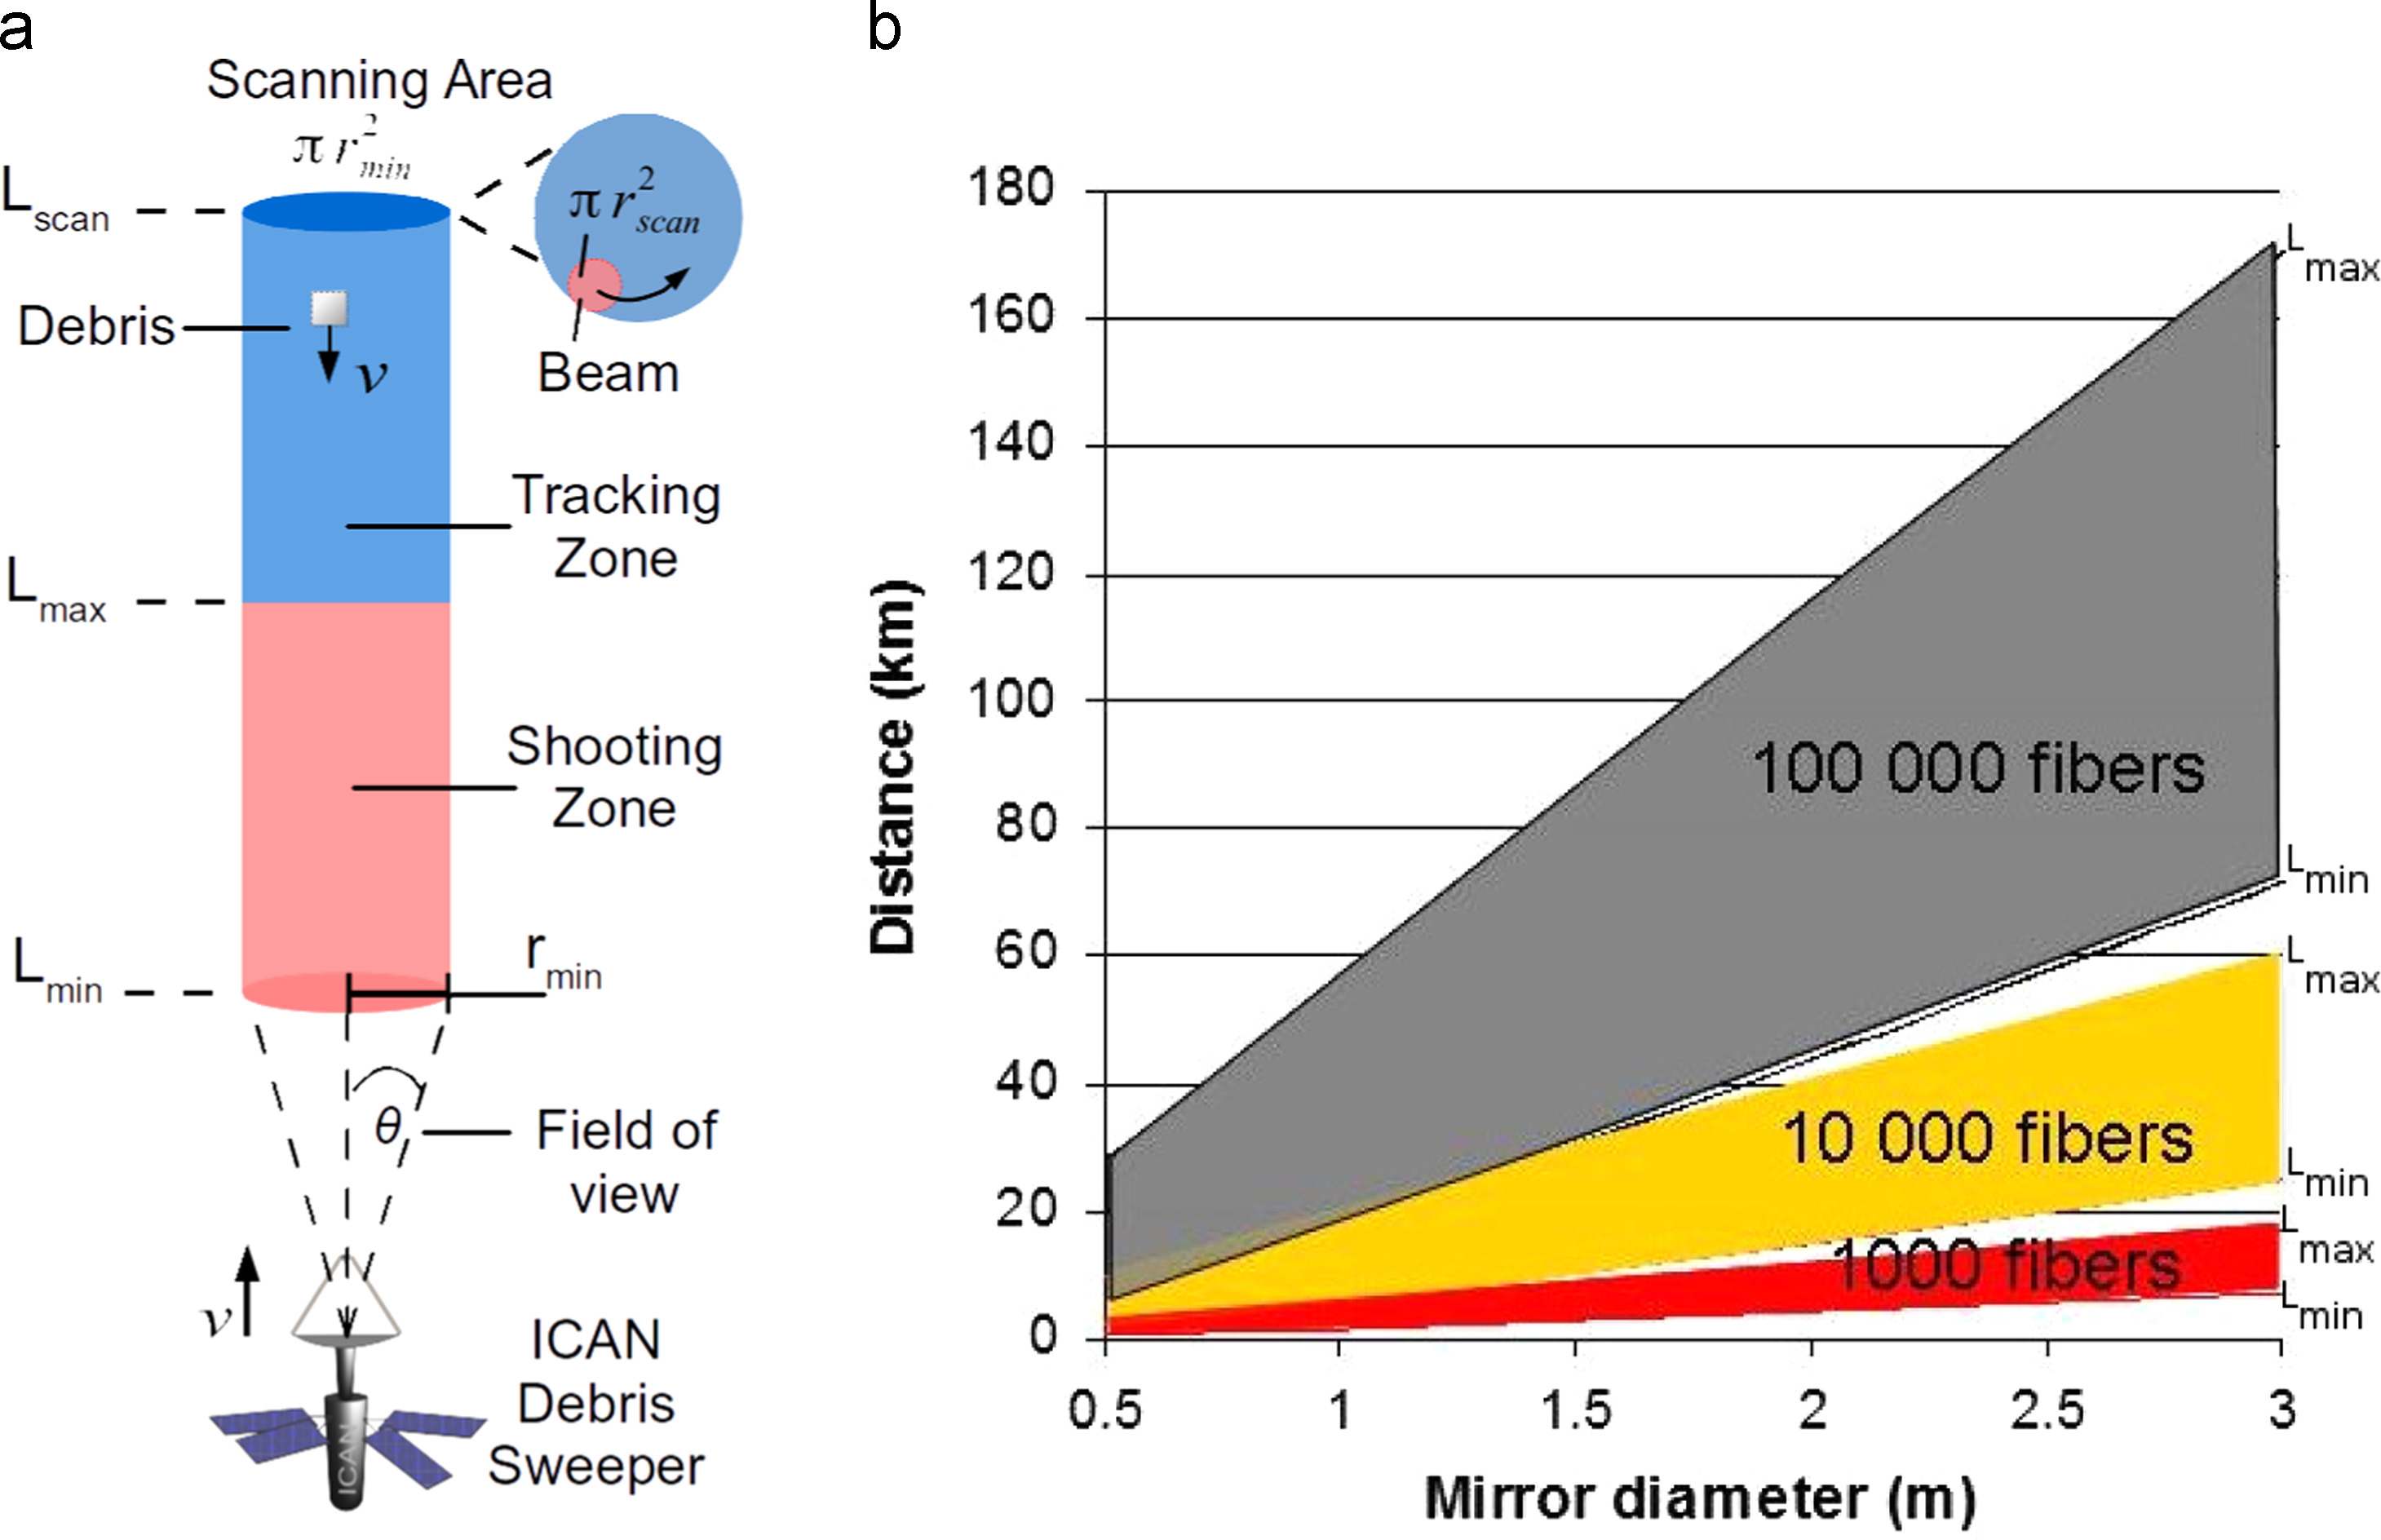
\includegraphics[width = 0.9\textwidth]{images/ICAN_reichwite.jpg}
	\caption{Reichweite des ICAN Sweepers in Abhängigkeit von der Glasfaseranzahl sowie des Durchmessers des primären Spiegels nach \citet{soulard2014ican}}
	\label{reichweite ICAN}
\end{figure}
\noindent
Wie anhand \autoref{reichweite ICAN} erkannt werden kann, können mit einem Spiegeldurchmesser von 3 Metern sowie 100000 Glasfasern Objekte in bis zu ~\SI{170}{\kilo\meter} Entfernung zum Absturz gebracht werden. Die Reichweite des Trackings liegt sogar noch darüber, da sie maßgeblich durch das kleinste detektierbare Signal limitiert wird. \citet{soulard2014ican} gibt hier Reichweiten von bis zu \SI{340}{\kilo\meter} bei 100000 Glasfasern an. Während ein Einsatz von möglichst vielen Glasfasern wünschenswert ist, so muss bei einem Erhöhen von deren Anzahl auch immer auf einen parallel steigenden Platzbedarf sowie ein erhöhtes Gewicht geachtet werden.

\subsubsection{Scanning, Tracking und Shooting}
Der ICAN Sweeper kann in drei Operationsmodi betrieben werden, dem Scanning-, Tracking- und Shooting-Mode. Ausschlaggebend für die Wahl des zu verwendenden Modus ist dabei die Entfernung zwischen dem Zielobjekt und dem Sweeper, wie \autoref{reichweite ICAN} zeigt. \\\\
Der Scanning Mode wird verwendet, solange sich kein Zielobjekt innerhalb der Tracking Zone befindet und ist in der Lage, neue Objekte zu detektieren. \\\\
Hierfür wird der Laser im Raum gestreut und durch eine Rotation des primären Spiegels im Raum verteilt. Potentielle Reflektionen von Objekten im Raum werden anschließend über eine CCD Kamera detektiert, die Relativbewegung kann des Weiteren über die empfangene Dopplerverschiebung bestimmt werden. Die Reichweite des Modus wird hauptsächlich von der Rotationsgeschwindigkeit des primären Spiegels bestimmt, da gewährleistet sein muss, dass der Laser jeden Bereich des vor dem Sweeper liegenden Raums abdeckt. Selbstverständlich muss die durch die Spiegelrotation maximal mögliche Reichweite auch durch die Glasfaseranzahl gewährleistet sein.\\\\
\noindent Sobald ein Objekt erfolgreich detektiert, die Flugbahn des ICAN Sweepers entsprechend angepasst wurde und sich das Objekt innerhalb der Tracking Zone befindet, kann mit der Analyse der Oberflächeneigenschaften begonnen werden. Hierbei werden unter anderem Reflektions- und Absorptionseigenschaften bestimmt und der Laser parallel entsprechend angepasst, um die Effizienz beim späteren Shooting zu erhöhen. Die benötigte Gesamtzeit für das Tracking variiert je nach Objektgröße und Glasfaseranzahl. Grundlegend kann jedoch gesagt werden, dass für größere Objekte und für eine erhöhte Glasfaseranzahl mehr Zeit benötigt wird, da die Anpassung des Lasers entsprechend länger dauert. In diesem Sinne gibt \citet{soulard2014ican} das Tracking für ein \SI{3}{\centi\meter} großes Objekt mit 1000 Glasfasern mit \SI{6}{\second} an, während mit 10000 Glasfasern bereits \SI{8}{\second} benötigt werden.\\\\
\noindent Sobald sich das Zielobjekt in der Shooting Zone befindet, kann mit der gezielten Verlangsamung unter zuhilfenahme der bereits beschriebenen Ablation begonnen werden. Die erwähnte Verlangsamung wird auch hier wieder durch einen wiederholten Beschuss durchgeführt, um sicherzustellen, dass das Objekt nicht zerstört wird. Die benötigte Gesamtenergie, um ein Objekt ausreichend zu verlangsamen, hängt dabei von der Flughöhe sowie der Objektgröße ab und beläuft sich nach \cite{soulard2014ican} auf circa \SI{e2}{\kilo\joule} - \SI{e3}{\kilo\joule} für \SI{3}{\centi\meter} - \SI{10}{\centi\meter} große Objekte in Flughöhen ab \SI{1000}{\kilo\meter}. Vor Erreichen der Shooting Zone wird eine Relativgeschwindigkeit von \SI{15}{\meter\per\second} zwischen Sweeper und Objekt angestrebt. Je nach benötigter Gesamtenergie muss dementsprechend die Schussrate variabel festgelegt werden.  Die minimale Reichweite für das Shooting $\mathrm{L_{min}}$ wird dabei durch die Teleskop-Brennweite des ICAN Sweepers bestimmt. 

\subsection{Fazit}
Die Entfernung von Weltraumschrott mit Hilfe von Laser-basierten Systemen bietet großes Potential, da sie gerade bei Objekten mit einer Größe zwischen \SI{1}{\centi\meter} und \SI{10}{\centi\meter} eine deutlich höhere Effizienz und Flexibilität aufweisen als mechanische Lösungen, wie sie bisher in diesem Bericht vorgestellt wurden. Bodengestützte Systeme, wie das LODR System, erlauben ein effizientes Entfernen von Objekten in variablen Größen, während eine gute Wartungsfähigkeit, konstante Energieversorgung und Treibstoffunabhängigkeit eine nahezu unbegrenzte Lebensdauer erlauben. Dies, sowie die Tatsache, dass keine Raketensysteme benötigt werden, um das System in eine Umlaufbahn zu bewegen, bedingen den großen Kostenvorteil im Vergleich zu Satellitengestützten Systemen. Zusätzlich hierzu können mehrere Objekte innerhalb eines Umlaufes zum Absturz gebracht werden, da keine wiederholte Orbitanpassung benötigt wird. Während all diese Vorteile stark für bodengestützte Systeme sprechen, besitzen diese mit dem Mangel an einer hochgenauen und effizienten Tracking- und Identifikations-Lösung jedoch auch einen entscheidenden Nachteil. Ohne eine ausreichend genaue Orbitbestimmung, stellt das Abschießen eines Objektes in \SI{1000}{\kilo\meter} Höhe mit einem Laser mit \SI{30}{\centi\meter} Durchmesser ein nahezu unlösbares Problem dar. Auch wenn mit dem Pusher Laser von \citet{p11q11orion} ein Lösungsansatz für diese Problematik existiert, so werden für dessen Umsetzung große Mengen Energie benötigt. Des Weiteren hängt die Größe der zu detektierenden Objekte stark von deren Albedo ab, wodurch das System nur noch beschränkt einsatzbereit ist. Zusätzlich zu dieser Problematik müssen außerdem auftretende atmosphärische Effekte berücksichtigt werden, die beim Durchdringen der Atmosphäre aufgrund der langen Laufzeit verstärkt auf den Laserstrahl einwirken.\\\\
\noindent Eine Lösung für diese Probleme stellt ein satellitenbasiertes System wie der ICAN Sweeper dar. Dieser ist, aufgrund seiner im Verlgeich niedrigen Distanz zu etwaigen Zielobjekten in der Lage, auch kleinere Objekte verlässlich mit hoher Genauigkeiten zu tracken und zu identifzieren. Der Solarbetrieb des Lasers verringert außerdem die benötigte Treibstoffmenge erheblich, was einen Betrieb des Systems über längere Zeit erlaubt. Dennoch ist ein solches Lasersystem aufgrund der fehlenden Wartungsmöglichkeiten stark in der Lebensdauer begrenzt. Des Weiteren entstehen hohe Kosten für die Platzierung des Satelliten im Orbit.\\\\
\noindent Während beide Implementierungen ihre Vor- und Nachteile besitzen, so würden sich diese doch zu großen Teilen ausgleichen, sollten sie kombiniert eingesetzt werden. So könnte beispielsweise ein satellitenbasiertes System wie der ICAN Sweeper eingesetzt werden, um Objekte zu tracken und zu katalogisieren. Diese Informationen könnten dann an ein bodengestütztes System weitergegeben werden, welches den Abschuss vornimmt.

\subsection{Aktuelle Umsetzungen}
Auch wenn die vorgestellten Verfahren technologisch umsetzbar wären, ist etwaiges bislang noch nicht erfolgt. Dies liegt zum einen daran, dass bislang noch kein ausreichendes gesellschaftliches Bewusstsein für die katastrophalen Folgen des steigenden Weltraumschrotts im All vorhanden ist und somit auch finanzielle Mittel für groß angelegte Missionen zur Schrottentfernung fehlen. Zum anderen besteht jedoch auch die Problematik einer unklaren Rechtslage bezüglich des Einsatzes eines Lasersystems entsprechender Größe und Stärke, dessen Anwendung in der Theorie auch auf aktive Satelliten in niedrigen Umlaufbahnen möglich ist. Auch wenn das Outer Space Treaty der UN von 1967 \citep{unost} eine grundlegende Regelung zu Waffensystemen im All vorgibt, wörtlich "The moon and other celestial bodies shall be used by all States Parties to the Treaty exclusively for peaceful purposes", so ist lediglich ein Einsatz und eine Platzierung von Massenvernichtungswaffen im All eindeutig untersagt, während normale Waffensysteme einer Interpretation des Begriffs "peaceful purposes" unterliegt. \citet{spacelaw} spricht hier von einer vorrangigen Interpretation des Begriffs im Rahmen einer nicht aggressiven Haltung, durch welche das All für militärische Fernerkundungs- und Spionagemissionen weiterhin offen ist. Auch wenn dies gewisse Rahmenbedingungen für einen Einsatz entsprechender Systeme schafft, so ist der Einsatz eines Lasersystems auch nach diesen zum jetzigen Zeitpunkt unklar, da ein solches zwar zu friedlichen Zwecken eingesetzt wird, unter bestimmten Gesetzgebungen jedoch auch als Waffe eingestuft werden kann. Diese Einstufung wird besonders relevant, sollte das 2008 von Russland vorgeschlagene "Proposed Prevention of an Arms Race in Space Treaty". \citet{unparos} verabschiedet werden, welches konkret die Platzierung eines jeden Objektes, welches eine Waffe trägt, sowie die Platzierung von Waffen jeder Art im All, vollständig untersagt. Auch wenn eine Verabschiedung eines solchen Treaties aufgrund einer Blockade der USA \citep{spacelaw} zur Zeit noch in weiter Ferne liegt, so ist dennoch klar, dass ein Einsatz von Lasersystemen zur Entfernung von Weltraumschrott nur mit Hilfe einer internationalen Regelung und regelmäßigen Kontrollen erfolgen sollte, um Spannungen in der Welt zu vermeiden. Dies könnte zum einen durch regelmäßige, gegenseitige Kontrollen einsetzender Länder erfolgen. Zum anderen wäre auch eine internationale Missionsleitung möglich, beispielsweise geleitet durch die UN.

\clearpage
\bibliography{bib/bib.bib}
\end{document}



